\RequirePackage{fix-cm}
\documentclass[ titlepage,numbers=noenddot,headinclude,
                footinclude=true,cleardoublepage=empty,abstractoff,
                BCOR=5mm,paper=letter,fontsize=12pt,
                american,
                openany
                ]{scrreprt}

% -*- root: thesis.tex -*-
% ****************************************************************************************************
% classicthesis-config.tex 
% formerly known as loadpackages.sty, classicthesis-ldpkg.sty, and classicthesis-preamble.sty 
% Use it at the beginning of your ClassicThesis.tex, or as a LaTeX Preamble 
% in your ClassicThesis.{tex,lyx} with % -*- root: thesis.tex -*-
% ****************************************************************************************************
% classicthesis-config.tex 
% formerly known as loadpackages.sty, classicthesis-ldpkg.sty, and classicthesis-preamble.sty 
% Use it at the beginning of your ClassicThesis.tex, or as a LaTeX Preamble 
% in your ClassicThesis.{tex,lyx} with % -*- root: thesis.tex -*-
% ****************************************************************************************************
% classicthesis-config.tex 
% formerly known as loadpackages.sty, classicthesis-ldpkg.sty, and classicthesis-preamble.sty 
% Use it at the beginning of your ClassicThesis.tex, or as a LaTeX Preamble 
% in your ClassicThesis.{tex,lyx} with \input{classicthesis-config}
% ****************************************************************************************************  
% If you like the classicthesis, then I would appreciate a postcard. 
% My address can be found in the file ClassicThesis.pdf. A collection 
% of the postcards I received so far is available online at 
% http://postcards.miede.de
% ****************************************************************************************************


% ****************************************************************************************************
% 0. Set the encoding of your files. UTF-8 is the only sensible encoding nowadays. If you can't read
% äöüßáéçèê∂åëæƒÏ€ then change the encoding setting in your editor, not the line below. If your editor
% does not support utf8 use another editor!
% ****************************************************************************************************
\PassOptionsToPackage{utf8}{inputenc}
	\usepackage{inputenc}

% ****************************************************************************************************
% 1. Configure classicthesis for your needs here, e.g., remove "drafting" below 
% in order to deactivate the time-stamp on the pages
% ****************************************************************************************************
% drafting
\PassOptionsToPackage{eulerchapternumbers,
listings,%
                    linedheaders,
					 pdfspacing,%floatperchapter,%linedheaders,%
					 subfig,beramono,eulermath,parts}{classicthesis}                                        
% ********************************************************************
% Available options for classicthesis.sty 
% (see ClassicThesis.pdf for more information):
% drafting
% parts nochapters linedheaders
% eulerchapternumbers beramono eulermath pdfspacing minionprospacing
% tocaligned dottedtoc manychapters
% listings floatperchapter subfig
% ********************************************************************


% ****************************************************************************************************
% 2. Personal data and user ad-hoc commands
% ****************************************************************************************************
\newcommand{\myTitle}{Meta Learning for Control\xspace}
\newcommand{\mySubtitle}{\xspace}
\newcommand{\myDegree}{\xspace}
\newcommand{\myName}{Yan Duan\xspace}
\newcommand{\myFaculty}{Pieter Abbeel\xspace}
\newcommand{\myDepartment}{Department of Electrical Engineering and Computer Sciences\xspace}
\newcommand{\myUni}{University of California, Berkeley\xspace}
\newcommand{\myLocation}{\xspace}
\newcommand{\myTime}{Fall, 2017\xspace}
% \newcommand{\myVersion}{version 4.2\xspace}

% ********************************************************************
% Setup, finetuning, and useful commands
% ********************************************************************
\newcounter{dummy} % necessary for correct hyperlinks (to index, bib, etc.)
\newlength{\abcd} % for ab..z string length calculation
\providecommand{\mLyX}{L\kern-.1667em\lower.25em\hbox{Y}\kern-.125emX\@}
\newcommand{\ie}{i.\,e.}
\newcommand{\Ie}{I.\,e.}
\newcommand{\eg}{e.\,g.}
\newcommand{\Eg}{E.\,g.} 
% ****************************************************************************************************


% ****************************************************************************************************
% 3. Loading some handy packages
% ****************************************************************************************************
% ******************************************************************** 
% Packages with options that might require adjustments
% ******************************************************************** 
%\PassOptionsToPackage{ngerman,american}{babel}   % change this to your language(s)
% Spanish languages need extra options in order to work with this template
%\PassOptionsToPackage{spanish,es-lcroman}{babel}
	\usepackage[american]{babel}                  

\usepackage{csquotes}
\PassOptionsToPackage{%
    backend=biber, %instead of bibtex
	%%backend=bibtex8,
    bibencoding=ascii,%
	language=american,%auto,%
    uniquename=full,
    uniquelist=false,
	%%style=numeric-comp,%
    %% style=authoryear-comp, % Author 1999, 2010
    bibstyle=authoryear,
    dashed=false, % dashed: substitute rep. author with ---
    style=authoryear,%alphabetic,
    citestyle=authoryear,%alphabetic,
    sorting=nyt, % name, year, title
    maxnames=2,
    minnames=1,
    maxcitenames=2,
    mincitenames=1,
    maxbibnames=100,%2, % default: 3, et al.
    minbibnames=100, % default: 3, et al.
    backref=true,
    giveninits=false,
    natbib=true % natbib compatibility mode (\citep and \citet still work)
}{biblatex}
    \usepackage{biblatex}
%\renewcommand*{\bibfont}{\small}
\DeclareLanguageMapping{american}{american-apa}
\usepackage{xpatch}

\xpatchbibmacro{textcite}{%
          {\usebibmacro{cite:label}%
       \setunit{%
         \global\booltrue{cbx:parens}%
         \addspace\bibopenparen}%
       \ifnumequal{\value{citecount}}{1}
         {\usebibmacro{prenote}}
         {}%
       \ifthenelse{\ifciteibid\AND\NOT\iffirstonpage}
         {\usebibmacro{cite:ibid}}
         {\usebibmacro{cite:labelyear+extrayear}}}
}{%
          {\usebibmacro{cite:label}%
       \setunit{%
         \global\booltrue{cbx:parens}%
         \addspace\bibopenparen}%
       \ifnumequal{\value{citecount}}{1}
         {\usebibmacro{prenote}}
         {}%
      \usebibmacro{cite:labelyear+extrayear}}
}{}{}

\xpatchbibmacro{textcite}{%
             {\ifthenelse{\ifciteibid\AND\NOT\iffirstonpage}
        {\usebibmacro{cite:ibid}}
        {\usebibmacro{cite:labelyear+extrayear}}}%
}{%
             {\usebibmacro{cite:labelyear+extrayear}}%
}{}{}

% \PassOptionsToPackage{fleqn}{amsmath}       % math environments and more by the AMS 
    \usepackage{amsmath}
% \setlength{\mathindent}{0cm}
% ******************************************************************** 
% General useful packages
% ******************************************************************** 
\PassOptionsToPackage{T1}{fontenc} % T2A for cyrillics
    \usepackage{fontenc}     
\usepackage{textcomp} % fix warning with missing font shapes
\usepackage{scrhack} % fix warnings when using KOMA with listings package          
\usepackage{xspace} % to get the spacing after macros right  
\usepackage{mparhack} % get marginpar right
%\usepackage[latest]{latexrelease} % will be used once available in more distributions (ISSUE #107)
\PassOptionsToPackage{printonlyused,smaller}{acronym} 
    \usepackage{acronym} % nice macros for handling all acronyms in the thesis
    %\renewcommand{\bflabel}[1]{{#1}\hfill} % fix the list of acronyms --> no longer working
    %\renewcommand*{\acsfont}[1]{\textsc{#1}} 
    \renewcommand*{\aclabelfont}[1]{\acsfont{#1}}
% ****************************************************************************************************


% ****************************************************************************************************
% 4. Setup floats: tables, (sub)figures, and captions
% ****************************************************************************************************
\usepackage{tabularx} % better tables
    \setlength{\extrarowheight}{3pt} % increase table row height
\newcommand{\tableheadline}[1]{\multicolumn{1}{c}{\spacedlowsmallcaps{#1}}}
\newcommand{\myfloatalign}{\centering} % to be used with each float for alignment
\usepackage{caption}
% Thanks to cgnieder and Claus Lahiri
% http://tex.stackexchange.com/questions/69349/spacedlowsmallcaps-in-caption-label
% [REMOVED DUE TO OTHER PROBLEMS, SEE ISSUE #82]    
%\DeclareCaptionLabelFormat{smallcaps}{\bothIfFirst{#1}{~}\MakeTextLowercase{\textsc{#2}}}
%\captionsetup{font=small,labelformat=smallcaps} % format=hang,
\captionsetup{font=small} % format=hang,
%\usepackage{subfig}  
% ****************************************************************************************************


% ****************************************************************************************************
% 5. Setup code listings
% ****************************************************************************************************
\usepackage{listings} 
%\lstset{emph={trueIndex,root},emphstyle=\color{BlueViolet}}%\underbar} % for special keywords
\lstset{language=[LaTeX]Tex,%C++,
    morekeywords={PassOptionsToPackage,selectlanguage},
    keywordstyle=\color{RoyalBlue},%\bfseries,
    basicstyle=\small\ttfamily,
    %identifierstyle=\color{NavyBlue},
    commentstyle=\color{Green}\ttfamily,
    stringstyle=\rmfamily,
    numbers=none,%left,%
    numberstyle=\scriptsize,%\tiny
    stepnumber=5,
    numbersep=8pt,
    showstringspaces=false,
    breaklines=true,
    %frameround=ftff,
    %frame=single,
    belowcaptionskip=.75\baselineskip
    %frame=L
} 
% ****************************************************************************************************             


% ****************************************************************************************************
% 6. PDFLaTeX, hyperreferences and citation backreferences
% ****************************************************************************************************
% ********************************************************************
% Using PDFLaTeX
% ********************************************************************
\PassOptionsToPackage{pdftex,hyperfootnotes=false,pdfpagelabels}{hyperref}
    \usepackage{hyperref}  % backref linktocpage pagebackref
\pdfcompresslevel=9
\pdfadjustspacing=1 
\PassOptionsToPackage{pdftex}{graphicx}
    \usepackage{graphicx} 
 

% ********************************************************************
% Hyperreferences
% ********************************************************************
\hypersetup{%
    %draft, % = no hyperlinking at all (useful in b/w printouts)
    colorlinks=true, linktocpage=true, pdfstartpage=3, pdfstartview=FitV,%
    % uncomment the following line if you want to have black links (e.g., for printing)
    %colorlinks=false, linktocpage=false, pdfstartpage=3, pdfstartview=FitV, pdfborder={0 0 0},%
    breaklinks=true, pdfpagemode=UseNone, pageanchor=true, pdfpagemode=UseOutlines,%
    plainpages=false, bookmarksnumbered, bookmarksopen=true, bookmarksopenlevel=1,%
    hypertexnames=true, pdfhighlight=/O,%nesting=true,%frenchlinks,%
    urlcolor=webbrown, linkcolor=RoyalBlue, citecolor=berkeleyblue, %pagecolor=RoyalBlue,%
    %urlcolor=Black, linkcolor=Black, citecolor=Black, %pagecolor=Black,%
    pdftitle={\myTitle},%
    pdfauthor={\textcopyright\ \myName, \myUni, \myFaculty},%
    pdfsubject={},%
    pdfkeywords={},%
    pdfcreator={pdfLaTeX},%
    pdfproducer={LaTeX with hyperref and classicthesis}%
}   

% ********************************************************************
% Setup autoreferences
% ********************************************************************
% There are some issues regarding autorefnames
% http://www.ureader.de/msg/136221647.aspx
% http://www.tex.ac.uk/cgi-bin/texfaq2html?label=latexwords
% you have to redefine the makros for the 
% language you use, e.g., american, ngerman
% (as chosen when loading babel/AtBeginDocument)
% ********************************************************************
\makeatletter
%\usepackage[english]{babel}

\@ifpackageloaded{babel}%
    {%
       \addto\extrasamerican{%
			\renewcommand*{\figureautorefname}{Figure}%
			\renewcommand*{\tableautorefname}{Table}%
			\renewcommand*{\partautorefname}{Part}%
			\renewcommand*{\chapterautorefname}{Chapter}%
			\renewcommand*{\sectionautorefname}{Section}%
			\renewcommand*{\subsectionautorefname}{Section}%
			\renewcommand*{\subsubsectionautorefname}{Section}%     
                }%
       \addto\extrasngerman{% 
			\renewcommand*{\paragraphautorefname}{Absatz}%
			\renewcommand*{\subparagraphautorefname}{Unterabsatz}%
			\renewcommand*{\footnoteautorefname}{Fu\"snote}%
			\renewcommand*{\FancyVerbLineautorefname}{Zeile}%
			\renewcommand*{\theoremautorefname}{Theorem}%
			\renewcommand*{\appendixautorefname}{Anhang}%
			\renewcommand*{\equationautorefname}{Gleichung}%        
			\renewcommand*{\itemautorefname}{Punkt}%
                }%  
            % Fix to getting autorefs for subfigures right (thanks to Belinda Vogt for changing the definition)
            \providecommand{\subfigureautorefname}{\figureautorefname}%             
    }{\relax}
\makeatother


% ****************************************************************************************************
% 7. Last calls before the bar closes
% ****************************************************************************************************
% ********************************************************************
% Development Stuff
% ********************************************************************
\listfiles
%\PassOptionsToPackage{l2tabu,orthodox,abort}{nag}
%   \usepackage{nag}
%\PassOptionsToPackage{warning, all}{onlyamsmath}
%   \usepackage{onlyamsmath}

% ********************************************************************
% Last, but not least...
% ********************************************************************
\usepackage{classicthesis} 
% ****************************************************************************************************


% ****************************************************************************************************
% 8. Further adjustments (experimental)
% ****************************************************************************************************
% ********************************************************************
% Changing the text area
% ********************************************************************
%\linespread{1.05} % a bit more for Palatino
%\areaset[current]{312pt}{761pt} % 686 (factor 2.2) + 33 head + 42 head \the\footskip
%\setlength{\marginparwidth}{7em}%
%\setlength{\marginparsep}{2em}%

% ********************************************************************
% Using different fonts
% ********************************************************************
%\usepackage[oldstylenums]{kpfonts} % oldstyle notextcomp
%\usepackage[osf]{libertine}
%\usepackage[light,condensed,math]{iwona}
%\renewcommand{\sfdefault}{iwona}
%\usepackage{lmodern} % <-- no osf support :-(
%\usepackage{cfr-lm} % 
%\usepackage[urw-garamond]{mathdesign} <-- no osf support :-(
%\usepackage[default,osfigures]{opensans} % scale=0.95 
%\usepackage[sfdefault]{FiraSans}
% ****************************************************************************************************

% ****************************************************************************************************  
% If you like the classicthesis, then I would appreciate a postcard. 
% My address can be found in the file ClassicThesis.pdf. A collection 
% of the postcards I received so far is available online at 
% http://postcards.miede.de
% ****************************************************************************************************


% ****************************************************************************************************
% 0. Set the encoding of your files. UTF-8 is the only sensible encoding nowadays. If you can't read
% äöüßáéçèê∂åëæƒÏ€ then change the encoding setting in your editor, not the line below. If your editor
% does not support utf8 use another editor!
% ****************************************************************************************************
\PassOptionsToPackage{utf8}{inputenc}
	\usepackage{inputenc}

% ****************************************************************************************************
% 1. Configure classicthesis for your needs here, e.g., remove "drafting" below 
% in order to deactivate the time-stamp on the pages
% ****************************************************************************************************
% drafting
\PassOptionsToPackage{eulerchapternumbers,
listings,%
                    linedheaders,
					 pdfspacing,%floatperchapter,%linedheaders,%
					 subfig,beramono,eulermath,parts}{classicthesis}                                        
% ********************************************************************
% Available options for classicthesis.sty 
% (see ClassicThesis.pdf for more information):
% drafting
% parts nochapters linedheaders
% eulerchapternumbers beramono eulermath pdfspacing minionprospacing
% tocaligned dottedtoc manychapters
% listings floatperchapter subfig
% ********************************************************************


% ****************************************************************************************************
% 2. Personal data and user ad-hoc commands
% ****************************************************************************************************
\newcommand{\myTitle}{Meta Learning for Control\xspace}
\newcommand{\mySubtitle}{\xspace}
\newcommand{\myDegree}{\xspace}
\newcommand{\myName}{Yan Duan\xspace}
\newcommand{\myFaculty}{Pieter Abbeel\xspace}
\newcommand{\myDepartment}{Department of Electrical Engineering and Computer Sciences\xspace}
\newcommand{\myUni}{University of California, Berkeley\xspace}
\newcommand{\myLocation}{\xspace}
\newcommand{\myTime}{Fall, 2017\xspace}
% \newcommand{\myVersion}{version 4.2\xspace}

% ********************************************************************
% Setup, finetuning, and useful commands
% ********************************************************************
\newcounter{dummy} % necessary for correct hyperlinks (to index, bib, etc.)
\newlength{\abcd} % for ab..z string length calculation
\providecommand{\mLyX}{L\kern-.1667em\lower.25em\hbox{Y}\kern-.125emX\@}
\newcommand{\ie}{i.\,e.}
\newcommand{\Ie}{I.\,e.}
\newcommand{\eg}{e.\,g.}
\newcommand{\Eg}{E.\,g.} 
% ****************************************************************************************************


% ****************************************************************************************************
% 3. Loading some handy packages
% ****************************************************************************************************
% ******************************************************************** 
% Packages with options that might require adjustments
% ******************************************************************** 
%\PassOptionsToPackage{ngerman,american}{babel}   % change this to your language(s)
% Spanish languages need extra options in order to work with this template
%\PassOptionsToPackage{spanish,es-lcroman}{babel}
	\usepackage[american]{babel}                  

\usepackage{csquotes}
\PassOptionsToPackage{%
    backend=biber, %instead of bibtex
	%%backend=bibtex8,
    bibencoding=ascii,%
	language=american,%auto,%
    uniquename=full,
    uniquelist=false,
	%%style=numeric-comp,%
    %% style=authoryear-comp, % Author 1999, 2010
    bibstyle=authoryear,
    dashed=false, % dashed: substitute rep. author with ---
    style=authoryear,%alphabetic,
    citestyle=authoryear,%alphabetic,
    sorting=nyt, % name, year, title
    maxnames=2,
    minnames=1,
    maxcitenames=2,
    mincitenames=1,
    maxbibnames=100,%2, % default: 3, et al.
    minbibnames=100, % default: 3, et al.
    backref=true,
    giveninits=false,
    natbib=true % natbib compatibility mode (\citep and \citet still work)
}{biblatex}
    \usepackage{biblatex}
%\renewcommand*{\bibfont}{\small}
\DeclareLanguageMapping{american}{american-apa}
\usepackage{xpatch}

\xpatchbibmacro{textcite}{%
          {\usebibmacro{cite:label}%
       \setunit{%
         \global\booltrue{cbx:parens}%
         \addspace\bibopenparen}%
       \ifnumequal{\value{citecount}}{1}
         {\usebibmacro{prenote}}
         {}%
       \ifthenelse{\ifciteibid\AND\NOT\iffirstonpage}
         {\usebibmacro{cite:ibid}}
         {\usebibmacro{cite:labelyear+extrayear}}}
}{%
          {\usebibmacro{cite:label}%
       \setunit{%
         \global\booltrue{cbx:parens}%
         \addspace\bibopenparen}%
       \ifnumequal{\value{citecount}}{1}
         {\usebibmacro{prenote}}
         {}%
      \usebibmacro{cite:labelyear+extrayear}}
}{}{}

\xpatchbibmacro{textcite}{%
             {\ifthenelse{\ifciteibid\AND\NOT\iffirstonpage}
        {\usebibmacro{cite:ibid}}
        {\usebibmacro{cite:labelyear+extrayear}}}%
}{%
             {\usebibmacro{cite:labelyear+extrayear}}%
}{}{}

% \PassOptionsToPackage{fleqn}{amsmath}       % math environments and more by the AMS 
    \usepackage{amsmath}
% \setlength{\mathindent}{0cm}
% ******************************************************************** 
% General useful packages
% ******************************************************************** 
\PassOptionsToPackage{T1}{fontenc} % T2A for cyrillics
    \usepackage{fontenc}     
\usepackage{textcomp} % fix warning with missing font shapes
\usepackage{scrhack} % fix warnings when using KOMA with listings package          
\usepackage{xspace} % to get the spacing after macros right  
\usepackage{mparhack} % get marginpar right
%\usepackage[latest]{latexrelease} % will be used once available in more distributions (ISSUE #107)
\PassOptionsToPackage{printonlyused,smaller}{acronym} 
    \usepackage{acronym} % nice macros for handling all acronyms in the thesis
    %\renewcommand{\bflabel}[1]{{#1}\hfill} % fix the list of acronyms --> no longer working
    %\renewcommand*{\acsfont}[1]{\textsc{#1}} 
    \renewcommand*{\aclabelfont}[1]{\acsfont{#1}}
% ****************************************************************************************************


% ****************************************************************************************************
% 4. Setup floats: tables, (sub)figures, and captions
% ****************************************************************************************************
\usepackage{tabularx} % better tables
    \setlength{\extrarowheight}{3pt} % increase table row height
\newcommand{\tableheadline}[1]{\multicolumn{1}{c}{\spacedlowsmallcaps{#1}}}
\newcommand{\myfloatalign}{\centering} % to be used with each float for alignment
\usepackage{caption}
% Thanks to cgnieder and Claus Lahiri
% http://tex.stackexchange.com/questions/69349/spacedlowsmallcaps-in-caption-label
% [REMOVED DUE TO OTHER PROBLEMS, SEE ISSUE #82]    
%\DeclareCaptionLabelFormat{smallcaps}{\bothIfFirst{#1}{~}\MakeTextLowercase{\textsc{#2}}}
%\captionsetup{font=small,labelformat=smallcaps} % format=hang,
\captionsetup{font=small} % format=hang,
%\usepackage{subfig}  
% ****************************************************************************************************


% ****************************************************************************************************
% 5. Setup code listings
% ****************************************************************************************************
\usepackage{listings} 
%\lstset{emph={trueIndex,root},emphstyle=\color{BlueViolet}}%\underbar} % for special keywords
\lstset{language=[LaTeX]Tex,%C++,
    morekeywords={PassOptionsToPackage,selectlanguage},
    keywordstyle=\color{RoyalBlue},%\bfseries,
    basicstyle=\small\ttfamily,
    %identifierstyle=\color{NavyBlue},
    commentstyle=\color{Green}\ttfamily,
    stringstyle=\rmfamily,
    numbers=none,%left,%
    numberstyle=\scriptsize,%\tiny
    stepnumber=5,
    numbersep=8pt,
    showstringspaces=false,
    breaklines=true,
    %frameround=ftff,
    %frame=single,
    belowcaptionskip=.75\baselineskip
    %frame=L
} 
% ****************************************************************************************************             


% ****************************************************************************************************
% 6. PDFLaTeX, hyperreferences and citation backreferences
% ****************************************************************************************************
% ********************************************************************
% Using PDFLaTeX
% ********************************************************************
\PassOptionsToPackage{pdftex,hyperfootnotes=false,pdfpagelabels}{hyperref}
    \usepackage{hyperref}  % backref linktocpage pagebackref
\pdfcompresslevel=9
\pdfadjustspacing=1 
\PassOptionsToPackage{pdftex}{graphicx}
    \usepackage{graphicx} 
 

% ********************************************************************
% Hyperreferences
% ********************************************************************
\hypersetup{%
    %draft, % = no hyperlinking at all (useful in b/w printouts)
    colorlinks=true, linktocpage=true, pdfstartpage=3, pdfstartview=FitV,%
    % uncomment the following line if you want to have black links (e.g., for printing)
    %colorlinks=false, linktocpage=false, pdfstartpage=3, pdfstartview=FitV, pdfborder={0 0 0},%
    breaklinks=true, pdfpagemode=UseNone, pageanchor=true, pdfpagemode=UseOutlines,%
    plainpages=false, bookmarksnumbered, bookmarksopen=true, bookmarksopenlevel=1,%
    hypertexnames=true, pdfhighlight=/O,%nesting=true,%frenchlinks,%
    urlcolor=webbrown, linkcolor=RoyalBlue, citecolor=berkeleyblue, %pagecolor=RoyalBlue,%
    %urlcolor=Black, linkcolor=Black, citecolor=Black, %pagecolor=Black,%
    pdftitle={\myTitle},%
    pdfauthor={\textcopyright\ \myName, \myUni, \myFaculty},%
    pdfsubject={},%
    pdfkeywords={},%
    pdfcreator={pdfLaTeX},%
    pdfproducer={LaTeX with hyperref and classicthesis}%
}   

% ********************************************************************
% Setup autoreferences
% ********************************************************************
% There are some issues regarding autorefnames
% http://www.ureader.de/msg/136221647.aspx
% http://www.tex.ac.uk/cgi-bin/texfaq2html?label=latexwords
% you have to redefine the makros for the 
% language you use, e.g., american, ngerman
% (as chosen when loading babel/AtBeginDocument)
% ********************************************************************
\makeatletter
%\usepackage[english]{babel}

\@ifpackageloaded{babel}%
    {%
       \addto\extrasamerican{%
			\renewcommand*{\figureautorefname}{Figure}%
			\renewcommand*{\tableautorefname}{Table}%
			\renewcommand*{\partautorefname}{Part}%
			\renewcommand*{\chapterautorefname}{Chapter}%
			\renewcommand*{\sectionautorefname}{Section}%
			\renewcommand*{\subsectionautorefname}{Section}%
			\renewcommand*{\subsubsectionautorefname}{Section}%     
                }%
       \addto\extrasngerman{% 
			\renewcommand*{\paragraphautorefname}{Absatz}%
			\renewcommand*{\subparagraphautorefname}{Unterabsatz}%
			\renewcommand*{\footnoteautorefname}{Fu\"snote}%
			\renewcommand*{\FancyVerbLineautorefname}{Zeile}%
			\renewcommand*{\theoremautorefname}{Theorem}%
			\renewcommand*{\appendixautorefname}{Anhang}%
			\renewcommand*{\equationautorefname}{Gleichung}%        
			\renewcommand*{\itemautorefname}{Punkt}%
                }%  
            % Fix to getting autorefs for subfigures right (thanks to Belinda Vogt for changing the definition)
            \providecommand{\subfigureautorefname}{\figureautorefname}%             
    }{\relax}
\makeatother


% ****************************************************************************************************
% 7. Last calls before the bar closes
% ****************************************************************************************************
% ********************************************************************
% Development Stuff
% ********************************************************************
\listfiles
%\PassOptionsToPackage{l2tabu,orthodox,abort}{nag}
%   \usepackage{nag}
%\PassOptionsToPackage{warning, all}{onlyamsmath}
%   \usepackage{onlyamsmath}

% ********************************************************************
% Last, but not least...
% ********************************************************************
\usepackage{classicthesis} 
% ****************************************************************************************************


% ****************************************************************************************************
% 8. Further adjustments (experimental)
% ****************************************************************************************************
% ********************************************************************
% Changing the text area
% ********************************************************************
%\linespread{1.05} % a bit more for Palatino
%\areaset[current]{312pt}{761pt} % 686 (factor 2.2) + 33 head + 42 head \the\footskip
%\setlength{\marginparwidth}{7em}%
%\setlength{\marginparsep}{2em}%

% ********************************************************************
% Using different fonts
% ********************************************************************
%\usepackage[oldstylenums]{kpfonts} % oldstyle notextcomp
%\usepackage[osf]{libertine}
%\usepackage[light,condensed,math]{iwona}
%\renewcommand{\sfdefault}{iwona}
%\usepackage{lmodern} % <-- no osf support :-(
%\usepackage{cfr-lm} % 
%\usepackage[urw-garamond]{mathdesign} <-- no osf support :-(
%\usepackage[default,osfigures]{opensans} % scale=0.95 
%\usepackage[sfdefault]{FiraSans}
% ****************************************************************************************************

% ****************************************************************************************************  
% If you like the classicthesis, then I would appreciate a postcard. 
% My address can be found in the file ClassicThesis.pdf. A collection 
% of the postcards I received so far is available online at 
% http://postcards.miede.de
% ****************************************************************************************************


% ****************************************************************************************************
% 0. Set the encoding of your files. UTF-8 is the only sensible encoding nowadays. If you can't read
% äöüßáéçèê∂åëæƒÏ€ then change the encoding setting in your editor, not the line below. If your editor
% does not support utf8 use another editor!
% ****************************************************************************************************
\PassOptionsToPackage{utf8}{inputenc}
	\usepackage{inputenc}

% ****************************************************************************************************
% 1. Configure classicthesis for your needs here, e.g., remove "drafting" below 
% in order to deactivate the time-stamp on the pages
% ****************************************************************************************************
% drafting
\PassOptionsToPackage{eulerchapternumbers,
listings,%
                    linedheaders,
					 pdfspacing,%floatperchapter,%linedheaders,%
					 subfig,beramono,eulermath,parts}{classicthesis}                                        
% ********************************************************************
% Available options for classicthesis.sty 
% (see ClassicThesis.pdf for more information):
% drafting
% parts nochapters linedheaders
% eulerchapternumbers beramono eulermath pdfspacing minionprospacing
% tocaligned dottedtoc manychapters
% listings floatperchapter subfig
% ********************************************************************


% ****************************************************************************************************
% 2. Personal data and user ad-hoc commands
% ****************************************************************************************************
\newcommand{\myTitle}{Meta Learning for Control\xspace}
\newcommand{\mySubtitle}{\xspace}
\newcommand{\myDegree}{\xspace}
\newcommand{\myName}{Yan Duan\xspace}
\newcommand{\myFaculty}{Pieter Abbeel\xspace}
\newcommand{\myDepartment}{Department of Electrical Engineering and Computer Sciences\xspace}
\newcommand{\myUni}{University of California, Berkeley\xspace}
\newcommand{\myLocation}{\xspace}
\newcommand{\myTime}{Fall, 2017\xspace}
% \newcommand{\myVersion}{version 4.2\xspace}

% ********************************************************************
% Setup, finetuning, and useful commands
% ********************************************************************
\newcounter{dummy} % necessary for correct hyperlinks (to index, bib, etc.)
\newlength{\abcd} % for ab..z string length calculation
\providecommand{\mLyX}{L\kern-.1667em\lower.25em\hbox{Y}\kern-.125emX\@}
\newcommand{\ie}{i.\,e.}
\newcommand{\Ie}{I.\,e.}
\newcommand{\eg}{e.\,g.}
\newcommand{\Eg}{E.\,g.} 
% ****************************************************************************************************


% ****************************************************************************************************
% 3. Loading some handy packages
% ****************************************************************************************************
% ******************************************************************** 
% Packages with options that might require adjustments
% ******************************************************************** 
%\PassOptionsToPackage{ngerman,american}{babel}   % change this to your language(s)
% Spanish languages need extra options in order to work with this template
%\PassOptionsToPackage{spanish,es-lcroman}{babel}
	\usepackage[american]{babel}                  

\usepackage{csquotes}
\PassOptionsToPackage{%
    backend=biber, %instead of bibtex
	%%backend=bibtex8,
    bibencoding=ascii,%
	language=american,%auto,%
    uniquename=full,
    uniquelist=false,
	%%style=numeric-comp,%
    %% style=authoryear-comp, % Author 1999, 2010
    bibstyle=authoryear,
    dashed=false, % dashed: substitute rep. author with ---
    style=authoryear,%alphabetic,
    citestyle=authoryear,%alphabetic,
    sorting=nyt, % name, year, title
    maxnames=2,
    minnames=1,
    maxcitenames=2,
    mincitenames=1,
    maxbibnames=100,%2, % default: 3, et al.
    minbibnames=100, % default: 3, et al.
    backref=true,
    giveninits=false,
    natbib=true % natbib compatibility mode (\citep and \citet still work)
}{biblatex}
    \usepackage{biblatex}
%\renewcommand*{\bibfont}{\small}
\DeclareLanguageMapping{american}{american-apa}
\usepackage{xpatch}

\xpatchbibmacro{textcite}{%
          {\usebibmacro{cite:label}%
       \setunit{%
         \global\booltrue{cbx:parens}%
         \addspace\bibopenparen}%
       \ifnumequal{\value{citecount}}{1}
         {\usebibmacro{prenote}}
         {}%
       \ifthenelse{\ifciteibid\AND\NOT\iffirstonpage}
         {\usebibmacro{cite:ibid}}
         {\usebibmacro{cite:labelyear+extrayear}}}
}{%
          {\usebibmacro{cite:label}%
       \setunit{%
         \global\booltrue{cbx:parens}%
         \addspace\bibopenparen}%
       \ifnumequal{\value{citecount}}{1}
         {\usebibmacro{prenote}}
         {}%
      \usebibmacro{cite:labelyear+extrayear}}
}{}{}

\xpatchbibmacro{textcite}{%
             {\ifthenelse{\ifciteibid\AND\NOT\iffirstonpage}
        {\usebibmacro{cite:ibid}}
        {\usebibmacro{cite:labelyear+extrayear}}}%
}{%
             {\usebibmacro{cite:labelyear+extrayear}}%
}{}{}

% \PassOptionsToPackage{fleqn}{amsmath}       % math environments and more by the AMS 
    \usepackage{amsmath}
% \setlength{\mathindent}{0cm}
% ******************************************************************** 
% General useful packages
% ******************************************************************** 
\PassOptionsToPackage{T1}{fontenc} % T2A for cyrillics
    \usepackage{fontenc}     
\usepackage{textcomp} % fix warning with missing font shapes
\usepackage{scrhack} % fix warnings when using KOMA with listings package          
\usepackage{xspace} % to get the spacing after macros right  
\usepackage{mparhack} % get marginpar right
%\usepackage[latest]{latexrelease} % will be used once available in more distributions (ISSUE #107)
\PassOptionsToPackage{printonlyused,smaller}{acronym} 
    \usepackage{acronym} % nice macros for handling all acronyms in the thesis
    %\renewcommand{\bflabel}[1]{{#1}\hfill} % fix the list of acronyms --> no longer working
    %\renewcommand*{\acsfont}[1]{\textsc{#1}} 
    \renewcommand*{\aclabelfont}[1]{\acsfont{#1}}
% ****************************************************************************************************


% ****************************************************************************************************
% 4. Setup floats: tables, (sub)figures, and captions
% ****************************************************************************************************
\usepackage{tabularx} % better tables
    \setlength{\extrarowheight}{3pt} % increase table row height
\newcommand{\tableheadline}[1]{\multicolumn{1}{c}{\spacedlowsmallcaps{#1}}}
\newcommand{\myfloatalign}{\centering} % to be used with each float for alignment
\usepackage{caption}
% Thanks to cgnieder and Claus Lahiri
% http://tex.stackexchange.com/questions/69349/spacedlowsmallcaps-in-caption-label
% [REMOVED DUE TO OTHER PROBLEMS, SEE ISSUE #82]    
%\DeclareCaptionLabelFormat{smallcaps}{\bothIfFirst{#1}{~}\MakeTextLowercase{\textsc{#2}}}
%\captionsetup{font=small,labelformat=smallcaps} % format=hang,
\captionsetup{font=small} % format=hang,
%\usepackage{subfig}  
% ****************************************************************************************************


% ****************************************************************************************************
% 5. Setup code listings
% ****************************************************************************************************
\usepackage{listings} 
%\lstset{emph={trueIndex,root},emphstyle=\color{BlueViolet}}%\underbar} % for special keywords
\lstset{language=[LaTeX]Tex,%C++,
    morekeywords={PassOptionsToPackage,selectlanguage},
    keywordstyle=\color{RoyalBlue},%\bfseries,
    basicstyle=\small\ttfamily,
    %identifierstyle=\color{NavyBlue},
    commentstyle=\color{Green}\ttfamily,
    stringstyle=\rmfamily,
    numbers=none,%left,%
    numberstyle=\scriptsize,%\tiny
    stepnumber=5,
    numbersep=8pt,
    showstringspaces=false,
    breaklines=true,
    %frameround=ftff,
    %frame=single,
    belowcaptionskip=.75\baselineskip
    %frame=L
} 
% ****************************************************************************************************             


% ****************************************************************************************************
% 6. PDFLaTeX, hyperreferences and citation backreferences
% ****************************************************************************************************
% ********************************************************************
% Using PDFLaTeX
% ********************************************************************
\PassOptionsToPackage{pdftex,hyperfootnotes=false,pdfpagelabels}{hyperref}
    \usepackage{hyperref}  % backref linktocpage pagebackref
\pdfcompresslevel=9
\pdfadjustspacing=1 
\PassOptionsToPackage{pdftex}{graphicx}
    \usepackage{graphicx} 
 

% ********************************************************************
% Hyperreferences
% ********************************************************************
\hypersetup{%
    %draft, % = no hyperlinking at all (useful in b/w printouts)
    colorlinks=true, linktocpage=true, pdfstartpage=3, pdfstartview=FitV,%
    % uncomment the following line if you want to have black links (e.g., for printing)
    %colorlinks=false, linktocpage=false, pdfstartpage=3, pdfstartview=FitV, pdfborder={0 0 0},%
    breaklinks=true, pdfpagemode=UseNone, pageanchor=true, pdfpagemode=UseOutlines,%
    plainpages=false, bookmarksnumbered, bookmarksopen=true, bookmarksopenlevel=1,%
    hypertexnames=true, pdfhighlight=/O,%nesting=true,%frenchlinks,%
    urlcolor=webbrown, linkcolor=RoyalBlue, citecolor=berkeleyblue, %pagecolor=RoyalBlue,%
    %urlcolor=Black, linkcolor=Black, citecolor=Black, %pagecolor=Black,%
    pdftitle={\myTitle},%
    pdfauthor={\textcopyright\ \myName, \myUni, \myFaculty},%
    pdfsubject={},%
    pdfkeywords={},%
    pdfcreator={pdfLaTeX},%
    pdfproducer={LaTeX with hyperref and classicthesis}%
}   

% ********************************************************************
% Setup autoreferences
% ********************************************************************
% There are some issues regarding autorefnames
% http://www.ureader.de/msg/136221647.aspx
% http://www.tex.ac.uk/cgi-bin/texfaq2html?label=latexwords
% you have to redefine the makros for the 
% language you use, e.g., american, ngerman
% (as chosen when loading babel/AtBeginDocument)
% ********************************************************************
\makeatletter
%\usepackage[english]{babel}

\@ifpackageloaded{babel}%
    {%
       \addto\extrasamerican{%
			\renewcommand*{\figureautorefname}{Figure}%
			\renewcommand*{\tableautorefname}{Table}%
			\renewcommand*{\partautorefname}{Part}%
			\renewcommand*{\chapterautorefname}{Chapter}%
			\renewcommand*{\sectionautorefname}{Section}%
			\renewcommand*{\subsectionautorefname}{Section}%
			\renewcommand*{\subsubsectionautorefname}{Section}%     
                }%
       \addto\extrasngerman{% 
			\renewcommand*{\paragraphautorefname}{Absatz}%
			\renewcommand*{\subparagraphautorefname}{Unterabsatz}%
			\renewcommand*{\footnoteautorefname}{Fu\"snote}%
			\renewcommand*{\FancyVerbLineautorefname}{Zeile}%
			\renewcommand*{\theoremautorefname}{Theorem}%
			\renewcommand*{\appendixautorefname}{Anhang}%
			\renewcommand*{\equationautorefname}{Gleichung}%        
			\renewcommand*{\itemautorefname}{Punkt}%
                }%  
            % Fix to getting autorefs for subfigures right (thanks to Belinda Vogt for changing the definition)
            \providecommand{\subfigureautorefname}{\figureautorefname}%             
    }{\relax}
\makeatother


% ****************************************************************************************************
% 7. Last calls before the bar closes
% ****************************************************************************************************
% ********************************************************************
% Development Stuff
% ********************************************************************
\listfiles
%\PassOptionsToPackage{l2tabu,orthodox,abort}{nag}
%   \usepackage{nag}
%\PassOptionsToPackage{warning, all}{onlyamsmath}
%   \usepackage{onlyamsmath}

% ********************************************************************
% Last, but not least...
% ********************************************************************
\usepackage{classicthesis} 
% ****************************************************************************************************


% ****************************************************************************************************
% 8. Further adjustments (experimental)
% ****************************************************************************************************
% ********************************************************************
% Changing the text area
% ********************************************************************
%\linespread{1.05} % a bit more for Palatino
%\areaset[current]{312pt}{761pt} % 686 (factor 2.2) + 33 head + 42 head \the\footskip
%\setlength{\marginparwidth}{7em}%
%\setlength{\marginparsep}{2em}%

% ********************************************************************
% Using different fonts
% ********************************************************************
%\usepackage[oldstylenums]{kpfonts} % oldstyle notextcomp
%\usepackage[osf]{libertine}
%\usepackage[light,condensed,math]{iwona}
%\renewcommand{\sfdefault}{iwona}
%\usepackage{lmodern} % <-- no osf support :-(
%\usepackage{cfr-lm} % 
%\usepackage[urw-garamond]{mathdesign} <-- no osf support :-(
%\usepackage[default,osfigures]{opensans} % scale=0.95 
%\usepackage[sfdefault]{FiraSans}
% ****************************************************************************************************


% Override margins
\usepackage[left=1in,right=1in,top=1in,bottom=1in,includehead,includefoot]{geometry}


\usepackage{scrlayer-scrpage}
\usepackage{color}
\usepackage{comment}
\usepackage{multicol}
\usepackage{amssymb,mathtools,amsthm,bm,units}
\usepackage{algorithm}
\usepackage{algorithmic}
\usepackage{mdframed}
\usepackage{wrapfig}
\usepackage{verbatim}
\usepackage{sidecap}
\usepackage{pdfpages}
\usepackage{biblatex}

\DeclareCiteCommand{\cite}
  {\usebibmacro{prenote}}
  {\usebibmacro{citeindex}%
   \printtext[bibhyperref]{\usebibmacro{cite}}}
  {\multicitedelim}
  {\usebibmacro{postnote}}

\DeclareCiteCommand*{\cite}
  {\usebibmacro{prenote}}
  {\usebibmacro{citeindex}%
   \printtext[bibhyperref]{\usebibmacro{citeyear}}}
  {\multicitedelim}
  {\usebibmacro{postnote}}

\DeclareCiteCommand{\parencite}[\mkbibparens]
  {\usebibmacro{prenote}}
  {\usebibmacro{citeindex}%
    \printtext[bibhyperref]{\usebibmacro{cite}}}
  {\multicitedelim}
  {\usebibmacro{postnote}}

\DeclareCiteCommand*{\parencite}[\mkbibparens]
  {\usebibmacro{prenote}}
  {\usebibmacro{citeindex}%
    \printtext[bibhyperref]{\usebibmacro{citeyear}}}
  {\multicitedelim}
  {\usebibmacro{postnote}}

\DeclareCiteCommand{\footcite}[\mkbibfootnote]
  {\usebibmacro{prenote}}
  {\usebibmacro{citeindex}%
  \printtext[bibhyperref]{ \usebibmacro{cite}}}
  {\multicitedelim}
  {\usebibmacro{postnote}}

\DeclareCiteCommand{\footcitetext}[\mkbibfootnotetext]
  {\usebibmacro{prenote}}
  {\usebibmacro{citeindex}%
   \printtext[bibhyperref]{\usebibmacro{cite}}}
  {\multicitedelim}
  {\usebibmacro{postnote}}

\DeclareCiteCommand{\textcite}
  {\boolfalse{cbx:parens}}
  {\usebibmacro{citeindex}%
   \printtext[bibhyperref]{\usebibmacro{textcite}}}
  {\ifbool{cbx:parens}
     {\bibcloseparen\global\boolfalse{cbx:parens}}
     {}%
   \multicitedelim}
  {\usebibmacro{textcite:postnote}}
\usepackage{caption}
\usepackage{subcaption}
\captionsetup{subrefformat=parens}
\usepackage{siunitx}
\usepackage{sidecap}
\usepackage{rotating}

\usepackage[capitalize]{cleveref}
\usepackage{enumitem}
%\usepackage{apacite}
\setlist{nosep}


\newmdtheoremenv{defn}{Definition}
\newmdtheoremenv{cond}{Condition}
\newmdtheoremenv{prop}{Proposition}
\newmdtheoremenv{corollary}{Corollary}
\newmdtheoremenv{theorem}{Theorem}
\newmdtheoremenv{lemma}{Lemma}

\newenvironment{customthm}[1]
{\renewcommand\theinnercustomthm{#1}\innercustomthm}
{\endinnercustomthm}
\newcommand\numberthis{\addtocounter{equation}{1}\tag{\theequation}}

%%%%% NEW MATH DEFINITIONS %%%%%

\usepackage{amsmath,amsfonts,bm}
\usepackage{dsfont}

% Mark sections of captions for referring to divisions of figures
\newcommand{\figleft}{{\em (Left)}}
\newcommand{\figcenter}{{\em (Center)}}
\newcommand{\figright}{{\em (Right)}}
\newcommand{\figtop}{{\em (Top)}}
\newcommand{\figbottom}{{\em (Bottom)}}
\newcommand{\captiona}{{\em (a)}}
\newcommand{\captionb}{{\em (b)}}
\newcommand{\captionc}{{\em (c)}}
\newcommand{\captiond}{{\em (d)}}

% Highlight a newly defined term
\DeclareOldFontCommand{\bf}{\normalfont\bfseries}{\mathbf}
\newcommand{\newterm}[1]{{\bf #1}}


% Figure reference, lower-case.
\def\figref#1{figure~\ref{#1}}
% Figure reference, capital. For start of sentence
\def\Figref#1{Figure~\ref{#1}}
\def\twofigref#1#2{figures \ref{#1} and \ref{#2}}
\def\quadfigref#1#2#3#4{figures \ref{#1}, \ref{#2}, \ref{#3} and \ref{#4}}
% Section reference, lower-case.
\def\secref#1{section~\ref{#1}}
% Section reference, capital.
\def\Secref#1{Section~\ref{#1}}
% Reference to two sections.
\def\twosecrefs#1#2{sections \ref{#1} and \ref{#2}}
% Reference to three sections.
\def\secrefs#1#2#3{sections \ref{#1}, \ref{#2} and \ref{#3}}
% Reference to an equation, lower-case.
\def\eqref#1{equation~\ref{#1}}
% Reference to an equation, upper case
\def\Eqref#1{Equation~\ref{#1}}
% A raw reference to an equation---avoid using if possible
\def\plaineqref#1{\ref{#1}}
% Reference to a chapter, lower-case.
\def\chapref#1{chapter~\ref{#1}}
% Reference to an equation, upper case.
\def\Chapref#1{Chapter~\ref{#1}}
% Reference to a range of chapters
\def\rangechapref#1#2{chapters\ref{#1}--\ref{#2}}
% Reference to an algorithm, lower-case.
\def\algref#1{algorithm~\ref{#1}}
% Reference to an algorithm, upper case.
\def\Algref#1{Algorithm~\ref{#1}}
\def\twoalgref#1#2{algorithms \ref{#1} and \ref{#2}}
\def\Twoalgref#1#2{Algorithms \ref{#1} and \ref{#2}}
% Reference to a part, lower case
\def\partref#1{part~\ref{#1}}
% Reference to a part, upper case
\def\Partref#1{Part~\ref{#1}}
\def\twopartref#1#2{parts \ref{#1} and \ref{#2}}

\def\ceil#1{\lceil #1 \rceil}
\def\floor#1{\lfloor #1 \rfloor}
\def\1{\bm{1}}
\newcommand{\train}{\mathcal{D}}
\newcommand{\valid}{\mathcal{D_{\mathrm{valid}}}}
\newcommand{\test}{\mathcal{D_{\mathrm{test}}}}

\def\eps{{\epsilon}}


% Random variables
\def\rtau{{\bm{\tau}}}
\def\rtaup{{\bm{\tau'}}}
\def\reta{{\bm{\eta}}}
\def\ra{{\bm{a}}}
\def\rb{{\bm{b}}}
\def\rc{{\bm{c}}}
\def\rd{{\bm{d}}}
\def\re{{\bm{e}}}
\def\rf{{\bm{f}}}
\def\rg{{\bm{g}}}
\def\rh{{\bm{h}}}
\def\ri{{\bm{i}}}
\def\rj{{\bm{j}}}
\def\rk{{\bm{k}}}
\def\rl{{\bm{l}}}
% rm is already a command, just don't name any random variables m
\def\rn{{\bm{n}}}
\def\ro{{\bm{o}}}
\def\rp{{\bm{p}}}
\def\rq{{\bm{q}}}
\def\rr{{\bm{r}}}
\def\rs{{\bm{s}}}
\def\rt{{\bm{t}}}
\def\ru{{\bm{u}}}
\def\rv{{\bm{v}}}
\def\rw{{\bm{w}}}
\def\rx{{\bm{x}}}
\def\ry{{\bm{y}}}
\def\rz{{\bm{z}}}

% Random vectors
\def\rvepsilon{{\mathbf{\epsilon}}}
\def\rvtheta{{\mathbf{\theta}}}
\def\rva{{\mathbf{a}}}
\def\rvb{{\mathbf{b}}}
\def\rvc{{\mathbf{c}}}
\def\rvd{{\mathbf{d}}}
\def\rve{{\mathbf{e}}}
\def\rvf{{\mathbf{f}}}
\def\rvg{{\mathbf{g}}}
\def\rvh{{\mathbf{h}}}
\def\rvu{{\mathbf{i}}}
\def\rvj{{\mathbf{j}}}
\def\rvk{{\mathbf{k}}}
\def\rvl{{\mathbf{l}}}
\def\rvm{{\mathbf{m}}}
\def\rvn{{\mathbf{n}}}
\def\rvo{{\mathbf{o}}}
\def\rvp{{\mathbf{p}}}
\def\rvq{{\mathbf{q}}}
\def\rvr{{\mathbf{r}}}
\def\rvs{{\mathbf{s}}}
\def\rvt{{\mathbf{t}}}
\def\rvu{{\mathbf{u}}}
\def\rvv{{\mathbf{v}}}
\def\rvw{{\mathbf{w}}}
\def\rvx{{\mathbf{x}}}
\def\rvy{{\mathbf{y}}}
\def\rvz{{\mathbf{z}}}

% Elements of random vectors
\def\erva{{\textnormal{a}}}
\def\ervb{{\textnormal{b}}}
\def\ervc{{\textnormal{c}}}
\def\ervd{{\textnormal{d}}}
\def\erve{{\textnormal{e}}}
\def\ervf{{\textnormal{f}}}
\def\ervg{{\textnormal{g}}}
\def\ervh{{\textnormal{h}}}
\def\ervi{{\textnormal{i}}}
\def\ervj{{\textnormal{j}}}
\def\ervk{{\textnormal{k}}}
\def\ervl{{\textnormal{l}}}
\def\ervm{{\textnormal{m}}}
\def\ervn{{\textnormal{n}}}
\def\ervo{{\textnormal{o}}}
\def\ervp{{\textnormal{p}}}
\def\ervq{{\textnormal{q}}}
\def\ervr{{\textnormal{r}}}
\def\ervs{{\textnormal{s}}}
\def\ervt{{\textnormal{t}}}
\def\ervu{{\textnormal{u}}}
\def\ervv{{\textnormal{v}}}
\def\ervw{{\textnormal{w}}}
\def\ervx{{\textnormal{x}}}
\def\ervy{{\textnormal{y}}}
\def\ervz{{\textnormal{z}}}

% Random matrices
\def\rmA{{\mathbf{A}}}
\def\rmB{{\mathbf{B}}}
\def\rmC{{\mathbf{C}}}
\def\rmD{{\mathbf{D}}}
\def\rmE{{\mathbf{E}}}
\def\rmF{{\mathbf{F}}}
\def\rmG{{\mathbf{G}}}
\def\rmH{{\mathbf{H}}}
\def\rmI{{\mathbf{I}}}
\def\rmJ{{\mathbf{J}}}
\def\rmK{{\mathbf{K}}}
\def\rmL{{\mathbf{L}}}
\def\rmM{{\mathbf{M}}}
\def\rmN{{\mathbf{N}}}
\def\rmO{{\mathbf{O}}}
\def\rmP{{\mathbf{P}}}
\def\rmQ{{\mathbf{Q}}}
\def\rmR{{\mathbf{R}}}
\def\rmS{{\mathbf{S}}}
\def\rmT{{\mathbf{T}}}
\def\rmU{{\mathbf{U}}}
\def\rmV{{\mathbf{V}}}
\def\rmW{{\mathbf{W}}}
\def\rmX{{\mathbf{X}}}
\def\rmY{{\mathbf{Y}}}
\def\rmZ{{\mathbf{Z}}}

% Elements of random matrices
\def\ermA{{\textnormal{A}}}
\def\ermB{{\textnormal{B}}}
\def\ermC{{\textnormal{C}}}
\def\ermD{{\textnormal{D}}}
\def\ermE{{\textnormal{E}}}
\def\ermF{{\textnormal{F}}}
\def\ermG{{\textnormal{G}}}
\def\ermH{{\textnormal{H}}}
\def\ermI{{\textnormal{I}}}
\def\ermJ{{\textnormal{J}}}
\def\ermK{{\textnormal{K}}}
\def\ermL{{\textnormal{L}}}
\def\ermM{{\textnormal{M}}}
\def\ermN{{\textnormal{N}}}
\def\ermO{{\textnormal{O}}}
\def\ermP{{\textnormal{P}}}
\def\ermQ{{\textnormal{Q}}}
\def\ermR{{\textnormal{R}}}
\def\ermS{{\textnormal{S}}}
\def\ermT{{\textnormal{T}}}
\def\ermU{{\textnormal{U}}}
\def\ermV{{\textnormal{V}}}
\def\ermW{{\textnormal{W}}}
\def\ermX{{\textnormal{X}}}
\def\ermY{{\textnormal{Y}}}
\def\ermZ{{\textnormal{Z}}}

% Vectors
\def\vzero{{\bm{0}}}
\def\vone{{\bm{1}}}
\def\vmu{{\bm{\mu}}}
\def\vthetap{\bm{\theta'}}
\def\vtheta{{\bm{\theta}}}
\def\vphi{{\bm{\phi}}}
\def\vphip{{\bm{\phi'}}}
\def\vpsi{{\bm{\psi}}}
\def\va{{\bm{a}}}
\def\vb{{\bm{b}}}
\def\vc{{\bm{c}}}
\def\vd{{\bm{d}}}
\def\ve{{\bm{e}}}
\def\vf{{\bm{f}}}
\def\vg{{\bm{g}}}
\def\vh{{\bm{h}}}
\def\vi{{\bm{i}}}
\def\vj{{\bm{j}}}
\def\vk{{\bm{k}}}
\def\vl{{\bm{l}}}
\def\vm{{\bm{m}}}
\def\vn{{\bm{n}}}
\def\vo{{\bm{o}}}
\def\vp{{\bm{p}}}
\def\vq{{\bm{q}}}
\def\vr{{\bm{r}}}
\def\vs{{\bm{s}}}
\def\vt{{\bm{t}}}
\def\vu{{\bm{u}}}
\def\vv{{\bm{v}}}
\def\vw{{\bm{w}}}
\def\vx{{\bm{x}}}
\def\vy{{\bm{y}}}
\def\vz{{\bm{z}}}

% Elements of vectors
\def\evalpha{{\alpha}}
\def\evbeta{{\beta}}
\def\evepsilon{{\epsilon}}
\def\evlambda{{\lambda}}
\def\evomega{{\omega}}
\def\evmu{{\mu}}
\def\evpsi{{\psi}}
\def\evsigma{{\sigma}}
\def\evtheta{{\theta}}
\def\eva{{a}}
\def\evb{{b}}
\def\evc{{c}}
\def\evd{{d}}
\def\eve{{e}}
\def\evf{{f}}
\def\evg{{g}}
\def\evh{{h}}
\def\evi{{i}}
\def\evj{{j}}
\def\evk{{k}}
\def\evl{{l}}
\def\evm{{m}}
\def\evn{{n}}
\def\evo{{o}}
\def\evp{{p}}
\def\evq{{q}}
\def\evr{{r}}
\def\evs{{s}}
\def\evt{{t}}
\def\evu{{u}}
\def\evv{{v}}
\def\evw{{w}}
\def\evx{{x}}
\def\evy{{y}}
\def\evz{{z}}

% Matrix
\def\mA{{\bm{A}}}
\def\mB{{\bm{B}}}
\def\mC{{\bm{C}}}
\def\mD{{\bm{D}}}
\def\mE{{\bm{E}}}
\def\mF{{\bm{F}}}
\def\mG{{\bm{G}}}
\def\mH{{\bm{H}}}
\def\mI{{\bm{I}}}
\def\mJ{{\bm{J}}}
\def\mK{{\bm{K}}}
\def\mL{{\bm{L}}}
\def\mM{{\bm{M}}}
\def\mN{{\bm{N}}}
\def\mO{{\bm{O}}}
\def\mP{{\bm{P}}}
\def\mQ{{\bm{Q}}}
\def\mR{{\bm{R}}}
\def\mS{{\bm{S}}}
\def\mT{{\bm{T}}}
\def\mU{{\bm{U}}}
\def\mV{{\bm{V}}}
\def\mW{{\bm{W}}}
\def\mX{{\bm{X}}}
\def\mY{{\bm{Y}}}
\def\mZ{{\bm{Z}}}
\def\mBeta{{\bm{\beta}}}
\def\mPhi{{\bm{\Phi}}}
\def\mLambda{{\bm{\Lambda}}}
\def\mSigma{{\bm{\Sigma}}}

% Tensor
\DeclareMathAlphabet{\mathsfit}{\encodingdefault}{\sfdefault}{m}{sl}
\SetMathAlphabet{\mathsfit}{bold}{\encodingdefault}{\sfdefault}{bx}{n}
\newcommand{\tens}[1]{\bm{\mathsfit{#1}}}
\def\tA{{\tens{A}}}
\def\tB{{\tens{B}}}
\def\tC{{\tens{C}}}
\def\tD{{\tens{D}}}
\def\tE{{\tens{E}}}
\def\tF{{\tens{F}}}
\def\tG{{\tens{G}}}
\def\tH{{\tens{H}}}
\def\tI{{\tens{I}}}
\def\tJ{{\tens{J}}}
\def\tK{{\tens{K}}}
\def\tL{{\tens{L}}}
\def\tM{{\tens{M}}}
\def\tN{{\tens{N}}}
\def\tO{{\tens{O}}}
\def\tP{{\tens{P}}}
\def\tQ{{\tens{Q}}}
\def\tR{{\tens{R}}}
\def\tS{{\tens{S}}}
\def\tT{{\tens{T}}}
\def\tU{{\tens{U}}}
\def\tV{{\tens{V}}}
\def\tW{{\tens{W}}}
\def\tX{{\tens{X}}}
\def\tY{{\tens{Y}}}
\def\tZ{{\tens{Z}}}


% Graph
\def\gA{{\mathcal{A}}}
\def\gB{{\mathcal{B}}}
\def\gC{{\mathcal{C}}}
\def\gD{{\mathcal{D}}}
\def\gE{{\mathcal{E}}}
\def\gF{{\mathcal{F}}}
\def\gG{{\mathcal{G}}}
\def\gH{{\mathcal{H}}}
\def\gI{{\mathcal{I}}}
\def\gJ{{\mathcal{J}}}
\def\gK{{\mathcal{K}}}
\def\gL{{\mathcal{L}}}
\def\gM{{\mathcal{M}}}
\def\gN{{\mathcal{N}}}
\def\gO{{\mathcal{O}}}
\def\gP{{\mathcal{P}}}
\def\gQ{{\mathcal{Q}}}
\def\gR{{\mathcal{R}}}
\def\gS{{\mathcal{S}}}
\def\gT{{\mathcal{T}}}
\def\gU{{\mathcal{U}}}
\def\gV{{\mathcal{V}}}
\def\gW{{\mathcal{W}}}
\def\gX{{\mathcal{X}}}
\def\gY{{\mathcal{Y}}}
\def\gZ{{\mathcal{Z}}}

% Sets
\def\sA{{\mathbb{A}}}
\def\sB{{\mathbb{B}}}
\def\sC{{\mathbb{C}}}
\def\sD{{\mathbb{D}}}
% Don't use a set called E, because this would be the same as our symbol
% for expectation.
\def\sF{{\mathbb{F}}}
\def\sG{{\mathbb{G}}}
\def\sH{{\mathbb{H}}}
\def\sI{{\mathbb{I}}}
\def\sJ{{\mathbb{J}}}
\def\sK{{\mathbb{K}}}
\def\sL{{\mathbb{L}}}
\def\sM{{\mathbb{M}}}
\def\sN{{\mathbb{N}}}
\def\sO{{\mathbb{O}}}
\def\sP{{\mathbb{P}}}
\def\sQ{{\mathbb{Q}}}
\def\sR{{\mathbb{R}}}
\def\sS{{\mathbb{S}}}
\def\sT{{\mathbb{T}}}
\def\sU{{\mathbb{U}}}
\def\sV{{\mathbb{V}}}
\def\sW{{\mathbb{W}}}
\def\sX{{\mathbb{X}}}
\def\sY{{\mathbb{Y}}}
\def\sZ{{\mathbb{Z}}}

% Entries of a matrix
\def\emLambda{{\Lambda}}
\def\emA{{A}}
\def\emB{{B}}
\def\emC{{C}}
\def\emD{{D}}
\def\emE{{E}}
\def\emF{{F}}
\def\emG{{G}}
\def\emH{{H}}
\def\emI{{I}}
\def\emJ{{J}}
\def\emK{{K}}
\def\emL{{L}}
\def\emM{{M}}
\def\emN{{N}}
\def\emO{{O}}
\def\emP{{P}}
\def\emQ{{Q}}
\def\emR{{R}}
\def\emS{{S}}
\def\emT{{T}}
\def\emU{{U}}
\def\emV{{V}}
\def\emW{{W}}
\def\emX{{X}}
\def\emY{{Y}}
\def\emZ{{Z}}
\def\emSigma{{\Sigma}}

% entries of a tensor
% Same font as tensor, without \bm wrapper
\newcommand{\etens}[1]{\mathsfit{#1}}
\def\etLambda{{\etens{\Lambda}}}
\def\etA{{\etens{A}}}
\def\etB{{\etens{B}}}
\def\etC{{\etens{C}}}
\def\etD{{\etens{D}}}
\def\etE{{\etens{E}}}
\def\etF{{\etens{F}}}
\def\etG{{\etens{G}}}
\def\etH{{\etens{H}}}
\def\etI{{\etens{I}}}
\def\etJ{{\etens{J}}}
\def\etK{{\etens{K}}}
\def\etL{{\etens{L}}}
\def\etM{{\etens{M}}}
\def\etN{{\etens{N}}}
\def\etO{{\etens{O}}}
\def\etP{{\etens{P}}}
\def\etQ{{\etens{Q}}}
\def\etR{{\etens{R}}}
\def\etS{{\etens{S}}}
\def\etT{{\etens{T}}}
\def\etU{{\etens{U}}}
\def\etV{{\etens{V}}}
\def\etW{{\etens{W}}}
\def\etX{{\etens{X}}}
\def\etY{{\etens{Y}}}
\def\etZ{{\etens{Z}}}

% The true underlying data generating distribution
\newcommand{\pdata}{p_{\rm{data}}}
% The empirical distribution defined by the training set
\newcommand{\ptrain}{\hat{p}_{\rm{data}}}
\newcommand{\Ptrain}{\hat{P}_{\rm{data}}}
% The model distribution
\newcommand{\pmodel}{p_{\rm{model}}}
\newcommand{\Pmodel}{P_{\rm{model}}}
\newcommand{\ptildemodel}{\tilde{p}_{\rm{model}}}
% Stochastic autoencoder distributions
\newcommand{\pencode}{p_{\rm{encoder}}}
\newcommand{\pdecode}{p_{\rm{decoder}}}
\newcommand{\precons}{p_{\rm{reconstruct}}}

\newcommand{\laplace}{\mathrm{Laplace}} % Laplace distribution

\newcommand{\E}{\mathbb{E}}
\newcommand{\Ls}{\mathcal{L}}
\newcommand{\R}{\mathbb{R}}
\newcommand{\emp}{\tilde{p}}
\newcommand{\lr}{\alpha}
\newcommand{\reg}{\lambda}
\newcommand{\rect}{\mathrm{rectifier}}
\newcommand{\softmax}{\mathrm{softmax}}
\newcommand{\sigmoid}{\sigma}
\newcommand{\softplus}{\zeta}
\newcommand{\KL}{D_{\mathrm{KL}}}
\newcommand{\Var}{\mathrm{Var}}
\newcommand{\standarderror}{\mathrm{SE}}
\newcommand{\Cov}{\mathrm{Cov}}
% Wolfram Mathworld says $L^2$ is for function spaces and $\ell^2$ is for vectors
% But then they seem to use $L^2$ for vectors throughout the site, and so does
% wikipedia.
\newcommand{\normlzero}{L^0}
\newcommand{\normlone}{L^1}
\newcommand{\normltwo}{L^2}
\newcommand{\normlp}{L^p}
\newcommand{\normmax}{L^\infty}

\newcommand{\parents}{Pa} % See usage in notation.tex. Chosen to match Daphne's book.

\DeclareMathOperator*{\argmax}{arg\,max}
\DeclareMathOperator*{\argmin}{arg\,min}

\DeclareMathOperator{\sign}{sign}
\DeclareMathOperator{\Tr}{Tr}
\let\ab\allowbreak


% MDP (from CCRIG or VAL)
\newcommand{\G}{\mathbf{G}}
\newcommand{\g}{\mathbf{g}}
\newcommand{\SF}{\mathbf{S}}
\newcommand{\stf}{\mathbf{s}}
\newcommand{\St}{\mathbf{S}}
\newcommand{\st}{\mathbf{s}}
\newcommand{\zt}{\mathbf{z}}
\newcommand{\gt}{\mathbf{g}}
\newcommand{\At}{\mathbf{A}}
\newcommand{\at}{\mathbf{a}}
\newcommand{\dyn}{\rho(\st_{t+1} \mid \st_t, \at_t)}


%%%%%%% Advantage weighted definitions
% \newcommand{\acronym}{{AWAC}}
% \newcommand{\pinew}{{\pi_i}}
% \newcommand{\piold}{{\pi_{i-1}}}
\newcommand{\pinew}{{\pi_{k+1}}}
\newcommand{\piold}{{\pi_\beta}}
% \newcommand{\pinew}{{\pi_\text{new}}}
% \newcommand{\piold}{{\pi_\text{old}}}
% \newcommand{\piold}{{\pi_\text{old}}}
\newcommand{\replaybuffer}{{\gR}}
\newcommand{\buffer}{\beta}
\newcommand{\lagrangeawr}{\lambda}
\newcommand{\projectpage}{\href{https://awacrl.github.io/}{\textit{awacrl.github.io}}}
\newcommand{\AWACMETHOD}{Advantage Weighted Actor Critic\xspace}
\newcommand{\DTV}{D_\mathrm{TV}}


%%%%%%% IQL
\def\ourname{IQL\xspace}
\def\ournamepref{implicit\xspace}
\def\Ournamepref{Implicit\xspace}




%%%%%%% SkewFit

% Sets
\newcommand{\FullSpaceDim}{n}
\newcommand{\FullSpace}{{\mathbb{R}^\FullSpaceDim}}
\newcommand{\Imgs}{{\mathcal{S}}}
\newcommand{\nImgs}{{\overline{\gS}}}
\newcommand{\Ss}{{\mathcal{S}}}
\newcommand{\As}{{\mathcal{A}}}
\newcommand{\Gs}{{\mathcal{G}}}
\newcommand{\ImgSets}{{\sA}}
\newcommand{\support}{{\text{support}}}
\newcommand{\Rnn}{{\sR^{n\times n}}}
\newcommand{\validq}{\mathcal{Q}}

%\newcommand\comment[1]{\textcolor{red}{#1}}
\newcommand\strike{\bgroup\markoverwith{\textcolor{red}{\rule[0.5ex]{2pt}{0.4pt}}}\ULon}
\definecolor{darkgreen}{RGB}{0,180,56}
\newcommand{\NEW}[1]{\textcolor{darkgreen}{#1}}
% \newcommand{\NEW}[1]{\textcolor{Green}{#1}}
% \newcommand{\strike}[1]{\vphantom{#1}}
% \newcommand{\NEW}[1]{#1}
\newcommand{\sampleN}{\stackrel{N}{\sim}}
\newcommand{\fcaption}[1]{\caption{{\footnotesize{#1}}}}


\newcommand{\uniform}[1]{\text{Uniform}[#1]}
\newcommand{\simple}{\text{na\"{\i}ve}}
\newcommand{\dent}{{d_\gH}}
\newcommand{\maxent}{\gH_\text{max}}
\newcommand{\limt}{\lim_{t \rightarrow \infty}}
\newcommand{\set}[1]{#1_\text{set}}

\newcommand{\pap}{{\theta}}
\newcommand{\papprox}{{p_\pap}}
\newcommand{\papproxt}{{p_{\pap_t}}}
\newcommand{\papproxtt}{{p_{\pap_{t+1}}}}
\newcommand{\pspg}{p(\SF \mid \pg)}
\newcommand{\pspgt}{p(\SF \mid \pgt)}
\newcommand{\pspgtt}{p(\SF \mid \pgtt)}
\newcommand{\z}{{\mathbf{z}}}
\newcommand{\wt}{{w_{t, \alpha}}}

\newcommand{\bx}{\mathbf{x}}
\mathchardef\mhyphen="2D

\newcommand{\MI}{I(\G, \SF)}
\newcommand{\HG}{\gH(\G)}
\newcommand{\HGS}{\gH(\G \mid \SF)}


\newcommand{\Loss}{\mathcal{L}}
\newcommand{\SFLoss}{\mathcal{L}^\text{SF}}
\newcommand{\Lossq}{\mathcal{L}_\text{SKEW}}
\newcommand{\Lossp}{\mathcal{L}_\text{FIT}}
\newcommand{\pstate}{{p^S_{\pgparam}}}
\newcommand{\pstatet}{{p^S_{\pgparam_t}}}
\newcommand{\pstatett}{{p^S_{\pgparam_{t+1}}}}

\newcommand{\U}{{U_\Imgs}}
\newcommand{\UA}{{U_\gA}}
\newcommand{\dynamics}{{p_\mathrm{dyn}}}
% Generative model
\newcommand{\pgparam}{{\phi}}
\newcommand{\pgparamt}{{\pgparam_t}}
\newcommand{\pgparamtt}{{\pgparam_{t+1}}}
\newcommand{\pg}{{q^G_{\pgparam}}}
\newcommand{\pgt}{{q^G_{\pgparam_t}}}
\newcommand{\pgtt}{{q^G_{\pgparam_{t+1}}}}
% Empirical distribution
\newcommand{\pes}[1]{{p_{\text{emp}_{#1}}}}
\newcommand{\pe}{\pstate}
\newcommand{\pet}{\pstatet}
\newcommand{\pett}{\pstatett}
% Weighted empirical distribution
\newcommand{\pwe}{\textcolor{red}{\bar {q}}}
% Skewed distribution
\newcommand{\pskewed}{{p_{\text{skewed}}}}
\newcommand{\pskewedt}{{p_{\text{skewed}_t}}}
\newcommand{\pskeweds}[1]{{p_{\text{skewed}_{#1}}}}
\newcommand{\pskewedtt}{{p_{\text{skewed}_{t+1}}}}
\newcommand{\pskewedn}{{p_{\text{skewed}_n}}}
\newcommand{\pskewednn}{{p_{\text{skewed}_{n+1}}}}
% For proof
\newcommand{\pt}{{p_\theta}}
\newcommand{\ptt}{{p_\theta^t}}
\newcommand{\htt}{{\gH_\theta^t}}
\newcommand{\replay}{\mathcal{R}}

%% Notation switches
\newcommand{\qe}{{\hat {q}}}
% Weighted empirical distribution
\newcommand{\qwe}{{\bar {q}}}

\newcommand{\inX}{{\G}}
\newcommand{\outX}{{\SF}}
\newcommand{\x}{x}

\newcommand{\NOTE}[1]{\textcolor{red}{(#1)}}
\newcommand{\TODO}[1]{\textcolor{red}{(TODO: #1)}}
\newcommand{\METHOD}{Skew-Fit\xspace}
\newcommand{\METHODmath}{\text{Skew-Fit}}
\newcommand{\METHODRIG}{Skew-Fit with RIG\xspace}
\newcommand{\CONTRACTIVE}{contractive\xspace}
\newcommand{\ESTABLE}{$\epsilon$-stable}
\newcommand{\dynop}{{\mathcal{F}_\mathrm{dyn}}}
\newcommand{\UB}{\mathcal{L}}
\newcommand{\error}{e}

% DAIB

\def\methodname {domain adversarial information bottleneck{}}
\def\methodabbrv {DAIB{}}

% IQL
\usepackage{mathtools}

\newcommand{\D}{\mathcal{D}}
\newcommand{\U}{\mathcal{U}}
\newcommand{\St}{\mathcal{S}}
\newcommand{\A}{\mathcal{A}}
\newcommand{\defeq}{\vcentcolon=}
\newcommand{\loss}{\mathcal{L}}
\newcommand{\data}{\mathcal{D}}
\newcommand{\task}{\mathcal{T}}
\newcommand{\rtrain}{\mathrm{train}}
\newcommand{\rval}{\mathrm{val}}
\newcommand{\norm}[1]{\left\lVert#1\right\rVert}
\newcommand{\model}{\hat{p}_{\vphi}}
\newcommand{\modelk}[1]{\hat{p}_{\vphi_#1}}
\newcommand{\policy}{\pi_{\vtheta}}
\newcommand{\adaptedpolicy}{\pi_{\bm{\theta'}}}
\newcommand{\adaptedpolicyk}[1]{\pi_{{\bm{\theta'}_#1}}}
\newcommand\smallO{
  \mathchoice
    {{\scriptstyle\mathcal{O}}}% \displaystyle
    {{\scriptstyle\mathcal{O}}}% \textstyle
    {{\scriptscriptstyle\mathcal{O}}}% \scriptstyle
    {\scalebox{.7}{$\scriptscriptstyle\mathcal{O}$}}%\scriptscriptstyle
}


\addbibresource{references.bib}

\begin{document}
\frenchspacing
\raggedbottom
\selectlanguage{american}

%\pagestyle{fancy}

%\pagestyle{simple}

% -*- root: thesis.tex -*-

%*******************************************************
% Titlepage
%*******************************************************
\begin{titlepage}
    % if you want the titlepage to be centered, uncomment and fine-tune the line below (KOMA classes environment)
    %\begin{addmargin}[-1cm]{-3cm}
    \begin{center}
        \large  

        \hfill

        % \vfill

        \begingroup
            \normalsize{Scalable Robot Learning} % changed text to black
        \endgroup
        
	%\medskip % adding space between title and name
	
        %\spacedlowsmallcaps{Kate Rakelly}

        \vfill

        %\includegraphics[width=3.5cm]{weaver.png} \\
        \medskip

        % \mySubtitle \\ \medskip   
        %\myDegree \\
        %\myDepartment \\                            
        %\myFaculty \\
        %\myUni \\ \bigskip
        \normalsize{by} 
        \vfill  
        \medskip
        \normalsize{Ashvin Nair}
        %Fall 2020\ %-- \myVersion

        \vfill                      

    \end{center}  
  %\end{addmargin}       

\thispagestyle{empty}


% \noindent\myName: \textit{\myTitle,} %\mySubtitle, %\myDegree, 
% \textcopyright\ \myTime

\vfill

\begin{center}
%\textit{
\begin{spacing}{2.0}
A dissertation submitted in partial satisfaction of the \\
requirements for the degree of  \\ 
Doctor of Philosophy \\ 
in \\ 
Engineering - Electrical Engineering and Computer Sciences \\
in the \\
Graduate Division \\
of the \\ 
University of California, Berkeley
\end{spacing}
%}
\end{center}

\vfill



\hfill\begin{minipage}{\textwidth} %{\dimexpr\textwidth-7.5cm}
%\noindent
\begin{center}
Committee in charge: \\
\begin{spacing}{2.0}
\end{spacing}
Professor Sergey Levine, Chair \\
Professor Pieter Abbeel \\
Professor Alison Gopnik \\
\end{center}

\vfill
\begin{center}
Summer 2022   
\end{center}
\end{minipage}

% \medskip

% \noindent\spacedlowsmallcaps{Location}: \\
% \myLocation

% \medskip

% \noindent\spacedlowsmallcaps{Time Frame}: \\
% \myTime


\end{titlepage}   

\includepdf[pages=1]{signing.pdf}
\includepdf[pages=3-4]{signing.pdf}

\setcounter{page}{1}%
\pagenumbering{roman}

% \pdfbookmark[0]{Abstract}{Abstract}
% \section*{Abstract}
% \begin{center}
%\textit{
\begin{spacing}{2.0}
Abstract \\
Scalable Robot Learning \\
by \\
Ashvin Nair \\
Doctor of Philosophy in Computer Science \\
University of California, Berkeley \\
Professor Sergey Levine, Chair
\end{spacing}
%}
\end{center}
\\

For robots to perform tasks in the unstructured environments of the real world, they must be able to be tasked with a desired objective in a general way, and learn to perform the desired task quickly if the robot does not already know how to accomplish it. In this thesis, we explore deep reinforcement learning as a solution to enable this vision for scalable learning-based real-world robotics through two main themes: accelerating reinforcement learning from prior data and self-supervised RL. Accelerating RL from prior data or prior knowledge is important for making reinforcement learning algorithms sufficiently sample-efficient to run directly in the real world. We discuss utilizing human demonstrations to accelerate reinforcement learning, using human-designed residual controllers in combination with reinforcement learning for industrial insertion tasks, and algorithms for offline reinforcement learning that can also benefit from a small amount of online fine-tuning.
Concurrently, while sample-efficiency of reinforcement learning algorithms is a well-appreciated problem, additional problems arise around agents that can learn from rich observations such as images: in particular, reward supervision and collecting data autonomously. We discuss self-supervised RL through goal reaching with a generative model, allowing agents to evaluate their own success at reaching goals and autonomously propose and practice skills. In the final section, we consider combining offline policy learning with self-supervised practice, allowing robots to practice and perfect skills in novel environments. These directions enable robots to supervise their own data collection, learning complex and general manipulation skills from interaction.
% \newpage

\pdfbookmark[0]{Acknowledgements}{Acknowledgements}
\begingroup
\let\clearpage\relax
\let\cleardoublepage\relax
\let\cleardoublepage\relax
\chapter*{Acknowledgments}
% mentors
I would like to thank my advisor Sergey Levine for his guidance over the past years.
The work in this thesis would not have been possible without his vision and support.
He was a source of inspiration, motivation, and pushed me to work on the hard problems that matter.
I have never met anyone more diligent or with so much commitment to excellence, and I was so lucky to have the opportunity to collaborate with him.

I would like to thank Pieter Abbeel for his mentorship.
Joining his lab after being inspired by a talk he gave shifted my life trajectory and motivated me to pursue a research career.
I would also like to thank Pulkit Agrawal for his mentorship, and for heavily influencing my thinking about robotics, machine learning, and research in general. I would like to thank Alison Gopnik and Alyosha Efros in addition to Sergey and Pieter for serving on my qualifying exam and thesis committee.

\vspace{5mm}

I would like to thank all my fantastic collaborators through the years.
First, I would like to thank my more senior collaborators who's wisdom and experience I benefited from immensely: Abhishek Gupta, Amy Zhang, Bob McGrew, Eugen Solowjow, Glen Berseth, Ilya Kostrikov, Jitendra Malik, Kuan Fang, Marcin Andrychowicz, Phillip Isola, and Wojciech Zaremba.
In particular, I would like to highlight Vitchyr Pong, who was my closest collaborator during my PhD.
I learned so much from working with him, and research really started to click for me once we started collaborating.
On top of being a great researcher and engineer, Vitchyr was also kind, encouraging, and a joy to work with.
I would also like to thank Shikhar Bahl, Murtaza Dalal, Sasha Khazatsky, Graham Hughes, Daniel Jing, Catherine Huang, Patrick Yin, Brian Zhu and Charles Xu specifically for the privilege of being a graduate mentor; I learned so much from the experience and it was one of the best parts of research for me.
And I would like to thank all the other collaborators who were instrumental in pursuing this research: Dian Chen, Gerrit Schoettler, Gokul Narayanan, Homer Walke, Jianlan Luo, Laura Smith, Matt Yan, Philippe Hansen-Estruch, Soroush Nasiriany, Steven Lin, Tobias Johannink.

% The lab
The Robotic AI and Learning Lab (RAIL) at Berkeley was an amazing place to be - I was surrounded by brilliant people and it felt like the state-of-the-art RL algorithms, important insider knowledge, and creative research perspectives were all just a few desks away at most.
For this I would like to thank Anusha Nagabandi, Anurag Ajay, Aravind Rajeswaran, Avi Singh, Aviral Kumar, Colin Li, Coline Devin, Dhruv Shah, Dibya Ghosh, Dinesh Jayaraman, Frederik Ebert, Greg Kahn, Kristian Hartikainen, Jason Peng, JD Co-Reyes, Justin Fu, Kate Rakelly, Katie Kang, Kelvin Xu, Laura Smith, Marvin Zhang, Michael Chang, Michael Janner, Natasha Jaques, Nick Rhinehart, Roberto Calandra, Rowan McAllister, Siddharth Reddy, Tuomas Haarnoja, Vikash Kumar, and Young Geng.
I will cherish all the great times, conversations, and conference trips we got to experience together.

Spending my entire academic career at Berkeley, the times I got to step away and imbibe new perspectives was always refreshing.
I would like to thank Marcin, Bob, Wojciech, and Pieter for my time at OpenAI which kickstarted my main research directions.
I would like to thank Tobias, Gerrit, and Eugen for the external collaboration with Siemens which drove me to think about RL from an applications point of view.
And I would like to thank Saurabh Gupta, Shubham Tulsiani, and Abhinav Gupta for their mentorship while at FAIR Pittsburgh; my time there really shifted my thinking about which ML problems are valuable to work on as well as about building research communities.

% Teachers
It takes a village to raise a child - I was lucky to have so many teachers and mentors in my life see potential in me, and go above and beyond their duty to help me and push me. I would like to thank them all, but especially David Petty, Peter Wolf, Robert Trakimas, Mike Hansen, Lauren Walsh, Amy Cooper, and Ms. Hunter for their dedication.

% Other people in grad school, and external collaborators
I am deeply grateful for the friends I made during graduate school, particularly Armin Askari, Ashish Kumar, Allan Jabri, Chandan Singh, Parsa Mahmoudieh, and Sasha Sax.
Playing basketball with Armin, Chandan, and Marvin was a vital source of sanity for me through the pandemic times.
I would like to thank Kelvin, Marvin, and Parsa for their support navigating the finish line of the PhD and searching for jobs.
I would also like to thank Sasha Sax and Nick Rhinehart for being thoughtful roommates and friends.

\vspace{5mm}

% Friends
I could not have done this work without the love and support of my friends.
I would like to thank Aditya Pradhan, Alexandria Lai, Alex Joo, Anna Apa, Brian Giang, Carlos Lazo, Greg Bulpitt, Jong Lim, Karthik Gururangan, Michael You, Nayif Alhomoud, Ryan Goh, Sid Moghe, Shuyang Ren, Sua Kim, and Sunny Zhang: I am so fortunate to have you all in my life.
Going further back, I would like to thank Donald Feng, George Zhang, Jessica Zhang, Kevin Gao, Ning Liu, Irene Wong, and Saavan Patel for their continued friendship.
I was lucky to share the last 13 (!) years of school with Saavan, and I deeply appreciate his support and loyalty throughout.

% Family
Finally, I would like to thank my family.
My entire extended family has been a source of comfort and well-wishes throughout this process and I am very grateful for their love and encouragement.
I would like to thank my grandparents Damodaran Nair, Sarada Damodaran Nair, Methil Somasundaram, and Chandramathi Panangadath for their love and care, for inspiring me, and for being excellent role models.
I would like to thank my father Vinod Nair for providing me with direction and purpose.
And I would like to thank my mother Asha Nair who inspired me with her love for others and sacrificed so much so that I could pursue my dreams.

\endgroup

\newpairofpagestyles[scrheadings]{firstpage}{\chead*{}\cfoot*{\pagemark}\ohead*{}}

\pagestyle{firstpage}

%*******************************************************
% Table of Contents
%*******************************************************
%\phantomsection
\refstepcounter{dummy}
\pdfbookmark[0]{Contents}{tableofcontents}
\setcounter{tocdepth}{2} % <-- 2 includes up to subsections in the ToC
\setcounter{secnumdepth}{3} % <-- 3 numbers up to subsubsections
\manualmark
\markboth{\spacedlowsmallcaps{\contentsname}}{\spacedlowsmallcaps{\contentsname}}
\tableofcontents 
\automark[section]{chapter}
\renewcommand{\chaptermark}[1]{\markboth{\spacedlowsmallcaps{#1}}{\spacedlowsmallcaps{#1}}}
\renewcommand{\sectionmark}[1]{\markright{\thesection\enspace\spacedlowsmallcaps{#1}}}
%%*******************************************************
%% List of Figures and of the Tables
%%*******************************************************
%% \clearpage
%
%
%\begingroup 
%    \let\clearpage\relax
%    \let\cleardoublepage\relax
%    \let\cleardoublepage\relax
%    %*******************************************************
%    % List of Figures
%    %*******************************************************    
%
%    \vspace{8ex}
%
%    %\phantomsection 
%    \refstepcounter{dummy}
%    \addcontentsline{toc}{chapter}{\listfigurename}
%    \pdfbookmark[1]{\listfigurename}{lof}
%    \listoffigures
%
%    \vspace{8ex}
%
%    %*******************************************************
%    % List of Tables
%    %*******************************************************
%    %\phantomsection 
%    \refstepcounter{dummy}
%    \addcontentsline{toc}{chapter}{\listtablename}
%    \pdfbookmark[1]{\listtablename}{lot}
%    \listoftables
%        
%    \vspace{8ex}
%%   \newpage
%    
%
%    % %*******************************************************
%    % % List of Listings
%    % %*******************************************************      
%    %   %\phantomsection 
%    % \refstepcounter{dummy}
%    % %\addcontentsline{toc}{chapter}{\lstlistlistingname}
%    % \pdfbookmark[1]{\lstlistlistingname}{lol}
%    % \lstlistoflistings 
%
%    % \vspace{8ex}
%       
%    % %*******************************************************
%    % % Acronyms
%    % %*******************************************************
%    % %\phantomsection 
%    % \refstepcounter{dummy}
%    % \pdfbookmark[1]{Acronyms}{acronyms}
%    % \markboth{\spacedlowsmallcaps{Acronyms}}{\spacedlowsmallcaps{Acronyms}}
%    % \chapter*{Acronyms}
%    % \begin{acronym}[UMLX]
%    %     \acro{DRY}{Don't Repeat Yourself}
%    %     \acro{API}{Application Programming Interface}
%    %     \acro{UML}{Unified Modeling Language}
%    % \end{acronym}                     
%\endgroup


\setcounter{page}{1}
\pagenumbering{arabic}

\chapter{Introduction}\label{chapter:intro}
% The aim: general robotics
Robots are becoming ubiquitous in manufacturing and other industries, for a variety of tasks such as bin picking, welding, painting, assembly, and so on.
Yet, the autonomous capability of present-day robotics systems are still quite limited.
Settings where robots operate are carefully controlled; they often require very specific end-effector tooling combined with high precision motions to do a particular task.
In effect, robots rely on human ingenuity and engineering in order to do their job.
But such systems are brittle, and the hardware and software must often be redesigned for slight variations of a task.
If a manufacturing task actually requires adaptability or robustness to varying environment conditions, designing a working system becomes much more difficult.
And beyond manufacturing, we will expect the robots of tomorrow to do a lot more: cook meals, assist the elderly in homes and other human-centric environments, navigate unmapped terrain, operate machinery and appliances, manipulate objects, and interact safely in presence of humans. 
This kind of open-world capability requires adaptability, generalization, and is beyond the reach of most robots today.

In contrast, humans perform highly skillful dexterous manipulation so easily that it is sometimes hard to conceive the difficulty of replicating this capability in a robot.
Most humans within the first five years of their life have developed complex fine motor skills, successfully performing bimanual dexterous manipulation of all kinds of unfamiliar and dynamic objects, and using tools with a tight sensorimotor loop that entails perception, functional grasping, and control~\citep{adolph2017motor}.
It remains a challenge to develop equivalently robust feedback controllers for robots that can adapt to a wide variety of situations to accomplish goals.
If robots were equally skillful, it would be incredibly economically valuable - they could be used to automate many of the tasks that humans have to do today.
How can we develop methods to allow robots to become similarly skillful?

% Existing work in robotics and the shortcomings
% Existing work in robotics focuses on accomplishing well-specified tasks in carefully controlled environments.

% Deep learning
The past decade of deep learning suggests that learning from large datasets is the key to such open-world generalization for robots.
Expressive models that are trained on broad datasets have driven recent progress in artificial intelligence research.
These models are trained on a broad enough dataset to capture corner cases within its training distribution.
Beginning with the breakthrough of AlexNet in image classification, the recipe of large datasets combined with large models has resulted in human-level performance in vision~\citep{krizhevsky2012imagenet}.
Similarly, in NLP, pretraining on large datasets dominates~\citep{devlin2019bert}.
These models have contributed to significant progress in protein folding, 
% However, in robotics, such data sharing and model sharing have proven to be relatively difficult.
If we could achieve such generality for control - the problem of selecting actions over time in order to maximize a reward function - it could enable truly general robots in the wild.

% Deep reinforcement learning successes
But control introduces two new challenges not found in the supervised learning setting.
The first challenge is credit assignment: actions taken in the past affect the future.
The second is exploration: actions taken change the distribution of data visited.
To address these challenges, a promising line of work is deep reinforcement learning.
Deep reinforcement learning has been applied successfully for super-human performance on games such as Atari~\citep{mnih2015human}, Go~\citep{silver2016alphago}, Dota, and Starcraft.
It has been used for robotics, stratospheric balloons, and even control of plasma in a nuclear fusion reactor.
Yet, while algorithms for RL have been steadily advancing, becoming more sample efficient and stable, there are still significant obstacles towards truly solving robotics with RL.
What challenges remain toward endowing robots with human-level skills?

\vspace{5mm}

% What challenges remain: the chicken and the egg problem between data and policy
\textbf{Challenges in robot learning.} The central issue is that the world is so varied that a robotic agent acquiring skills via learning based methods needs to experience both the diversity of perceptual inputs, combined with the complexity of control including exploration and credit assignment.
collect its own data - but there’s a chicken and the egg problem between the policy and data. You need a policy that generalizes to collect useful data in varied environments, but you need good varied data to obtain such a policy. 
To do so, we face several challenges. When a robot is dropped in a new environment, it must be able to use its prior knowledge to think of potentially useful behaviors that the environment affords. Then, the robot has to be able to actually practice these behaviors informatively. To now improve itself in the new environment, the robot must then be able to evaluate its own success somehow without an externally provided reward.

% Challenge: utilizing prior data
First, speeding up policy optimization from prior knowledge: usually prior data like offline experience or demonstrations, but also things like environment models and human-engineered controllers. The key idea is that instead of learning tasks from scratch, we ought to be able to utilize existing knowledge to make RL algorithms sample efficient and practical for running in the real world.

% Challenge: goal specification
Second, where does the reward/supervision come from? which leads to the framework of self-supervised RL. So here, we deal with being able to evaluate a reward function for many goals g that the agent may be tasked with, how to infer the distribution of potential goals to train on so you can generalize to test tasks, and how this interacts with policy learning.

% Vision for robotics if these are solved
If we can overcome these challenges reliably, we can bootstrap a cycle in which our agents use prior experience to learn a policy to collect high quality interaction data, improve the policy from that data, and so.

\vspace{5mm}

% Outline of thesis
\textbf{Outline.} This thesis is organized as follows. In Part I (Chapter 2-4), we explore utilizing goal-conditioned reinforcement learning for self-supervised exploration from raw observations. In chapter 2, we describe the framework of reinforcement learning with imagined goals (RIG), which enables self-supervised practice. In chapter 3, we discuss an extension of RIG to improve exploration in self-supervised goal-conditioned RL. In chapter 4, we discuss extending RIG to learn in novel situations, using a context-conditioned variation autoencoder (CCVAE). In Part 2 (Chapter 5-8), we discuss utilizing prior data and prior knowledge in order to initialize and accelerate reinforcement learning. In chapter 5, we discuss utilizing demonstrations to solve long-horizon tasks with reinforcement learning. In chapter 6, we discuss how to incorporate prior knowledge such as an expert controller using residual reinforcement learning. In chapter 7, we discuss an algorithm, advantage weighted actor critic (AWAC) to utilize arbitrary offline data, and finetune policies and Q functions online. In chapter 8, we discuss a significant improvement to AWAC, implicit Q-learning (IQL) that is state of the art in both offline RL and online finetuning. Finally, in Part 3 (Chapter 9-10), we show how these two directions come together to enable robots in the real world to explore novel situations. In chapter 9, we cover visuomotor affordance learning (VAL), a method to allow self-supervised learning from prior data. In chapter 10, we extend VAL with planning to enable finetuning of more complex skills. In chapter 11, we discuss some future directions.



% RIG
% For an autonomous agent to fulfill a wide range of user-specified goals at test time, it must be able to learn broadly applicable and general-purpose skill repertoires.
% Furthermore, to provide the requisite level of generality, these skills must handle raw sensory input such as images.
% In this paper, we propose an algorithm that acquires such general-purpose skills by combining unsupervised representation learning and reinforcement learning of goal-conditioned policies.
% Since the particular goals that might be required at test-time are not known in advance, the agent performs a self-supervised ``practice'' phase where it imagines goals and attempts to achieve them.
% We learn a visual representation with three distinct purposes: sampling goals for self-supervised practice, providing a structured transformation of raw sensory inputs, and computing a reward signal for goal reaching.
% We also propose a retroactive goal relabeling scheme to further improve the sample-efficiency of our method.
% Our off-policy algorithm is efficient enough to learn policies that operate on raw image observations and goals for a real-world robotic system, and substantially outperforms prior techniques.


% SkewFit
% Autonomous agents that must exhibit flexible and broad capabilities will need to be equipped with large repertoires of skills.
% Defining each skill with a manually-designed reward function limits this repertoire and imposes a manual engineering burden.
% Self-supervised agents that set their own goals can automate this process, but designing appropriate goal setting objectives can be difficult, and often involves heuristic design decisions.
% In this paper, we propose a formal exploration objective for goal-reaching policies that maximizes state coverage.
% We show that this objective is equivalent to maximizing goal reaching performance together with the entropy of the goal distribution, where goals correspond to full state observations.
% To instantiate this principle, we present an algorithm called \METHOD for learning a maximum-entropy goal distributions and prove that, under regularity conditions, \METHOD converges to a uniform distribution over the set of valid states, even when we do not know this set beforehand.
% Our experiments show that combining \METHOD for learning goal distributions with existing goal-reaching methods outperforms a variety of prior methods on open-sourced visual goal-reaching tasks and that \METHOD enables a real-world robot to learn to open a door, entirely from scratch, from pixels, and without any manually-designed reward function.

% CCRIG
% While reinforcement learning provides an appealing formalism for learning individual skills, a general-purpose robotic system must be able to master an extensive repertoire of behaviors. Instead of learning a large collection of skills individually, can we instead enable a robot to propose and practice its own behaviors automatically, learning about the affordances and behaviors that it can perform in its environment, such that it can then repurpose this knowledge once a new task is commanded by the user? In this paper, we study this question in the context of self-supervised goal-conditioned reinforcement learning. A central challenge in this learning regime is the problem of goal setting: in order to practice useful skills, the robot must be able to autonomously set goals that are feasible but diverse. When the robot's environment and available objects vary, as they do in most open-world settings, the robot must propose to itself only those goals that it can accomplish in its present setting with the objects that are at hand. Previous work only studies self-supervised goal-conditioned RL in a single-environment setting, where goal proposals come from the robot's past experience or a generative model are sufficient. In more diverse settings, this frequently leads to impossible goals and, as we show experimentally, prevents effective learning. We propose a conditional goal-setting model that aims to propose goals that are feasible from the robot's current state. We demonstrate that this enables self-supervised goal-conditioned off-policy learning with raw image observations in the real world, enabling a robot to manipulate a variety of objects and generalize to new objects that were not seen during training.



% BCDDPG
% Exploration in environments with sparse rewards has been a persistent problem in reinforcement learning (RL). Many tasks are natural to specify with a sparse reward, and manually shaping a reward function can result in suboptimal performance. However, finding a non-zero reward is exponentially more difficult with increasing task horizon or action dimensionality. This puts many real-world tasks out of practical reach of RL methods. In this work, we use demonstrations to overcome the exploration problem and successfully learn to perform long-horizon, multi-step robotics tasks with continuous control such as stacking blocks with a robot arm. Our method, which builds on top of Deep Deterministic Policy Gradients and Hindsight Experience Replay, provides an order of magnitude of speedup over RL on simulated robotics tasks. It is simple to implement and makes only the additional assumption that we can collect a small set of demonstrations. Furthermore, our method is able to solve tasks not solvable by either RL or behavior cloning alone, and often ends up outperforming the demonstrator policy.

% AWAC
% Reinforcement learning (RL) provides an appealing formalism for learning control policies from experience. However, the classic active formulation of RL necessitates a lengthy active exploration process for each behavior, making it difficult to apply in real-world settings such as robotic control. If we can instead allow RL algorithms to effectively use previously collected data to aid the online learning process, such applications could be made substantially more practical: the prior data would provide a starting point that mitigates challenges due to exploration and sample complexity, while the online training enables the agent to perfect the desired skill. Such prior data could either constitute expert demonstrations or, more generally, sub-optimal prior data that illustrates potentially useful transitions. While a number of prior methods have either used optimal demonstrations to bootstrap reinforcement learning, or have used sub-optimal data to train purely offline, it remains exceptionally difficult to train a policy with potentially sub-optimal offline data and actually continue to improve it further with online RL. In this paper we systematically analyze why this problem is so challenging, and propose an algorithm that combines sample-efficient dynamic programming with maximum likelihood policy updates, providing a simple and effective framework that is able to leverage large amounts of offline data and then quickly perform online fine-tuning of RL policies. We show that our method, advantage weighted actor critic (AWAC), enables rapid learning of skills with a combination of prior demonstration data and online experience. We demonstrate these benefits on a variety of simulated and real-world robotics domains, including dexterous manipulation with a real multi-fingered hand, drawer opening with a robotic arm, and rotating a valve. Our results show that incorporating prior data can reduce the time required to learn a range of robotic skills to practical time-scales.

% Residual RL
% Conventional feedback control methods can solve various types of robot control problems 
% very efficiently by capturing the structure with explicit models, such as rigid body equations of motion.
% However, many control problems in modern manufacturing deal with contacts and friction, which are difficult to capture with first-order physical modeling. 
% Hence, applying control design methodologies to these kinds of problems often results in brittle and inaccurate controllers, which have to be manually tuned for deployment.
% Reinforcement learning (RL) methods have been demonstrated to be capable of learning continuous robot controllers from interactions with the environment, even for problems that include friction and contacts.
% In this paper, we study how we can solve difficult control problems in the real world by decomposing them into a part that is solved efficiently by conventional feedback control methods, and the residual which is solved with RL. 
% The final control policy is a superposition of both control signals.
% We demonstrate our approach by training an agent to successfully perform a real-world block assembly task involving contacts and unstable objects.

% Insertion
% Connector insertion and many other tasks commonly found in modern manufacturing settings involve complex contact dynamics and friction.
% Since it is difficult to capture related physical effects with first-order modeling, traditional control methods often result in brittle and inaccurate controllers, which have to be manually tuned.
% Reinforcement learning (RL) methods have been demonstrated to be capable of learning controllers in such environments from autonomous interaction with the environment, but running RL algorithms in the real world poses sample efficiency and safety challenges.
% Moreover, in practical real-world settings we cannot assume access to perfect state information or dense reward signals.
% In this paper, we consider a variety of difficult industrial insertion tasks with visual inputs and different natural reward specifications, namely sparse rewards and goal images.
% We show that methods that combine RL with prior information, such as classical controllers or demonstrations, can solve these tasks from a reasonable amount of real-world interaction.

% IQL
% Offline reinforcement learning requires reconciling two conflicting aims: learning a policy that improves over the behavior policy that collected the dataset, while at the same time minimizing the deviation from the behavior policy so as to avoid errors due to distributional shift. This trade-off is critical, because most current offline reinforcement learning methods need to query the value of unseen actions during training to improve the policy, and therefore need to either constrain these actions to be in-distribution, or else regularize their values. We propose a new offline RL method that never needs to evaluate actions outside of the dataset, but still enables the learned policy to improve substantially over the best behavior in the data through generalization.
% The main insight in our work is that, instead of evaluating unseen actions from the latest policy, we can approximate the policy improvement step implicitly by treating the state value function as a random variable, with randomness determined by the action (while still integrating over the dynamics to avoid excessive optimism), and then taking a state conditional upper expectile of this random variable to estimate the value of the best actions in that state. This leverages the generalization capacity of the function approximator to estimate the value of the best available action at a given state without ever directly querying a Q-function with this unseen action.
% Our algorithm alternates between fitting this upper expectile value function and backing it up into a Q-function, without any explicit policy. Then, we extract the policy via advantage-weighted behavioral cloning, which also avoids querying out-of-sample actions. We dub our method \ournamepref Q-learning (\ourname).  \ourname is easy to implement, computationally efficient, and only requires fitting an additional critic with an asymmetric L2 loss.
% % \footnote{Our implementation is available at \href{https://github.com/ikostrikov/implicit\_policy\_improvement}{https://github.com/ikostrikov/implicit\_q\_learning}}
% \ourname demonstrates the state-of-the-art performance on D4RL, a standard benchmark for offline reinforcement learning.
% We also demonstrate that \ourname achieves strong performance fine-tuning using online interaction after offline initialization.

% VAL
% A generalist robot equipped with learned skills must be able to perform many tasks in many different environments. However, zero-shot generalization to new settings is not always possible. When the robot encounters a new environment or object, it may need to finetune some of its previously learned skills to accommodate this change. But crucially, previously learned behaviors and models should still be suitable to accelerate this relearning. In this paper, we aim to study how generative models of possible outcomes can allow a robot to learn visual representations of affordances, so that the robot can sample potentially possible outcomes in new situations, and then further train its policy to achieve those outcomes. In effect, prior data is used to learn what kinds of outcomes may be possible, such that when the robot encounters an unfamiliar setting, it can sample potential outcomes from its model, attempt to reach them, and thereby update both its skills and its outcome model. This approach, visuomotor affordance learning (VAL), can be used to train goal-conditioned policies that operate on raw image inputs, and can rapidly learn to manipulate new objects via our proposed affordance-directed exploration scheme. We show that VAL can utilize prior data to solve real-world tasks such drawer opening, grasping, and placing objects in new scenes with only five minutes of online experience in the new scene.

% PTP
% General-purpose robots require diverse repertoires of behaviors to complete challenging tasks in real-world unstructured environments. To address this issue, goal-conditioned reinforcement learning aims to acquire policies that can reach configurable goals for a wide range of tasks on command. However, such goal-conditioned policies are notoriously difficult and time-consuming to train from scratch. In this paper, we propose Planning to Practice (PTP), a method that makes it practical to train goal-conditioned policies for long-horizon tasks that require multiple distinct types of interactions to solve. Our approach is based on two key ideas. First, we decompose the goal-reaching problem hierarchically, with a high-level planner that sets intermediate subgoals using conditional subgoal generators in the latent space for a low-level model-free policy. Second, we propose a hybrid approach which first pre-trains both the conditional subgoal generator and the policy on previously collected data through offline reinforcement learning, and then fine-tunes the policy via online exploration. This fine-tuning process is itself facilitated by the planned subgoals, which breaks down the original target task into short-horizon goal-reaching tasks that are significantly easier to learn. We conduct experiments in both the simulation and real world, in which the policy is pre-trained on demonstrations of short primitive behaviors and fine-tuned for temporally extended tasks that are unseen in the offline data. Our experimental results show that PTP can generate feasible sequences of subgoals that enable the policy to efficiently solve the target tasks.  
% \footnote{Supplementary video: \href{https://sites.google.com/view/planning-to-practice}{sites.google.com/view/planning-to-practice}}


\chapter{Problem Statement}\label{chapter:prob-statement}
\input{problem_statement}

\chapter{Model-Bias}\label{chapter:model-bias}
\input{model_bias}

\chapter{Model-Ensemble Trust-Region Policy Optimization}\label{chapter:metrpo}
\input{metrpo/metrpo}

\chapter{Model-Based Reinforcement Learning via Meta-Policy Optimization}\label{chapter:mbmpo}
\input{mbmpo/mbmpo}

\chapter{ProMP: Proximal Meta-Policy Search}\label{chapter:promp}
\input{promp/promp}

\chapter{Improving Model-Based Reinforcement Learning via Model-Augmented Pathwise Derivative}\label{chapter:maac}
\input{maac/maac}

\chapter{Asynchronous Methods for Model-Based Reinforcement Learning}\label{chapter:async}
\input{asyncmethods/asyncmethods}

\chapter{Learning to Adapt in Dynamic, Real-World Environments through Meta-Reinforcement Learning}\label{chapter:learntoadapt}
\input{learningtoadapt/learningtoadapt}

\chapter{Conclusion}
We presented a formal objective for self-supervised goal-directed exploration, allowing researchers to quantify and compare progress when designing algorithms that enable agents to autonomously learn.
We also presented \METHOD, an algorithm for training a generative model to approximate a uniform distribution over an initially unknown set of valid states, using data obtained via goal-conditioned reinforcement learning, and our theoretical analysis gives conditions under which \METHOD converges to the uniform distribution.
When such a model is used to choose goals for exploration and to relabeling goals for training, the resulting method results in much better coverage of the state space, enabling our method to explore effectively.
Our experiments show that when we concurrently train a goal-reaching policy using self-generated goals, \METHOD produces quantifiable improvements on simulated robotic manipulation tasks, and can be used to learn a door opening skill to reach a $95\%$ success rate directly on a real-world robot, without any human-provided reward supervision.\label{chapter:conclusion}

\printbibliography

\appendix
\chapter{Appendix: Model-Ensemble Trust-Region Policy Optimization}
\noindent\makebox[\linewidth]{\rule{\linewidth}{3.0pt}}
\begin{center}
\LARGE{\textbf{Supplementary Material}}
\end{center}
\noindent\makebox[\linewidth]{\rule{\linewidth}{0.8pt}}

\section{Complete Ablative Results} \label{sec:appendix}

\subsection{Relabeling strategy ablation} \label{sec:appendix_relabeling_ablation}

In this experiment, we compare different goal resampling strategies for training the Q function. We consider:
\textit{Future},
relabeling the goal for a transition by sampling uniformly from future states in the trajectory as done in \citet{andrychowicz2017her};
\textit{VAE}, sampling goals from the VAE only;
\textit{RIG}, relabeling goals with probability $0.5$ from the VAE and probability $0.5$ using the future strategy;
and \textit{None}, no relabeling. 
Figure \ref{fig:relabel-ablation-all-envs} shows the effect of different relabeling strategies with our method.

\begin{figure}[h]
    \centering
    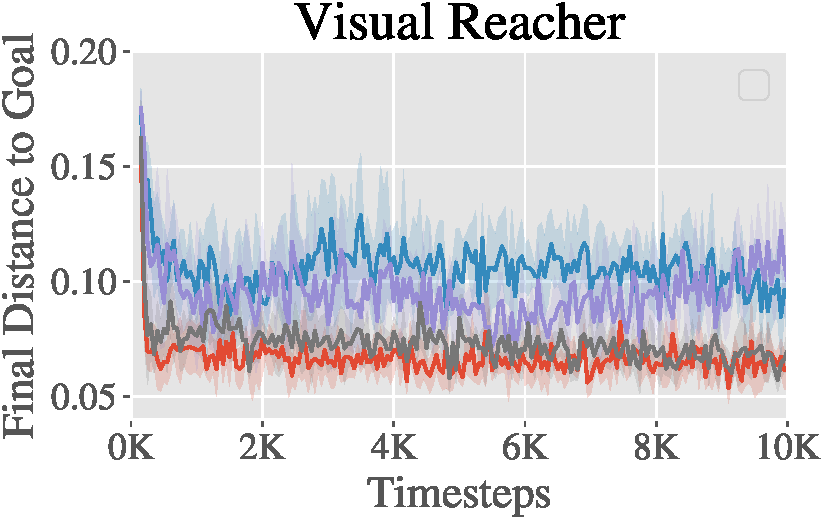
\includegraphics[height=0.185\linewidth]{img/reacher_relabeling_ablation.pdf}
    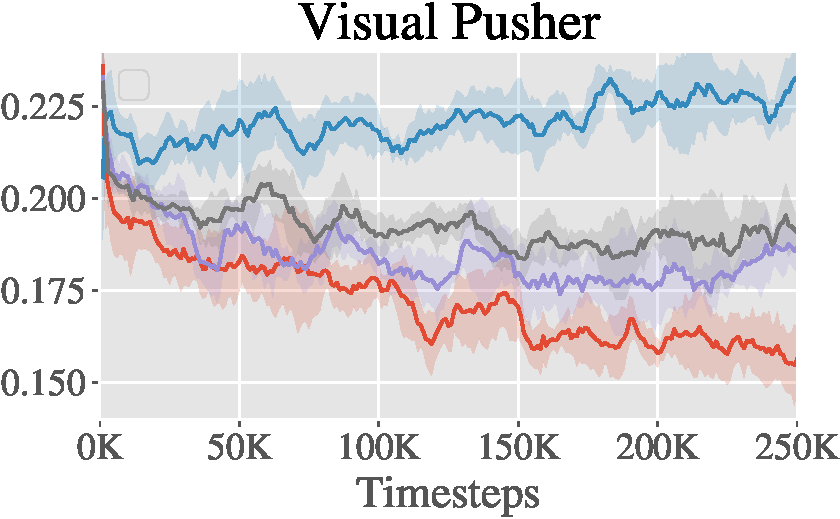
\includegraphics[height=0.185\linewidth]{img/pusher_relabeling_ablation.pdf}
    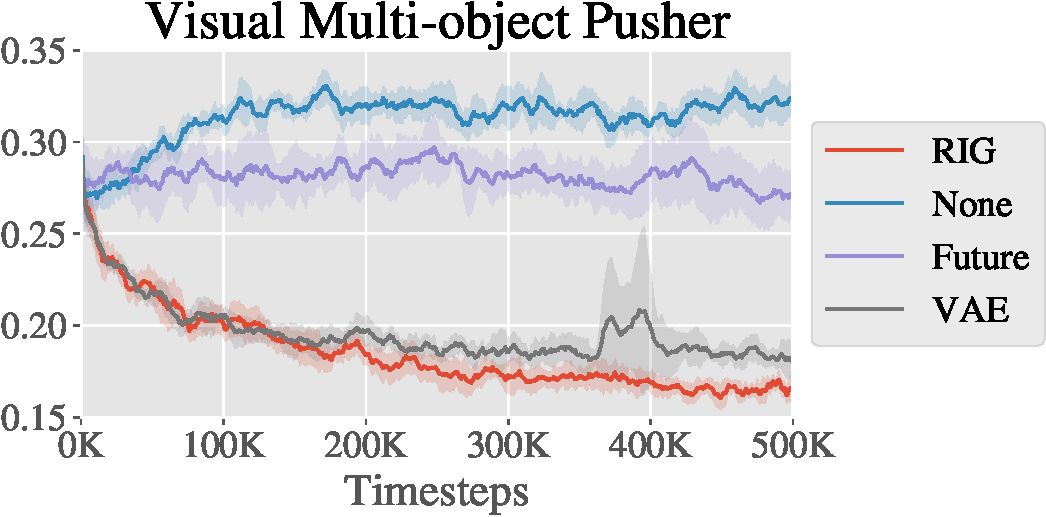
\includegraphics[height=0.185\linewidth]{img/multiobj_pusher_relabeling_ablation.pdf}
    \caption{Relabeling ablation simulated results, showing final distance to goal vs environment steps. RIG (red), which uses a mixture of VAE and future, consistently matches or outperforms the other methods.}
    \vspace{-0.1in}
    \label{fig:relabel-ablation-all-envs}
\end{figure}

\subsection{Reward type ablation}

In this experiment, we change only the reward function that we use to train the goal-conditioned valued function to show the effect of using the latent distance reward.
We include the following methods for comparison:
\textit{Latent Distance}, which is the reward used in RIG, i.e. $A = \mathbf{I}$ in Equation \eqref{eq:reward-log-prob-equivalence};
\textit{Log Probability}, which uses the Mahalanobis distance in Equation \eqref{eq:reward-log-prob-equivalence}, where $A$ is the precision matrix of the encoder;
and \textit{Pixel MSE}, which computes mean-squared error (MSE) between state and goal in pixel space. To compute the pixel MSE for a sampled latent goal, we decode the goal latent using the VAE decoder, $p_\psi$, to generate the corresponding goal image. Figure \ref{fig:reward-ablation-all-envs} shows the effect of different rewards with our method.

\begin{figure}[h]
    \centering
    % \includegraphics[height=0.25\linewidth]{img/reacher_reward_type_ablation_b.pdf}
    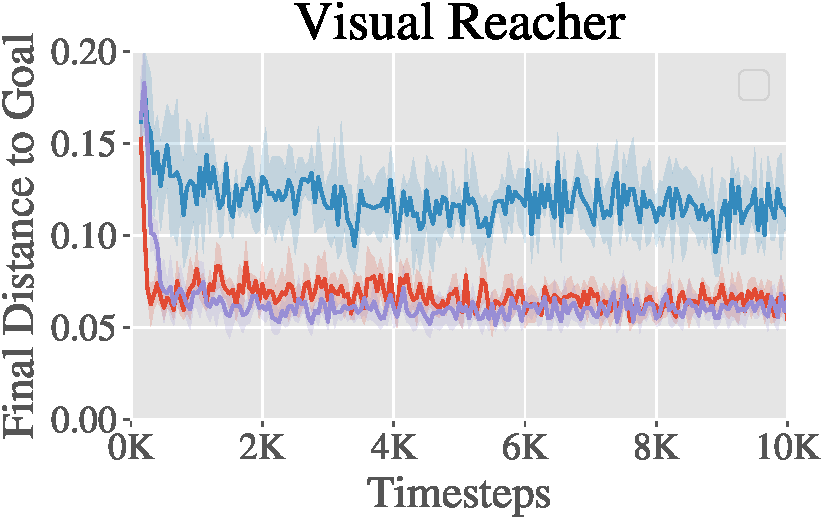
\includegraphics[height=0.19\linewidth]{img/reacher_reward_type_ablation.pdf}
    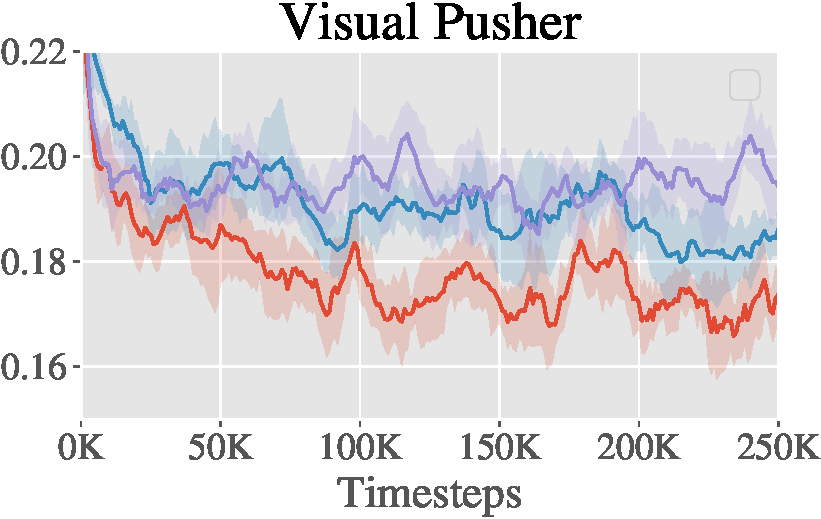
\includegraphics[height=0.19\linewidth]{img/pusher_reward_type_ablation.pdf}
    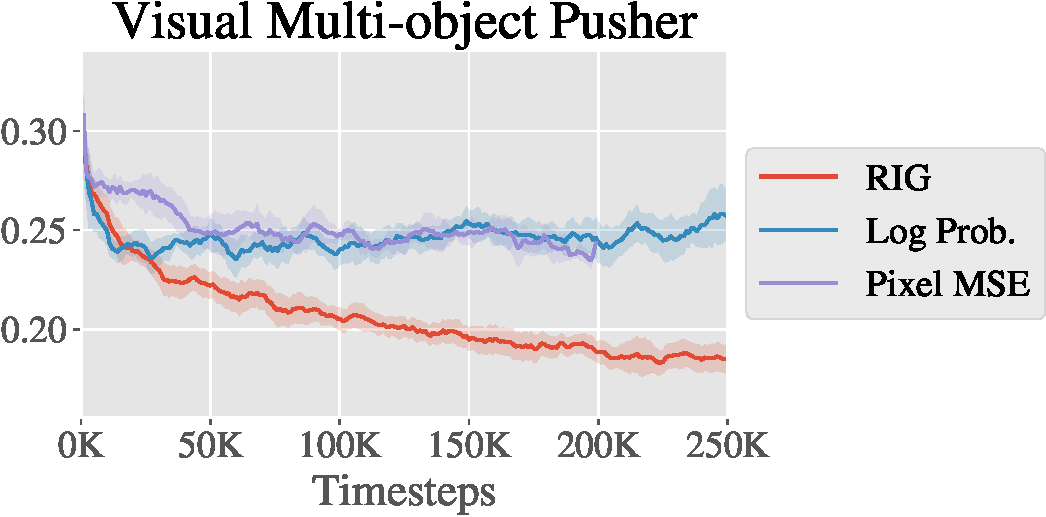
\includegraphics[height=0.19\linewidth]{img/multiobj_pusher_reward_type_ablation.pdf}
    \caption{Reward type ablation simulated results, showing final distance to goal vs environment steps. RIG (red), which uses latent distance for the reward, consistently matches or outperforms the other reward types.}
    \vspace{-0.1in}
    \label{fig:reward-ablation-all-envs}
\end{figure}

\subsection{Online training ablation} \label{sec:appendix_online}
Rather than pre-training the VAE on a set of images collected by a random policy, here we train the VAE in an online manner: the VAE is not trained when we initially collect data with our policy.
After every 3000 environment steps, we train the VAE on all of the images observed by the policy.
We show in Figure \ref{fig:online-ablation-all-envs} that this online training results in a good policy and is substantially better than leaving the VAE untrained.
These results show that the representation learning can be done simultaneously as the reinforcement learning portion of RIG, eliminating the need to have a predefined set of images to train the VAE.

The Visual Pusher experiment for this ablation is performed on a slightly easier version of the Visual Pusher used for the main results.
In particular, the goal space is reduced to be three quarters of its original size in the lateral dimension.

\begin{figure}[h]
    \centering
    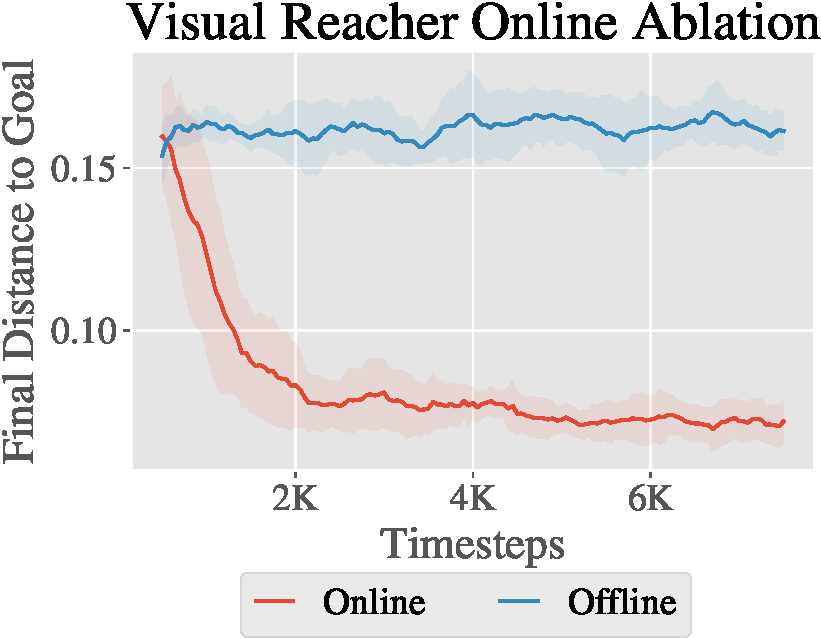
\includegraphics[height=0.2\linewidth]{img/reacher_online_ablation.pdf}
    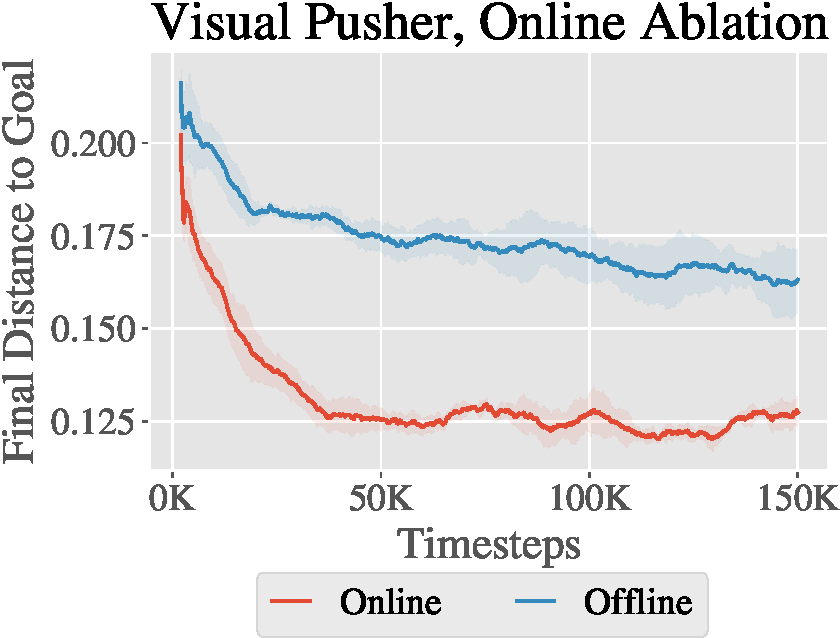
\includegraphics[height=0.2\linewidth]{img/pusher_online_ablation.pdf}
    \caption{Online vs offline VAE training ablation simulated results, showing final distance to goal vs environment steps. Given no pre-training phase, training the VAE online (red), outperforms no training of the VAE, and also performs well.}
    \vspace{-0.1in}
    \label{fig:online-ablation-all-envs}
\end{figure}

\subsection{Comparison to Hindsight Experience Replay} \label{sec:her_relabeling_ablation}

In this section, we study in isolation the effect of sampling goals from the goal space directly for Q-learning, as covered in Section~\ref{sec:goal-relabeling}.
Like hindsight experience replay \cite{andrychowicz2017her}, in this section we assume access to state information and the goal space, so we do not use a VAE.

To match the original work as closely as possible, this comparison was based off of the OpenAI baselines code \cite{plappert2018techreport} and we compare on the same Fetch robotics tasks. To minimize sample complexity and due to computational constraints, we use single threaded training with \texttt{rollout\_batch\_size=1, n\_cycles=1, batch\_size=256}. For testing, \texttt{n\_test\_rollouts=1} and the results are averaged over the last 100 test episodes. Number of updates per cycle corresponds to \texttt{n\_batches}.

On the plots, ``Future'' indicates
the future strategy as presented in \citet{andrychowicz2017her} with $k=4$. ``Ours'' indicates
resampling goals with probability 0.5 from the "future" strategy with $k=4$ and probability 0.5 uniformly from the environment goal space. Each method is shown with dense and sparse rewards.

\begin{figure}[H]
    \centering
    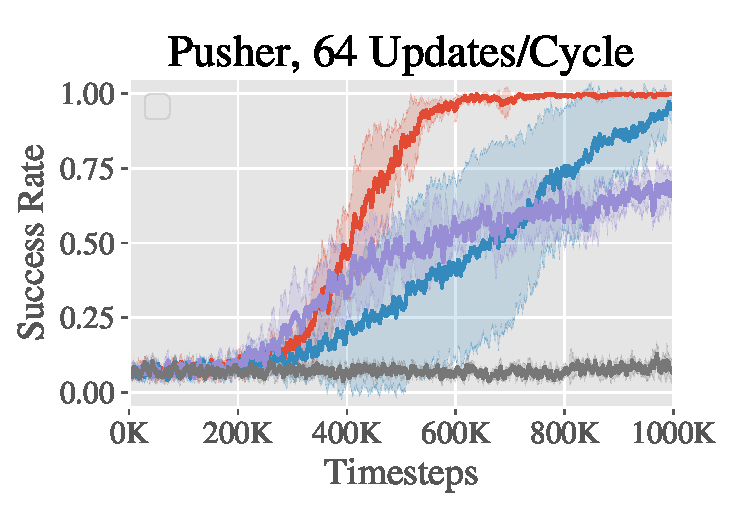
\includegraphics[height=0.2\linewidth]{img/her/push64.pdf}
    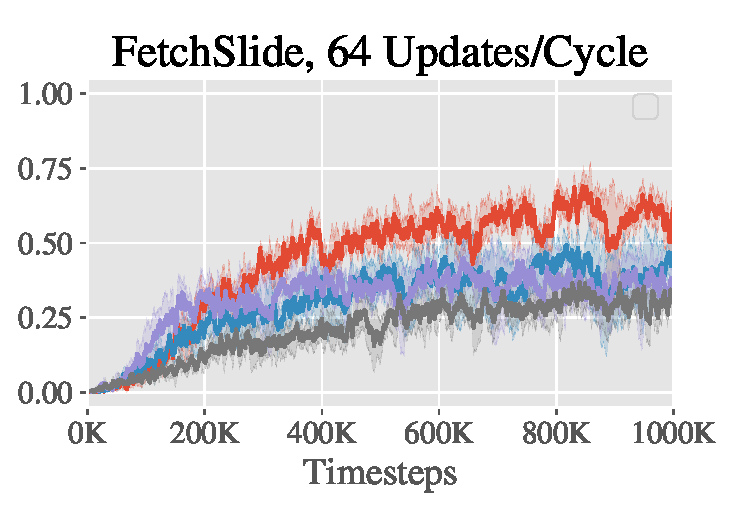
\includegraphics[height=0.2\linewidth]{img/her/slide64.pdf}
    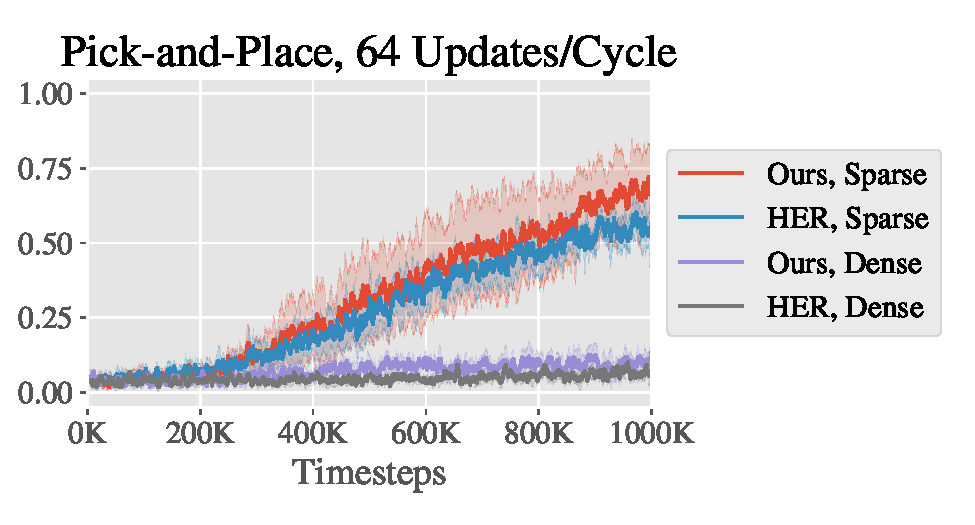
\includegraphics[height=0.2\linewidth]{img/her/pick64.pdf} \\
    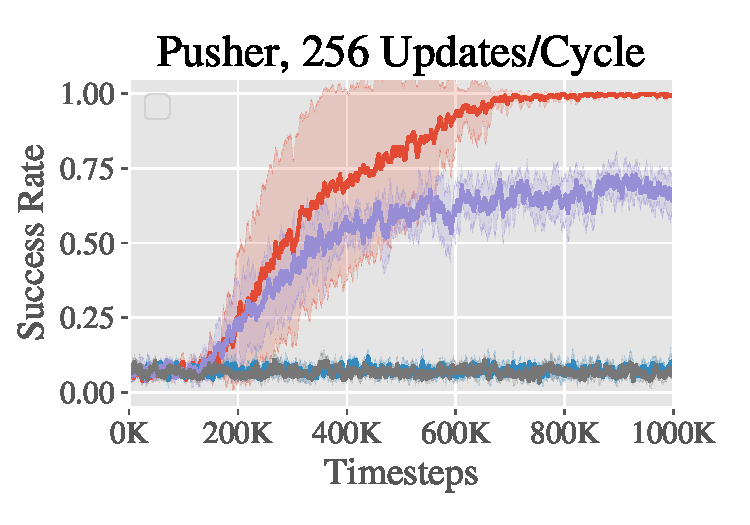
\includegraphics[height=0.2\linewidth]{img/her/push256.pdf}
    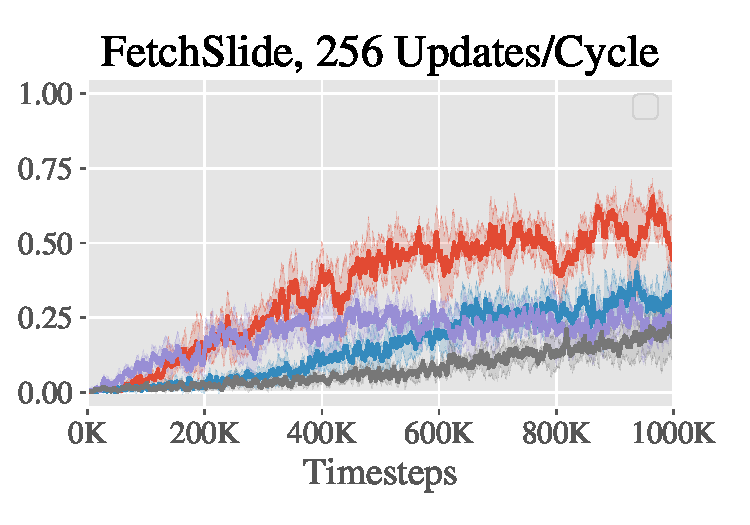
\includegraphics[height=0.2\linewidth]{img/her/slide256.pdf}
    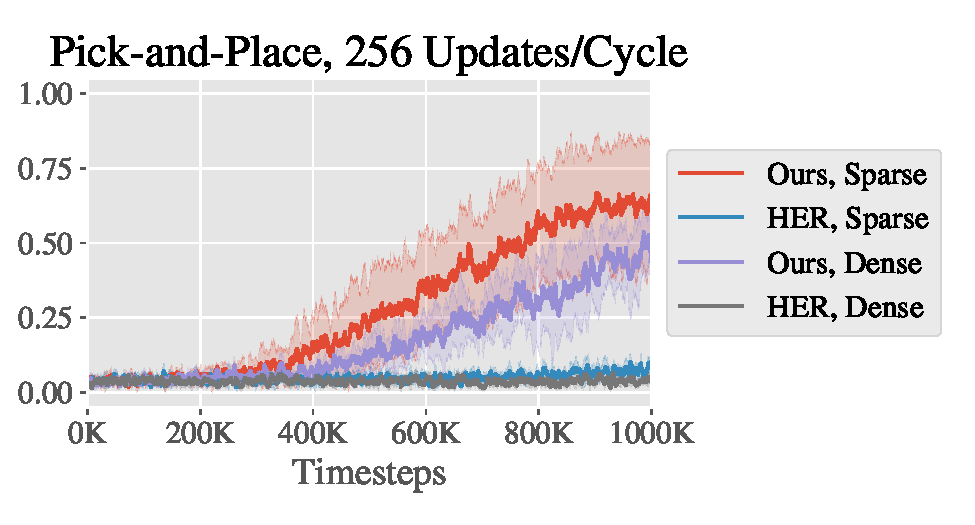
\includegraphics[height=0.2\linewidth]{img/her/pick256.pdf}
    \caption{Comparison between our relabeling strategy and HER. Each column shows a different task from the OpenAI Fetch robotics suite. The top row uses 64 gradient updates per training cycle and the bottom row uses 256 updates per cycle. Our relabeling strategy is significantly better  for both sparse and dense rewards, and for higher number of updates per cycle.}
    \vspace{-0.1in}
    \label{fig:her64}
\end{figure}

Results are shown in Figure \ref{fig:her64}. Our resampling strategy with sparse rewards consistently performs the best on the three tasks. Furthermore, it performs reasonably well with dense rewards, unlike HER alone which often fails with dense rewards. While the evaluation metric used here, success rate, is favorable to the sparse reward setting, learning with dense rewards is usually more sample efficient on most tasks and being able to do off-policy goal relabeling with dense rewards is important for RIG.

Finally, as the number of gradient updates per training cycle is increased, the performance of our strategy improves while HER does not improve and sometimes performs worse. As we apply reinforcement learning to real-world tasks, being able to reduce the required number of samples on hardware is one of the key bottlenecks. Increasing the number of gradient updates costs more compute but reduces the number of samples required to learn the tasks.

\section{Hyperparameters}
Table \ref{table:hyperparams} lists the hyperparameters used for the experiments.
\begin{table}[h]
\centering
\begin{tabular}{c|c|c}
\hline
\textbf{Hyperparameter} & \textbf{Value} & \textbf{Comments}\\
\hline
Mixture coefficient $\lambda$ & $0.5$ & See relabeling strategy ablation \\
\# training batches per time step & $4$ & Marginal improvements after $4$\\
Exploration Policy & OU, $\theta = 0.15, \sigma = 0.3$ & Outperformed Gaussian and $\epsilon$-greedy\\
$\beta$ for $\beta$-VAE & $5$ & Values around $[1, 10]$ were effective \\
Critic Learning Rate &$10^{-3}$ & Did not tune\\
Critic Regularization & None & Did not tune\\
Actor Learning Rate & $10^{-3}$ & Did not tune\\
Actor Regularization & None & Did not tune\\
Optimizer & Adam & Did not tune\\
Target Update Rate $(\tau)$ & $10^{-2}$ & Did not tune\\
Target Update Period & $2$ time steps & Did not tune\\
Target Policy Noise & $0.2$ & Did not tune\\
Target Policy Noise Clip & $0.5$ & Did not tune\\
Batch Size & $128$ & Did not tune\\
Discount Factor & $0.99$ & Did not tune\\
Reward Scaling & $10^{-4}$ & Did not tune\\
Normalized Observations & False & Did not tune\\
Gradient Clipping & False & Did not tune\\
% Critic FC sizes & False & Did not tune\\
\hline
\end{tabular}
\vspace{0.1cm}
\caption{Hyper-parameters used for all experiments.}
\label{table:hyperparams}
\end{table}

\section{Environment Details}
Below we provide a more detailed description of the simulated environments.

\textit{Visual Reacher}: A MuJoCo environment with a 7-DoF Sawyer arm reaching goal positions.
The arm is shown on the left of Figure \ref{fig:sim_screenshot} with two extra objects for the Visual Multi-Object Pusher environment (see below).
The end-effector (EE) is constrained to a 2-dimensional rectangle parallel to a table. 
The action controls EE velocity within a maximum velocity. 
The underlying state is the EE position $e$, and the underlying goal is to reach a desired EE position, $g_e$. 

\textit{Visual Pusher}: A MuJoCo environment with a 7-DoF Sawyer arm and a small puck on a table that the arm must push to a target push.
Control is the same as in Visual Reacher.
The underlying state is the EE position, $e$ and puck position $p$.
The underlying goal is for the EE to reach a desired position $g_e$ and the puck to reach a desired position $p$. 

\textit{Visual Multi-Object Pusher}: A copy of the Visual Pusher environment with two pucks.
The underlying state is the EE position, $e$ and puck positions $p_1$ and $p_2$.
The underlying goal is for the EE to reach desired position $g_e$ and the pucks to reach desired positions $g_1$ and $g_2$ respectively also constrained to each half of the workspace.
Each puck and respective goal is initialized in half of the workspace.

Videos of our method in simulated and real-world environments can be found at \url{https://sites.google.com/site/visualrlwithimaginedgoals/}.
\chapter{Appendix: Model-Based Reinforcement Learning via Meta-Policy Optimization}
\noindent\makebox[\linewidth]{\rule{\linewidth}{3.0pt}}
\begin{center}
\LARGE{\textbf{Supplementary Material}}
\end{center}
\noindent\makebox[\linewidth]{\rule{\linewidth}{0.8pt}}

\section{Complete Ablative Results} \label{sec:appendix}

\subsection{Relabeling strategy ablation} \label{sec:appendix_relabeling_ablation}

In this experiment, we compare different goal resampling strategies for training the Q function. We consider:
\textit{Future},
relabeling the goal for a transition by sampling uniformly from future states in the trajectory as done in \citet{andrychowicz2017her};
\textit{VAE}, sampling goals from the VAE only;
\textit{RIG}, relabeling goals with probability $0.5$ from the VAE and probability $0.5$ using the future strategy;
and \textit{None}, no relabeling. 
Figure \ref{fig:relabel-ablation-all-envs} shows the effect of different relabeling strategies with our method.

\begin{figure}[h]
    \centering
    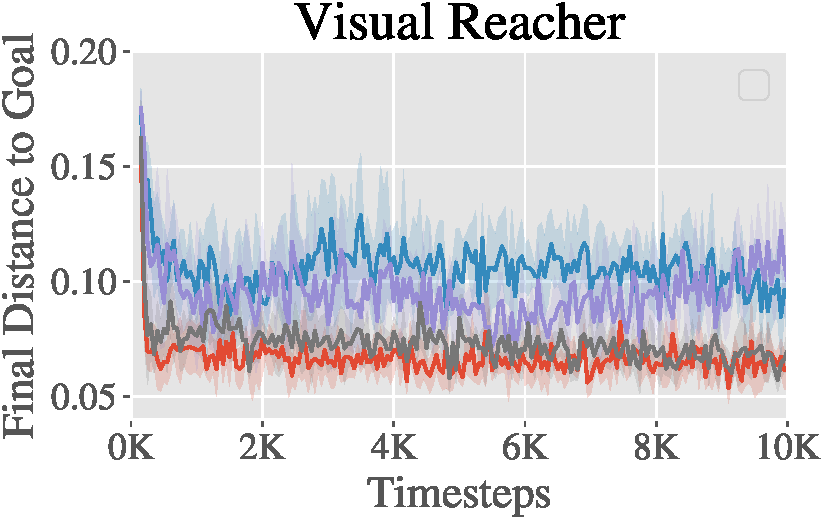
\includegraphics[height=0.185\linewidth]{img/reacher_relabeling_ablation.pdf}
    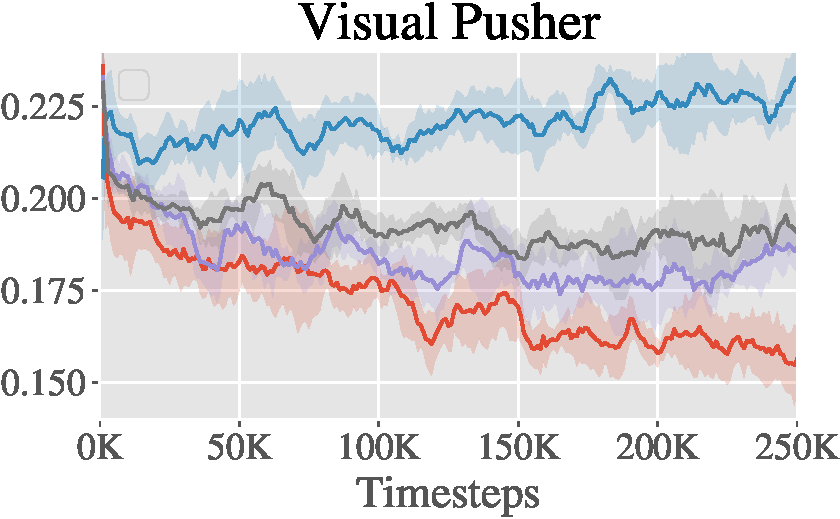
\includegraphics[height=0.185\linewidth]{img/pusher_relabeling_ablation.pdf}
    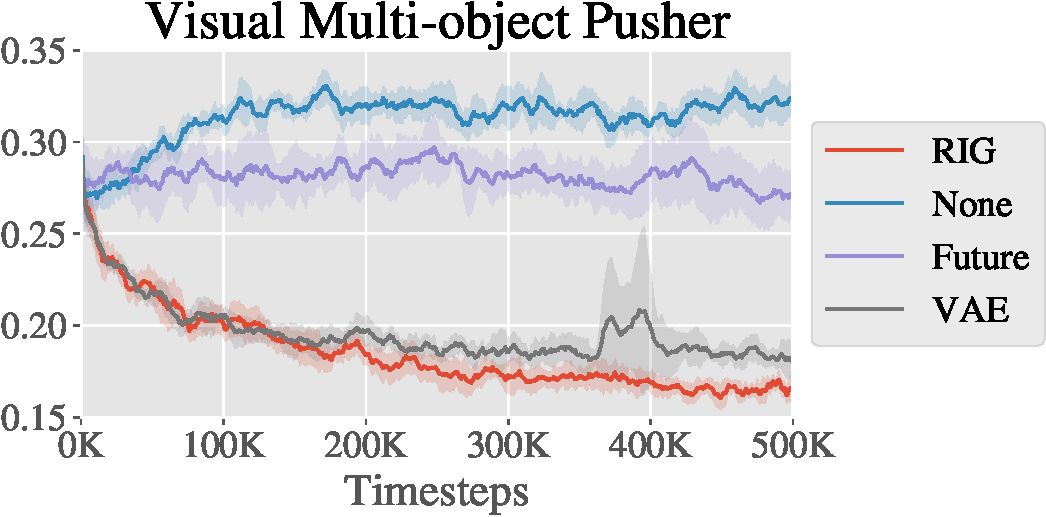
\includegraphics[height=0.185\linewidth]{img/multiobj_pusher_relabeling_ablation.pdf}
    \caption{Relabeling ablation simulated results, showing final distance to goal vs environment steps. RIG (red), which uses a mixture of VAE and future, consistently matches or outperforms the other methods.}
    \vspace{-0.1in}
    \label{fig:relabel-ablation-all-envs}
\end{figure}

\subsection{Reward type ablation}

In this experiment, we change only the reward function that we use to train the goal-conditioned valued function to show the effect of using the latent distance reward.
We include the following methods for comparison:
\textit{Latent Distance}, which is the reward used in RIG, i.e. $A = \mathbf{I}$ in Equation \eqref{eq:reward-log-prob-equivalence};
\textit{Log Probability}, which uses the Mahalanobis distance in Equation \eqref{eq:reward-log-prob-equivalence}, where $A$ is the precision matrix of the encoder;
and \textit{Pixel MSE}, which computes mean-squared error (MSE) between state and goal in pixel space. To compute the pixel MSE for a sampled latent goal, we decode the goal latent using the VAE decoder, $p_\psi$, to generate the corresponding goal image. Figure \ref{fig:reward-ablation-all-envs} shows the effect of different rewards with our method.

\begin{figure}[h]
    \centering
    % \includegraphics[height=0.25\linewidth]{img/reacher_reward_type_ablation_b.pdf}
    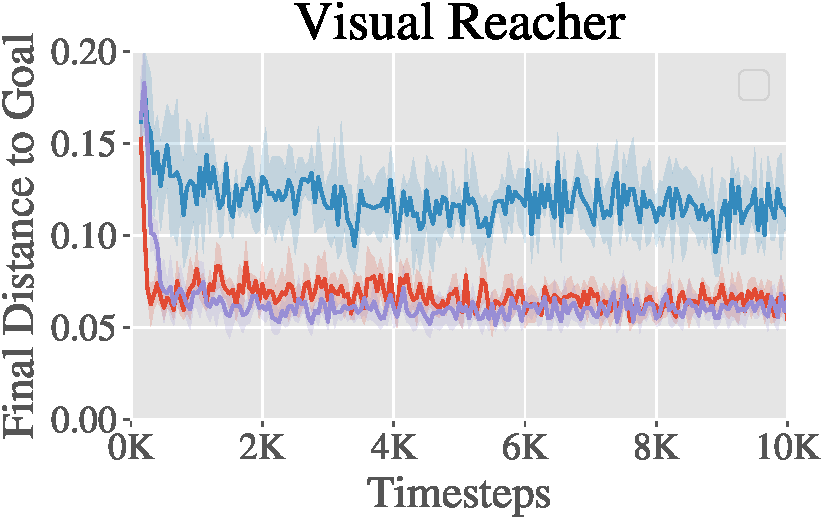
\includegraphics[height=0.19\linewidth]{img/reacher_reward_type_ablation.pdf}
    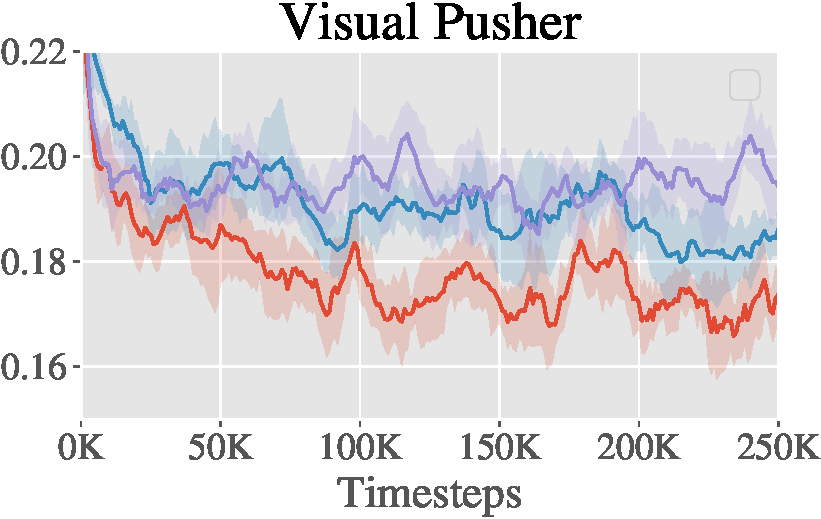
\includegraphics[height=0.19\linewidth]{img/pusher_reward_type_ablation.pdf}
    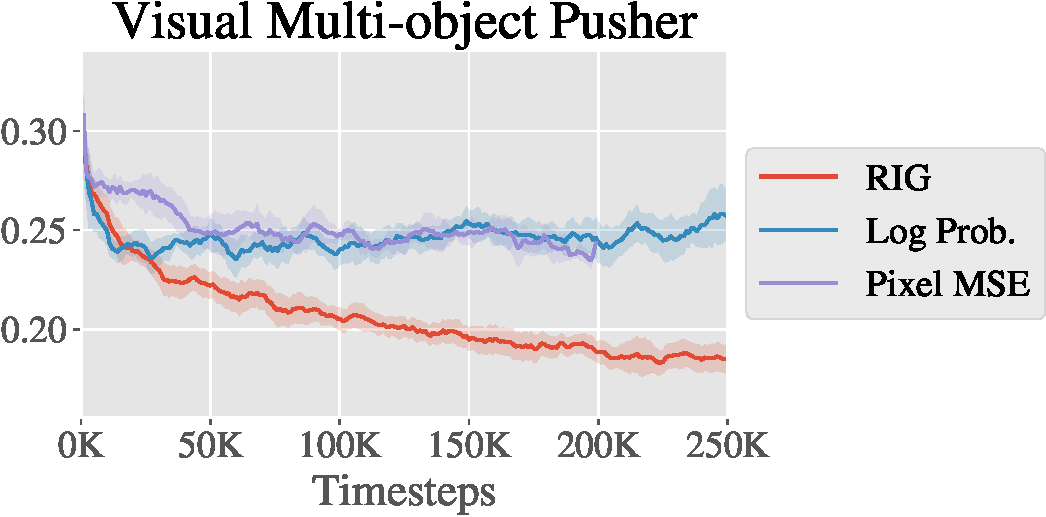
\includegraphics[height=0.19\linewidth]{img/multiobj_pusher_reward_type_ablation.pdf}
    \caption{Reward type ablation simulated results, showing final distance to goal vs environment steps. RIG (red), which uses latent distance for the reward, consistently matches or outperforms the other reward types.}
    \vspace{-0.1in}
    \label{fig:reward-ablation-all-envs}
\end{figure}

\subsection{Online training ablation} \label{sec:appendix_online}
Rather than pre-training the VAE on a set of images collected by a random policy, here we train the VAE in an online manner: the VAE is not trained when we initially collect data with our policy.
After every 3000 environment steps, we train the VAE on all of the images observed by the policy.
We show in Figure \ref{fig:online-ablation-all-envs} that this online training results in a good policy and is substantially better than leaving the VAE untrained.
These results show that the representation learning can be done simultaneously as the reinforcement learning portion of RIG, eliminating the need to have a predefined set of images to train the VAE.

The Visual Pusher experiment for this ablation is performed on a slightly easier version of the Visual Pusher used for the main results.
In particular, the goal space is reduced to be three quarters of its original size in the lateral dimension.

\begin{figure}[h]
    \centering
    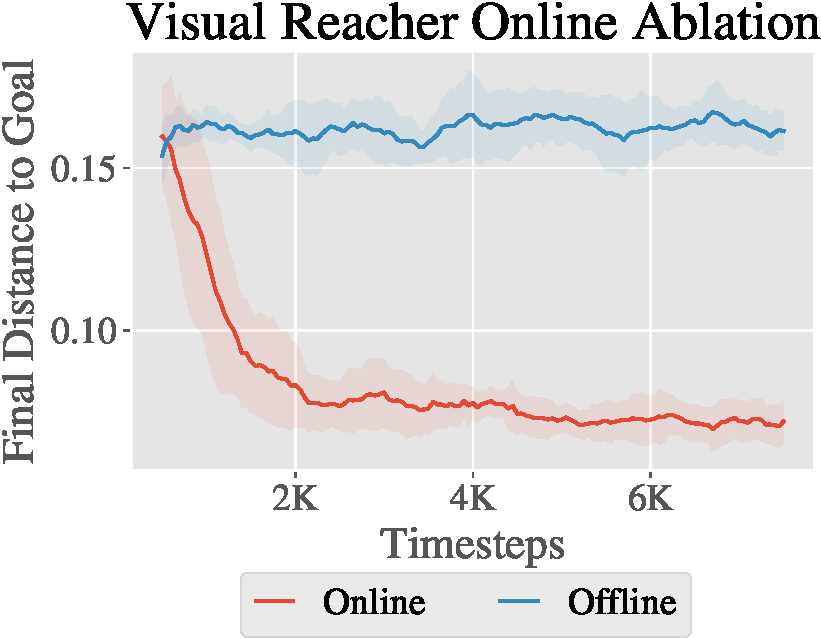
\includegraphics[height=0.2\linewidth]{img/reacher_online_ablation.pdf}
    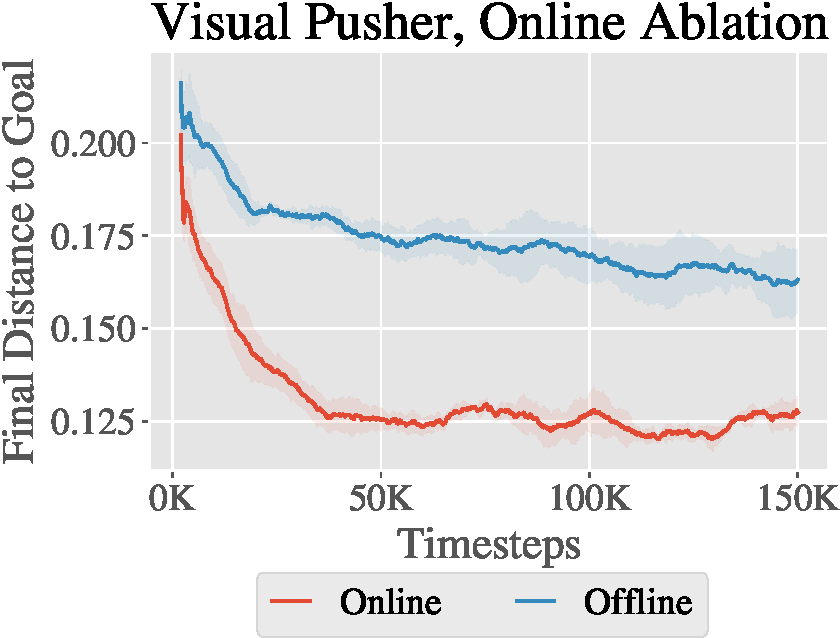
\includegraphics[height=0.2\linewidth]{img/pusher_online_ablation.pdf}
    \caption{Online vs offline VAE training ablation simulated results, showing final distance to goal vs environment steps. Given no pre-training phase, training the VAE online (red), outperforms no training of the VAE, and also performs well.}
    \vspace{-0.1in}
    \label{fig:online-ablation-all-envs}
\end{figure}

\subsection{Comparison to Hindsight Experience Replay} \label{sec:her_relabeling_ablation}

In this section, we study in isolation the effect of sampling goals from the goal space directly for Q-learning, as covered in Section~\ref{sec:goal-relabeling}.
Like hindsight experience replay \cite{andrychowicz2017her}, in this section we assume access to state information and the goal space, so we do not use a VAE.

To match the original work as closely as possible, this comparison was based off of the OpenAI baselines code \cite{plappert2018techreport} and we compare on the same Fetch robotics tasks. To minimize sample complexity and due to computational constraints, we use single threaded training with \texttt{rollout\_batch\_size=1, n\_cycles=1, batch\_size=256}. For testing, \texttt{n\_test\_rollouts=1} and the results are averaged over the last 100 test episodes. Number of updates per cycle corresponds to \texttt{n\_batches}.

On the plots, ``Future'' indicates
the future strategy as presented in \citet{andrychowicz2017her} with $k=4$. ``Ours'' indicates
resampling goals with probability 0.5 from the "future" strategy with $k=4$ and probability 0.5 uniformly from the environment goal space. Each method is shown with dense and sparse rewards.

\begin{figure}[H]
    \centering
    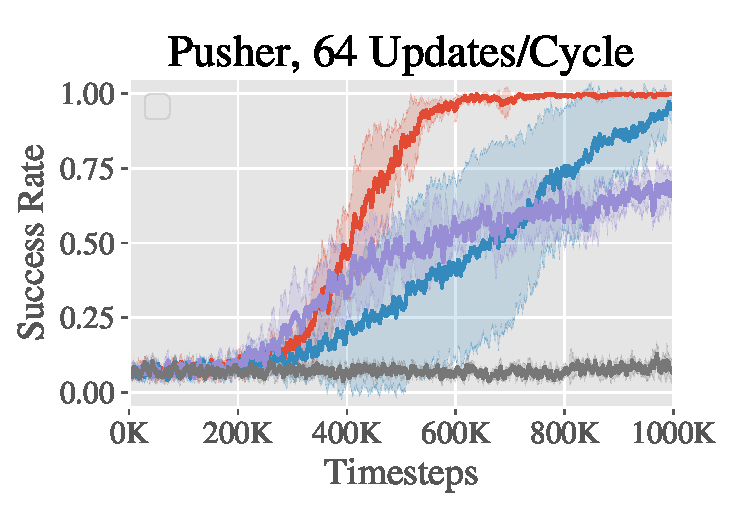
\includegraphics[height=0.2\linewidth]{img/her/push64.pdf}
    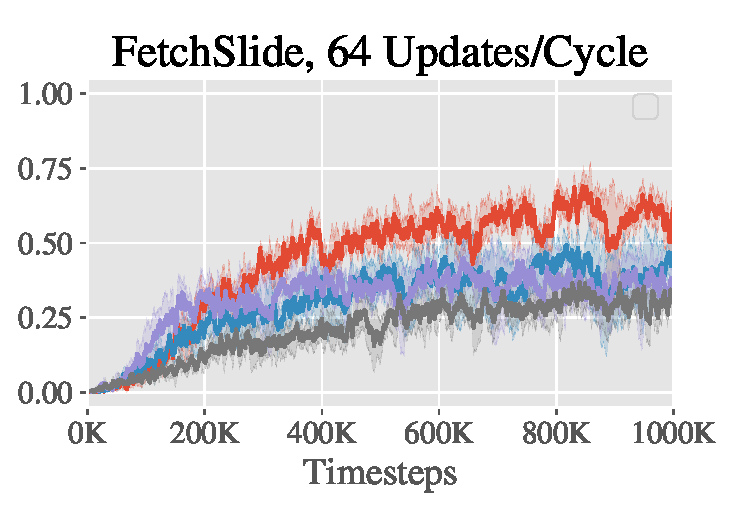
\includegraphics[height=0.2\linewidth]{img/her/slide64.pdf}
    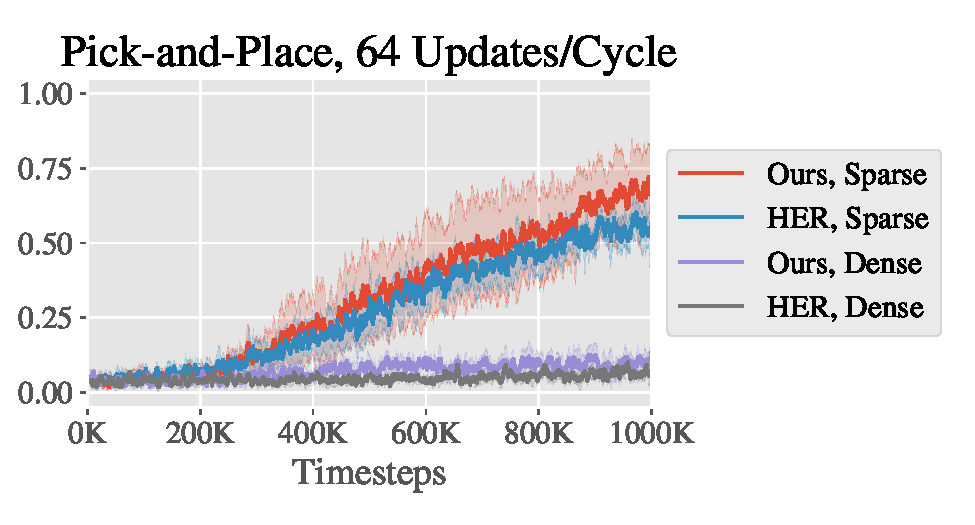
\includegraphics[height=0.2\linewidth]{img/her/pick64.pdf} \\
    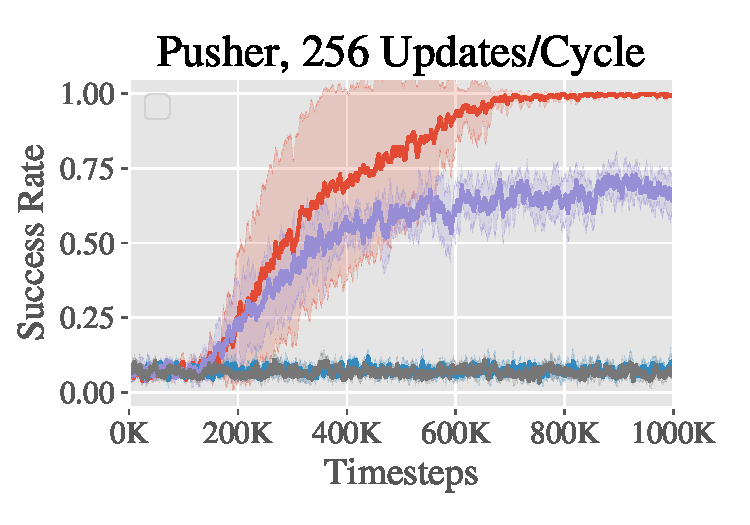
\includegraphics[height=0.2\linewidth]{img/her/push256.pdf}
    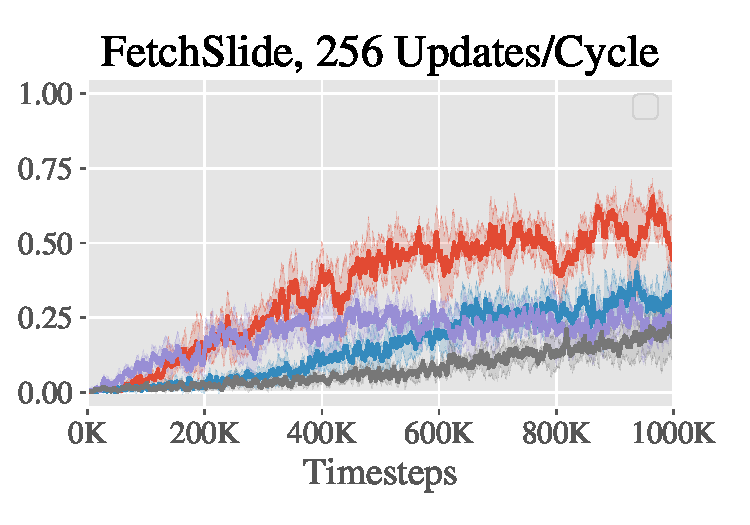
\includegraphics[height=0.2\linewidth]{img/her/slide256.pdf}
    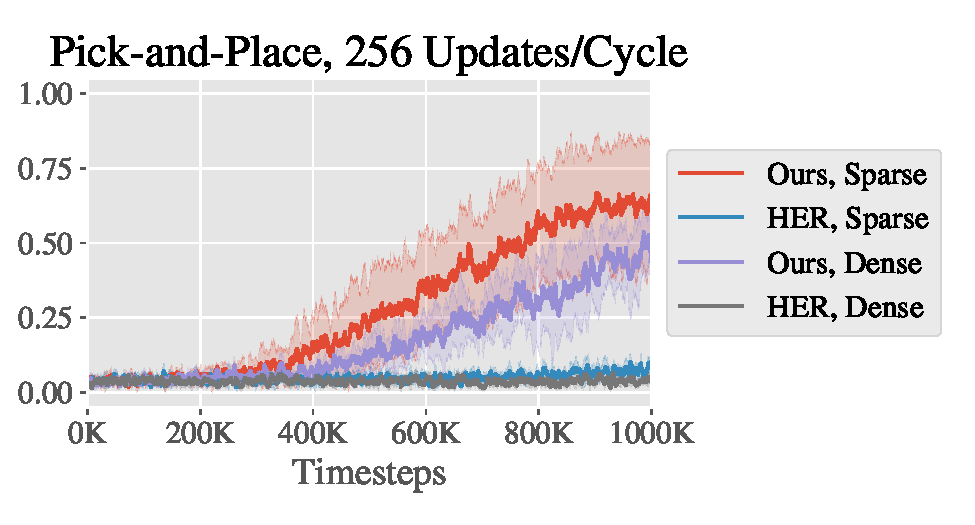
\includegraphics[height=0.2\linewidth]{img/her/pick256.pdf}
    \caption{Comparison between our relabeling strategy and HER. Each column shows a different task from the OpenAI Fetch robotics suite. The top row uses 64 gradient updates per training cycle and the bottom row uses 256 updates per cycle. Our relabeling strategy is significantly better  for both sparse and dense rewards, and for higher number of updates per cycle.}
    \vspace{-0.1in}
    \label{fig:her64}
\end{figure}

Results are shown in Figure \ref{fig:her64}. Our resampling strategy with sparse rewards consistently performs the best on the three tasks. Furthermore, it performs reasonably well with dense rewards, unlike HER alone which often fails with dense rewards. While the evaluation metric used here, success rate, is favorable to the sparse reward setting, learning with dense rewards is usually more sample efficient on most tasks and being able to do off-policy goal relabeling with dense rewards is important for RIG.

Finally, as the number of gradient updates per training cycle is increased, the performance of our strategy improves while HER does not improve and sometimes performs worse. As we apply reinforcement learning to real-world tasks, being able to reduce the required number of samples on hardware is one of the key bottlenecks. Increasing the number of gradient updates costs more compute but reduces the number of samples required to learn the tasks.

\section{Hyperparameters}
Table \ref{table:hyperparams} lists the hyperparameters used for the experiments.
\begin{table}[h]
\centering
\begin{tabular}{c|c|c}
\hline
\textbf{Hyperparameter} & \textbf{Value} & \textbf{Comments}\\
\hline
Mixture coefficient $\lambda$ & $0.5$ & See relabeling strategy ablation \\
\# training batches per time step & $4$ & Marginal improvements after $4$\\
Exploration Policy & OU, $\theta = 0.15, \sigma = 0.3$ & Outperformed Gaussian and $\epsilon$-greedy\\
$\beta$ for $\beta$-VAE & $5$ & Values around $[1, 10]$ were effective \\
Critic Learning Rate &$10^{-3}$ & Did not tune\\
Critic Regularization & None & Did not tune\\
Actor Learning Rate & $10^{-3}$ & Did not tune\\
Actor Regularization & None & Did not tune\\
Optimizer & Adam & Did not tune\\
Target Update Rate $(\tau)$ & $10^{-2}$ & Did not tune\\
Target Update Period & $2$ time steps & Did not tune\\
Target Policy Noise & $0.2$ & Did not tune\\
Target Policy Noise Clip & $0.5$ & Did not tune\\
Batch Size & $128$ & Did not tune\\
Discount Factor & $0.99$ & Did not tune\\
Reward Scaling & $10^{-4}$ & Did not tune\\
Normalized Observations & False & Did not tune\\
Gradient Clipping & False & Did not tune\\
% Critic FC sizes & False & Did not tune\\
\hline
\end{tabular}
\vspace{0.1cm}
\caption{Hyper-parameters used for all experiments.}
\label{table:hyperparams}
\end{table}

\section{Environment Details}
Below we provide a more detailed description of the simulated environments.

\textit{Visual Reacher}: A MuJoCo environment with a 7-DoF Sawyer arm reaching goal positions.
The arm is shown on the left of Figure \ref{fig:sim_screenshot} with two extra objects for the Visual Multi-Object Pusher environment (see below).
The end-effector (EE) is constrained to a 2-dimensional rectangle parallel to a table. 
The action controls EE velocity within a maximum velocity. 
The underlying state is the EE position $e$, and the underlying goal is to reach a desired EE position, $g_e$. 

\textit{Visual Pusher}: A MuJoCo environment with a 7-DoF Sawyer arm and a small puck on a table that the arm must push to a target push.
Control is the same as in Visual Reacher.
The underlying state is the EE position, $e$ and puck position $p$.
The underlying goal is for the EE to reach a desired position $g_e$ and the puck to reach a desired position $p$. 

\textit{Visual Multi-Object Pusher}: A copy of the Visual Pusher environment with two pucks.
The underlying state is the EE position, $e$ and puck positions $p_1$ and $p_2$.
The underlying goal is for the EE to reach desired position $g_e$ and the pucks to reach desired positions $g_1$ and $g_2$ respectively also constrained to each half of the workspace.
Each puck and respective goal is initialized in half of the workspace.

Videos of our method in simulated and real-world environments can be found at \url{https://sites.google.com/site/visualrlwithimaginedgoals/}.
\chapter{Appendix: ProMP: Proximal Meta-Policy Search}
\noindent\makebox[\linewidth]{\rule{\linewidth}{3.0pt}}
\begin{center}
\LARGE{\textbf{Supplementary Material}}
\end{center}
\noindent\makebox[\linewidth]{\rule{\linewidth}{0.8pt}}

\section{Complete Ablative Results} \label{sec:appendix}

\subsection{Relabeling strategy ablation} \label{sec:appendix_relabeling_ablation}

In this experiment, we compare different goal resampling strategies for training the Q function. We consider:
\textit{Future},
relabeling the goal for a transition by sampling uniformly from future states in the trajectory as done in \citet{andrychowicz2017her};
\textit{VAE}, sampling goals from the VAE only;
\textit{RIG}, relabeling goals with probability $0.5$ from the VAE and probability $0.5$ using the future strategy;
and \textit{None}, no relabeling. 
Figure \ref{fig:relabel-ablation-all-envs} shows the effect of different relabeling strategies with our method.

\begin{figure}[h]
    \centering
    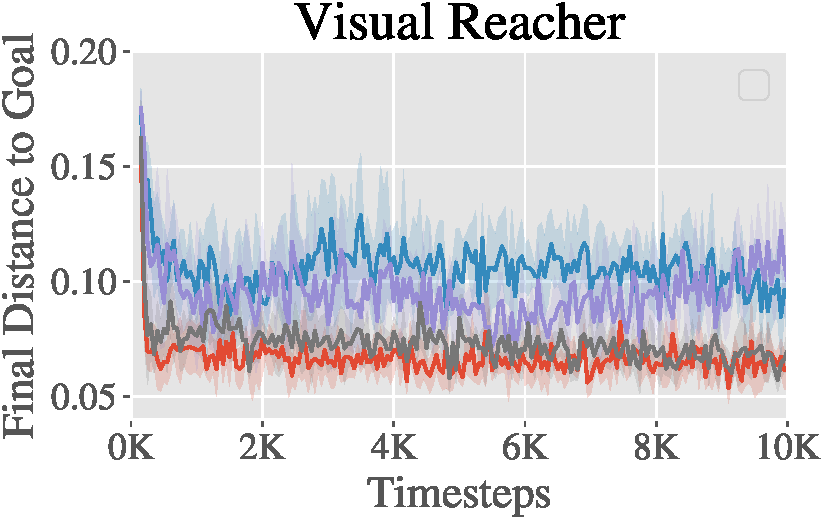
\includegraphics[height=0.185\linewidth]{img/reacher_relabeling_ablation.pdf}
    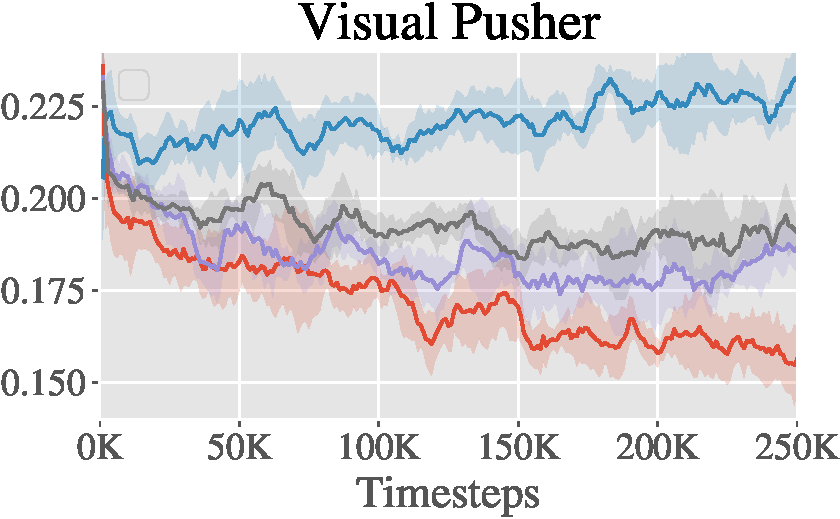
\includegraphics[height=0.185\linewidth]{img/pusher_relabeling_ablation.pdf}
    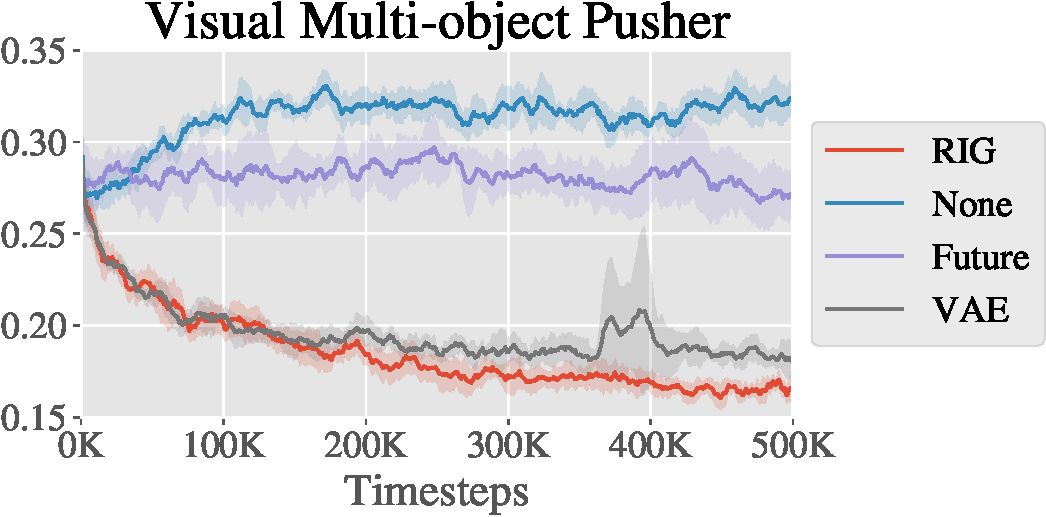
\includegraphics[height=0.185\linewidth]{img/multiobj_pusher_relabeling_ablation.pdf}
    \caption{Relabeling ablation simulated results, showing final distance to goal vs environment steps. RIG (red), which uses a mixture of VAE and future, consistently matches or outperforms the other methods.}
    \vspace{-0.1in}
    \label{fig:relabel-ablation-all-envs}
\end{figure}

\subsection{Reward type ablation}

In this experiment, we change only the reward function that we use to train the goal-conditioned valued function to show the effect of using the latent distance reward.
We include the following methods for comparison:
\textit{Latent Distance}, which is the reward used in RIG, i.e. $A = \mathbf{I}$ in Equation \eqref{eq:reward-log-prob-equivalence};
\textit{Log Probability}, which uses the Mahalanobis distance in Equation \eqref{eq:reward-log-prob-equivalence}, where $A$ is the precision matrix of the encoder;
and \textit{Pixel MSE}, which computes mean-squared error (MSE) between state and goal in pixel space. To compute the pixel MSE for a sampled latent goal, we decode the goal latent using the VAE decoder, $p_\psi$, to generate the corresponding goal image. Figure \ref{fig:reward-ablation-all-envs} shows the effect of different rewards with our method.

\begin{figure}[h]
    \centering
    % \includegraphics[height=0.25\linewidth]{img/reacher_reward_type_ablation_b.pdf}
    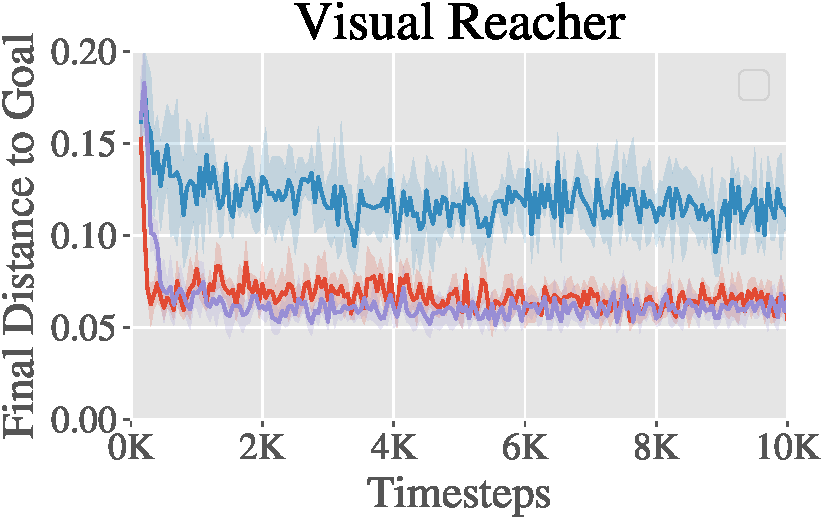
\includegraphics[height=0.19\linewidth]{img/reacher_reward_type_ablation.pdf}
    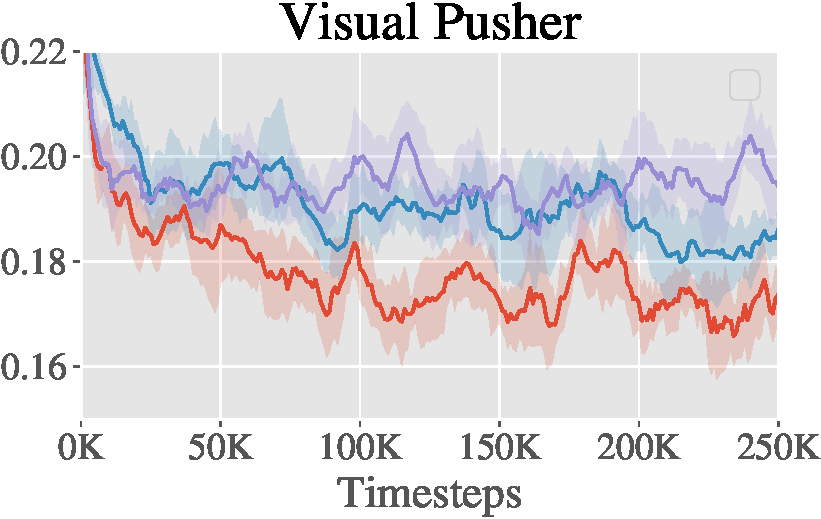
\includegraphics[height=0.19\linewidth]{img/pusher_reward_type_ablation.pdf}
    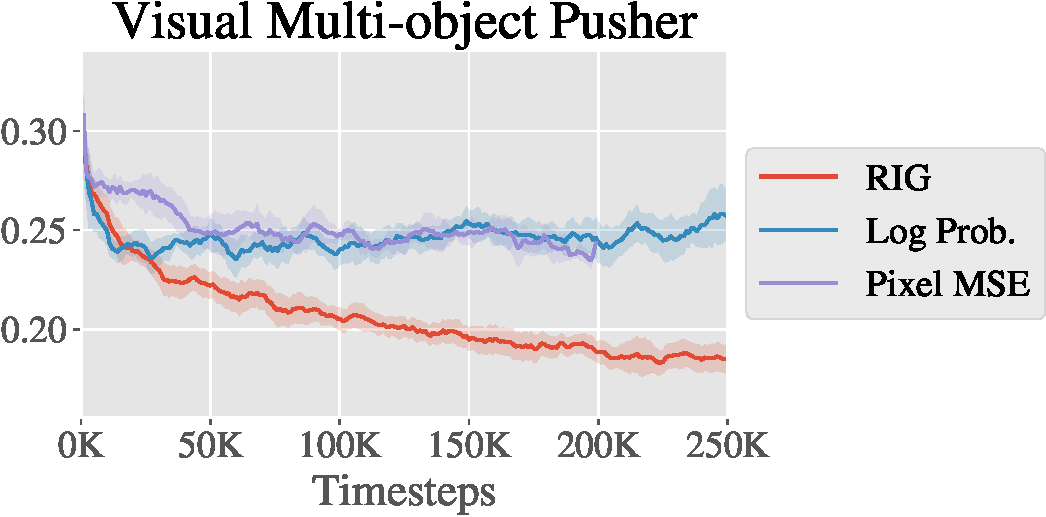
\includegraphics[height=0.19\linewidth]{img/multiobj_pusher_reward_type_ablation.pdf}
    \caption{Reward type ablation simulated results, showing final distance to goal vs environment steps. RIG (red), which uses latent distance for the reward, consistently matches or outperforms the other reward types.}
    \vspace{-0.1in}
    \label{fig:reward-ablation-all-envs}
\end{figure}

\subsection{Online training ablation} \label{sec:appendix_online}
Rather than pre-training the VAE on a set of images collected by a random policy, here we train the VAE in an online manner: the VAE is not trained when we initially collect data with our policy.
After every 3000 environment steps, we train the VAE on all of the images observed by the policy.
We show in Figure \ref{fig:online-ablation-all-envs} that this online training results in a good policy and is substantially better than leaving the VAE untrained.
These results show that the representation learning can be done simultaneously as the reinforcement learning portion of RIG, eliminating the need to have a predefined set of images to train the VAE.

The Visual Pusher experiment for this ablation is performed on a slightly easier version of the Visual Pusher used for the main results.
In particular, the goal space is reduced to be three quarters of its original size in the lateral dimension.

\begin{figure}[h]
    \centering
    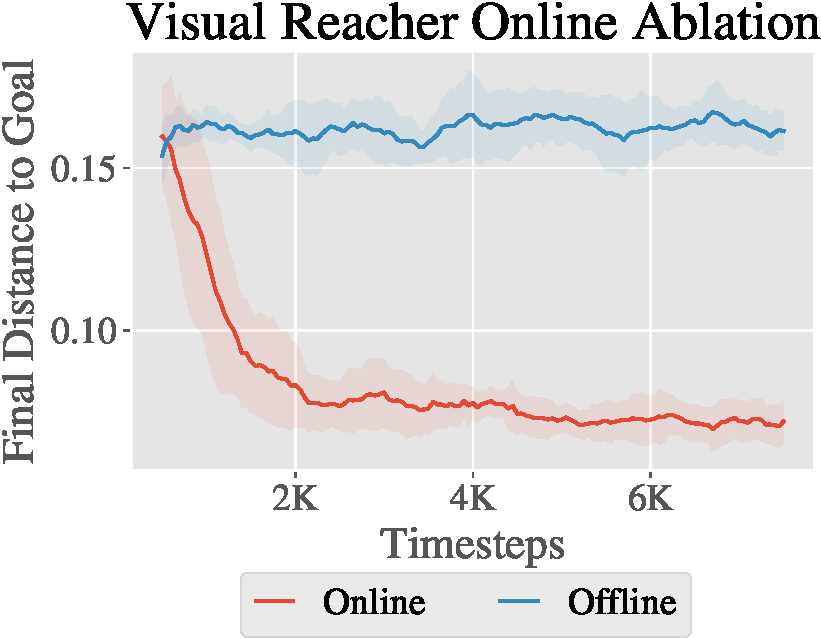
\includegraphics[height=0.2\linewidth]{img/reacher_online_ablation.pdf}
    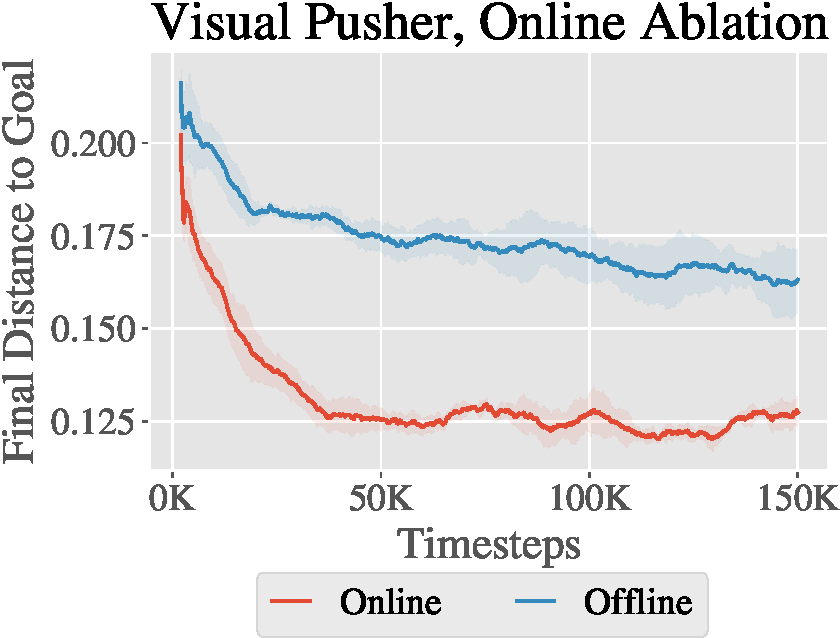
\includegraphics[height=0.2\linewidth]{img/pusher_online_ablation.pdf}
    \caption{Online vs offline VAE training ablation simulated results, showing final distance to goal vs environment steps. Given no pre-training phase, training the VAE online (red), outperforms no training of the VAE, and also performs well.}
    \vspace{-0.1in}
    \label{fig:online-ablation-all-envs}
\end{figure}

\subsection{Comparison to Hindsight Experience Replay} \label{sec:her_relabeling_ablation}

In this section, we study in isolation the effect of sampling goals from the goal space directly for Q-learning, as covered in Section~\ref{sec:goal-relabeling}.
Like hindsight experience replay \cite{andrychowicz2017her}, in this section we assume access to state information and the goal space, so we do not use a VAE.

To match the original work as closely as possible, this comparison was based off of the OpenAI baselines code \cite{plappert2018techreport} and we compare on the same Fetch robotics tasks. To minimize sample complexity and due to computational constraints, we use single threaded training with \texttt{rollout\_batch\_size=1, n\_cycles=1, batch\_size=256}. For testing, \texttt{n\_test\_rollouts=1} and the results are averaged over the last 100 test episodes. Number of updates per cycle corresponds to \texttt{n\_batches}.

On the plots, ``Future'' indicates
the future strategy as presented in \citet{andrychowicz2017her} with $k=4$. ``Ours'' indicates
resampling goals with probability 0.5 from the "future" strategy with $k=4$ and probability 0.5 uniformly from the environment goal space. Each method is shown with dense and sparse rewards.

\begin{figure}[H]
    \centering
    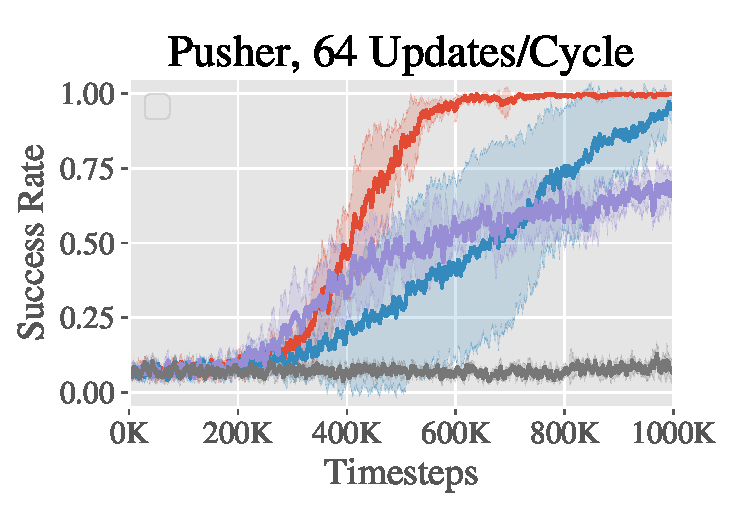
\includegraphics[height=0.2\linewidth]{img/her/push64.pdf}
    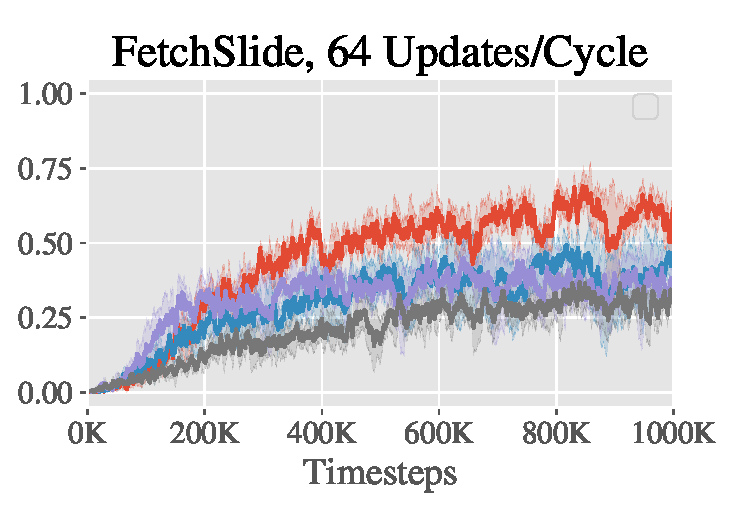
\includegraphics[height=0.2\linewidth]{img/her/slide64.pdf}
    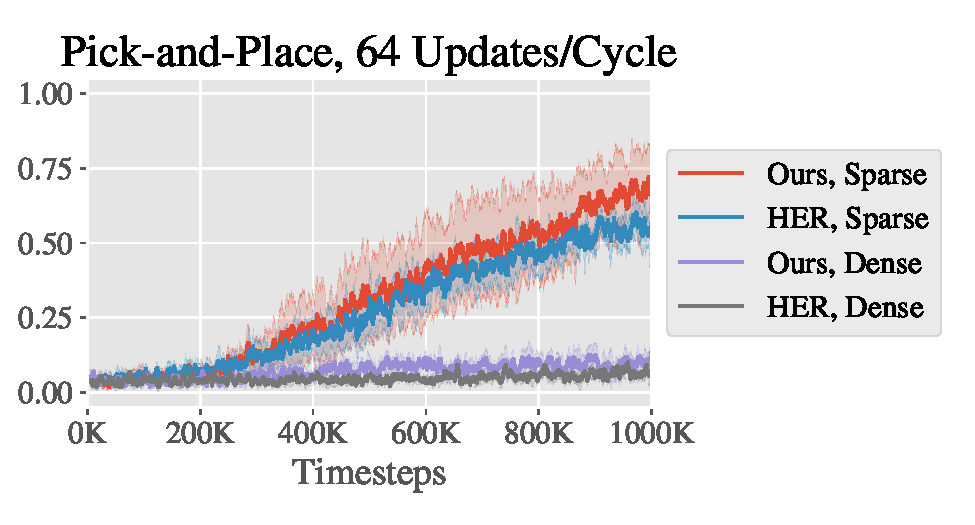
\includegraphics[height=0.2\linewidth]{img/her/pick64.pdf} \\
    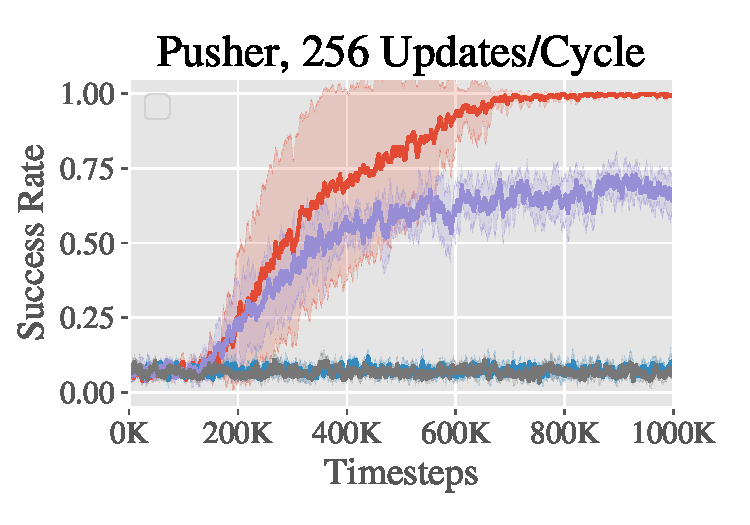
\includegraphics[height=0.2\linewidth]{img/her/push256.pdf}
    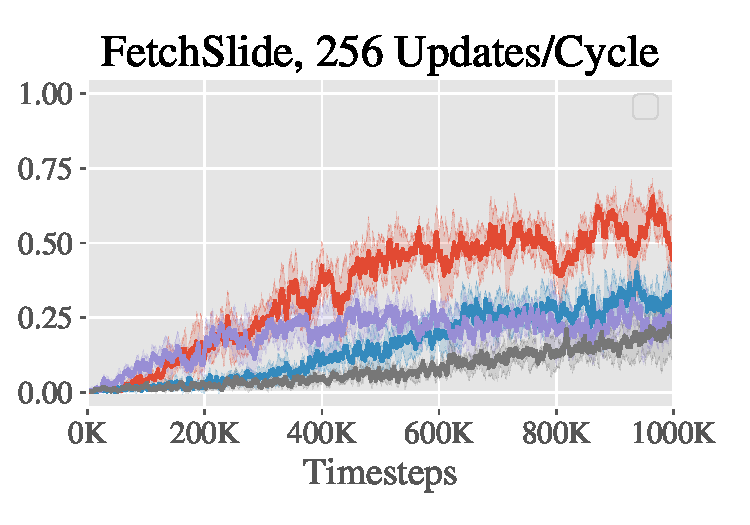
\includegraphics[height=0.2\linewidth]{img/her/slide256.pdf}
    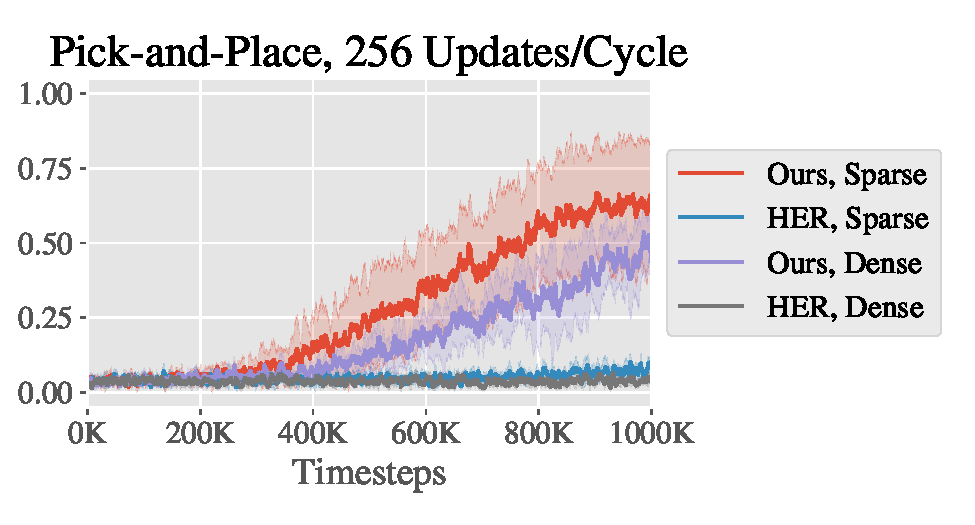
\includegraphics[height=0.2\linewidth]{img/her/pick256.pdf}
    \caption{Comparison between our relabeling strategy and HER. Each column shows a different task from the OpenAI Fetch robotics suite. The top row uses 64 gradient updates per training cycle and the bottom row uses 256 updates per cycle. Our relabeling strategy is significantly better  for both sparse and dense rewards, and for higher number of updates per cycle.}
    \vspace{-0.1in}
    \label{fig:her64}
\end{figure}

Results are shown in Figure \ref{fig:her64}. Our resampling strategy with sparse rewards consistently performs the best on the three tasks. Furthermore, it performs reasonably well with dense rewards, unlike HER alone which often fails with dense rewards. While the evaluation metric used here, success rate, is favorable to the sparse reward setting, learning with dense rewards is usually more sample efficient on most tasks and being able to do off-policy goal relabeling with dense rewards is important for RIG.

Finally, as the number of gradient updates per training cycle is increased, the performance of our strategy improves while HER does not improve and sometimes performs worse. As we apply reinforcement learning to real-world tasks, being able to reduce the required number of samples on hardware is one of the key bottlenecks. Increasing the number of gradient updates costs more compute but reduces the number of samples required to learn the tasks.

\section{Hyperparameters}
Table \ref{table:hyperparams} lists the hyperparameters used for the experiments.
\begin{table}[h]
\centering
\begin{tabular}{c|c|c}
\hline
\textbf{Hyperparameter} & \textbf{Value} & \textbf{Comments}\\
\hline
Mixture coefficient $\lambda$ & $0.5$ & See relabeling strategy ablation \\
\# training batches per time step & $4$ & Marginal improvements after $4$\\
Exploration Policy & OU, $\theta = 0.15, \sigma = 0.3$ & Outperformed Gaussian and $\epsilon$-greedy\\
$\beta$ for $\beta$-VAE & $5$ & Values around $[1, 10]$ were effective \\
Critic Learning Rate &$10^{-3}$ & Did not tune\\
Critic Regularization & None & Did not tune\\
Actor Learning Rate & $10^{-3}$ & Did not tune\\
Actor Regularization & None & Did not tune\\
Optimizer & Adam & Did not tune\\
Target Update Rate $(\tau)$ & $10^{-2}$ & Did not tune\\
Target Update Period & $2$ time steps & Did not tune\\
Target Policy Noise & $0.2$ & Did not tune\\
Target Policy Noise Clip & $0.5$ & Did not tune\\
Batch Size & $128$ & Did not tune\\
Discount Factor & $0.99$ & Did not tune\\
Reward Scaling & $10^{-4}$ & Did not tune\\
Normalized Observations & False & Did not tune\\
Gradient Clipping & False & Did not tune\\
% Critic FC sizes & False & Did not tune\\
\hline
\end{tabular}
\vspace{0.1cm}
\caption{Hyper-parameters used for all experiments.}
\label{table:hyperparams}
\end{table}

\section{Environment Details}
Below we provide a more detailed description of the simulated environments.

\textit{Visual Reacher}: A MuJoCo environment with a 7-DoF Sawyer arm reaching goal positions.
The arm is shown on the left of Figure \ref{fig:sim_screenshot} with two extra objects for the Visual Multi-Object Pusher environment (see below).
The end-effector (EE) is constrained to a 2-dimensional rectangle parallel to a table. 
The action controls EE velocity within a maximum velocity. 
The underlying state is the EE position $e$, and the underlying goal is to reach a desired EE position, $g_e$. 

\textit{Visual Pusher}: A MuJoCo environment with a 7-DoF Sawyer arm and a small puck on a table that the arm must push to a target push.
Control is the same as in Visual Reacher.
The underlying state is the EE position, $e$ and puck position $p$.
The underlying goal is for the EE to reach a desired position $g_e$ and the puck to reach a desired position $p$. 

\textit{Visual Multi-Object Pusher}: A copy of the Visual Pusher environment with two pucks.
The underlying state is the EE position, $e$ and puck positions $p_1$ and $p_2$.
The underlying goal is for the EE to reach desired position $g_e$ and the pucks to reach desired positions $g_1$ and $g_2$ respectively also constrained to each half of the workspace.
Each puck and respective goal is initialized in half of the workspace.

Videos of our method in simulated and real-world environments can be found at \url{https://sites.google.com/site/visualrlwithimaginedgoals/}.
\chapter{Appendix: Improving Model-Based Reinforcement Learning via Model-Augmented Pathwise Derivative}
\noindent\makebox[\linewidth]{\rule{\linewidth}{3.0pt}}
\begin{center}
\LARGE{\textbf{Supplementary Material}}
\end{center}
\noindent\makebox[\linewidth]{\rule{\linewidth}{0.8pt}}

\section{Complete Ablative Results} \label{sec:appendix}

\subsection{Relabeling strategy ablation} \label{sec:appendix_relabeling_ablation}

In this experiment, we compare different goal resampling strategies for training the Q function. We consider:
\textit{Future},
relabeling the goal for a transition by sampling uniformly from future states in the trajectory as done in \citet{andrychowicz2017her};
\textit{VAE}, sampling goals from the VAE only;
\textit{RIG}, relabeling goals with probability $0.5$ from the VAE and probability $0.5$ using the future strategy;
and \textit{None}, no relabeling. 
Figure \ref{fig:relabel-ablation-all-envs} shows the effect of different relabeling strategies with our method.

\begin{figure}[h]
    \centering
    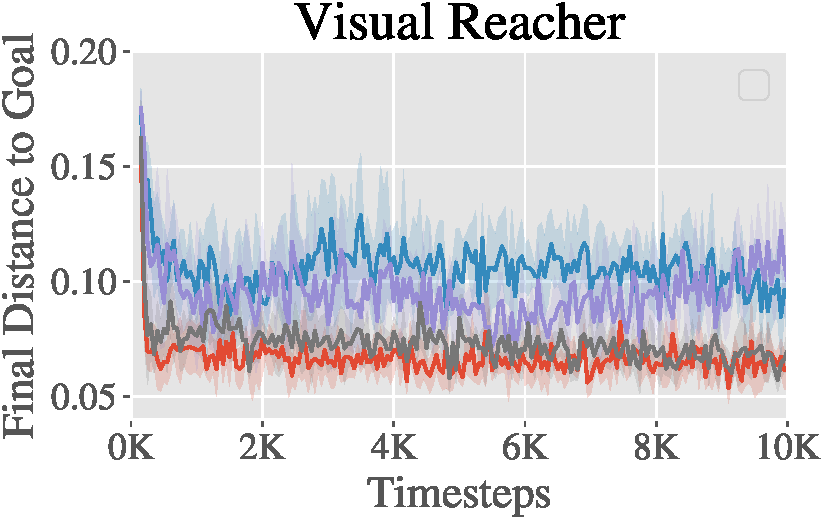
\includegraphics[height=0.185\linewidth]{img/reacher_relabeling_ablation.pdf}
    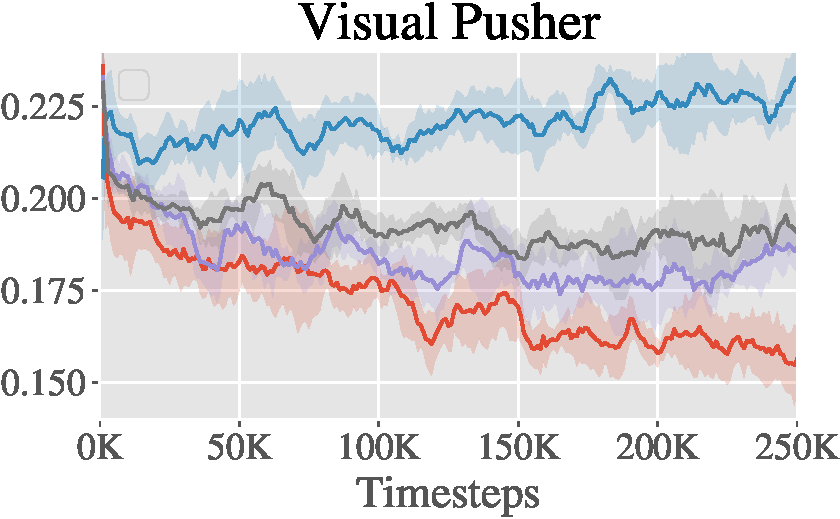
\includegraphics[height=0.185\linewidth]{img/pusher_relabeling_ablation.pdf}
    \includegraphics[height=0.185\linewidth]{img/multiobj_pusher_relabeling_ablation.pdf}
    \caption{Relabeling ablation simulated results, showing final distance to goal vs environment steps. RIG (red), which uses a mixture of VAE and future, consistently matches or outperforms the other methods.}
    \vspace{-0.1in}
    \label{fig:relabel-ablation-all-envs}
\end{figure}

\subsection{Reward type ablation}

In this experiment, we change only the reward function that we use to train the goal-conditioned valued function to show the effect of using the latent distance reward.
We include the following methods for comparison:
\textit{Latent Distance}, which is the reward used in RIG, i.e. $A = \mathbf{I}$ in Equation \eqref{eq:reward-log-prob-equivalence};
\textit{Log Probability}, which uses the Mahalanobis distance in Equation \eqref{eq:reward-log-prob-equivalence}, where $A$ is the precision matrix of the encoder;
and \textit{Pixel MSE}, which computes mean-squared error (MSE) between state and goal in pixel space. To compute the pixel MSE for a sampled latent goal, we decode the goal latent using the VAE decoder, $p_\psi$, to generate the corresponding goal image. Figure \ref{fig:reward-ablation-all-envs} shows the effect of different rewards with our method.

\begin{figure}[h]
    \centering
    % \includegraphics[height=0.25\linewidth]{img/reacher_reward_type_ablation_b.pdf}
    \includegraphics[height=0.19\linewidth]{img/reacher_reward_type_ablation.pdf}
    \includegraphics[height=0.19\linewidth]{img/pusher_reward_type_ablation.pdf}
    \includegraphics[height=0.19\linewidth]{img/multiobj_pusher_reward_type_ablation.pdf}
    \caption{Reward type ablation simulated results, showing final distance to goal vs environment steps. RIG (red), which uses latent distance for the reward, consistently matches or outperforms the other reward types.}
    \vspace{-0.1in}
    \label{fig:reward-ablation-all-envs}
\end{figure}

\subsection{Online training ablation} \label{sec:appendix_online}
Rather than pre-training the VAE on a set of images collected by a random policy, here we train the VAE in an online manner: the VAE is not trained when we initially collect data with our policy.
After every 3000 environment steps, we train the VAE on all of the images observed by the policy.
We show in Figure \ref{fig:online-ablation-all-envs} that this online training results in a good policy and is substantially better than leaving the VAE untrained.
These results show that the representation learning can be done simultaneously as the reinforcement learning portion of RIG, eliminating the need to have a predefined set of images to train the VAE.

The Visual Pusher experiment for this ablation is performed on a slightly easier version of the Visual Pusher used for the main results.
In particular, the goal space is reduced to be three quarters of its original size in the lateral dimension.

\begin{figure}[h]
    \centering
    \includegraphics[height=0.2\linewidth]{img/reacher_online_ablation.pdf}
    \includegraphics[height=0.2\linewidth]{img/pusher_online_ablation.pdf}
    \caption{Online vs offline VAE training ablation simulated results, showing final distance to goal vs environment steps. Given no pre-training phase, training the VAE online (red), outperforms no training of the VAE, and also performs well.}
    \vspace{-0.1in}
    \label{fig:online-ablation-all-envs}
\end{figure}

\subsection{Comparison to Hindsight Experience Replay} \label{sec:her_relabeling_ablation}

In this section, we study in isolation the effect of sampling goals from the goal space directly for Q-learning, as covered in Section~\ref{sec:goal-relabeling}.
Like hindsight experience replay \cite{andrychowicz2017her}, in this section we assume access to state information and the goal space, so we do not use a VAE.

To match the original work as closely as possible, this comparison was based off of the OpenAI baselines code \cite{plappert2018techreport} and we compare on the same Fetch robotics tasks. To minimize sample complexity and due to computational constraints, we use single threaded training with \texttt{rollout\_batch\_size=1, n\_cycles=1, batch\_size=256}. For testing, \texttt{n\_test\_rollouts=1} and the results are averaged over the last 100 test episodes. Number of updates per cycle corresponds to \texttt{n\_batches}.

On the plots, ``Future'' indicates
the future strategy as presented in \citet{andrychowicz2017her} with $k=4$. ``Ours'' indicates
resampling goals with probability 0.5 from the "future" strategy with $k=4$ and probability 0.5 uniformly from the environment goal space. Each method is shown with dense and sparse rewards.

\begin{figure}[H]
    \centering
    \includegraphics[height=0.2\linewidth]{img/her/push64.pdf}
    \includegraphics[height=0.2\linewidth]{img/her/slide64.pdf}
    \includegraphics[height=0.2\linewidth]{img/her/pick64.pdf} \\
    \includegraphics[height=0.2\linewidth]{img/her/push256.pdf}
    \includegraphics[height=0.2\linewidth]{img/her/slide256.pdf}
    \includegraphics[height=0.2\linewidth]{img/her/pick256.pdf}
    \caption{Comparison between our relabeling strategy and HER. Each column shows a different task from the OpenAI Fetch robotics suite. The top row uses 64 gradient updates per training cycle and the bottom row uses 256 updates per cycle. Our relabeling strategy is significantly better  for both sparse and dense rewards, and for higher number of updates per cycle.}
    \vspace{-0.1in}
    \label{fig:her64}
\end{figure}

Results are shown in Figure \ref{fig:her64}. Our resampling strategy with sparse rewards consistently performs the best on the three tasks. Furthermore, it performs reasonably well with dense rewards, unlike HER alone which often fails with dense rewards. While the evaluation metric used here, success rate, is favorable to the sparse reward setting, learning with dense rewards is usually more sample efficient on most tasks and being able to do off-policy goal relabeling with dense rewards is important for RIG.

Finally, as the number of gradient updates per training cycle is increased, the performance of our strategy improves while HER does not improve and sometimes performs worse. As we apply reinforcement learning to real-world tasks, being able to reduce the required number of samples on hardware is one of the key bottlenecks. Increasing the number of gradient updates costs more compute but reduces the number of samples required to learn the tasks.

\section{Hyperparameters}
Table \ref{table:hyperparams} lists the hyperparameters used for the experiments.
\begin{table}[h]
\centering
\begin{tabular}{c|c|c}
\hline
\textbf{Hyperparameter} & \textbf{Value} & \textbf{Comments}\\
\hline
Mixture coefficient $\lambda$ & $0.5$ & See relabeling strategy ablation \\
\# training batches per time step & $4$ & Marginal improvements after $4$\\
Exploration Policy & OU, $\theta = 0.15, \sigma = 0.3$ & Outperformed Gaussian and $\epsilon$-greedy\\
$\beta$ for $\beta$-VAE & $5$ & Values around $[1, 10]$ were effective \\
Critic Learning Rate &$10^{-3}$ & Did not tune\\
Critic Regularization & None & Did not tune\\
Actor Learning Rate & $10^{-3}$ & Did not tune\\
Actor Regularization & None & Did not tune\\
Optimizer & Adam & Did not tune\\
Target Update Rate $(\tau)$ & $10^{-2}$ & Did not tune\\
Target Update Period & $2$ time steps & Did not tune\\
Target Policy Noise & $0.2$ & Did not tune\\
Target Policy Noise Clip & $0.5$ & Did not tune\\
Batch Size & $128$ & Did not tune\\
Discount Factor & $0.99$ & Did not tune\\
Reward Scaling & $10^{-4}$ & Did not tune\\
Normalized Observations & False & Did not tune\\
Gradient Clipping & False & Did not tune\\
% Critic FC sizes & False & Did not tune\\
\hline
\end{tabular}
\vspace{0.1cm}
\caption{Hyper-parameters used for all experiments.}
\label{table:hyperparams}
\end{table}

\section{Environment Details}
Below we provide a more detailed description of the simulated environments.

\textit{Visual Reacher}: A MuJoCo environment with a 7-DoF Sawyer arm reaching goal positions.
The arm is shown on the left of Figure \ref{fig:sim_screenshot} with two extra objects for the Visual Multi-Object Pusher environment (see below).
The end-effector (EE) is constrained to a 2-dimensional rectangle parallel to a table. 
The action controls EE velocity within a maximum velocity. 
The underlying state is the EE position $e$, and the underlying goal is to reach a desired EE position, $g_e$. 

\textit{Visual Pusher}: A MuJoCo environment with a 7-DoF Sawyer arm and a small puck on a table that the arm must push to a target push.
Control is the same as in Visual Reacher.
The underlying state is the EE position, $e$ and puck position $p$.
The underlying goal is for the EE to reach a desired position $g_e$ and the puck to reach a desired position $p$. 

\textit{Visual Multi-Object Pusher}: A copy of the Visual Pusher environment with two pucks.
The underlying state is the EE position, $e$ and puck positions $p_1$ and $p_2$.
The underlying goal is for the EE to reach desired position $g_e$ and the pucks to reach desired positions $g_1$ and $g_2$ respectively also constrained to each half of the workspace.
Each puck and respective goal is initialized in half of the workspace.

Videos of our method in simulated and real-world environments can be found at \url{https://sites.google.com/site/visualrlwithimaginedgoals/}.
\chapter{Appendix: Learning to Adapt in Dynamic, Real-World Environments through Meta-Reinforcement Learning
}
\noindent\makebox[\linewidth]{\rule{\linewidth}{3.0pt}}
\begin{center}
\LARGE{\textbf{Supplementary Material}}
\end{center}
\noindent\makebox[\linewidth]{\rule{\linewidth}{0.8pt}}

\section{Complete Ablative Results} \label{sec:appendix}

\subsection{Relabeling strategy ablation} \label{sec:appendix_relabeling_ablation}

In this experiment, we compare different goal resampling strategies for training the Q function. We consider:
\textit{Future},
relabeling the goal for a transition by sampling uniformly from future states in the trajectory as done in \citet{andrychowicz2017her};
\textit{VAE}, sampling goals from the VAE only;
\textit{RIG}, relabeling goals with probability $0.5$ from the VAE and probability $0.5$ using the future strategy;
and \textit{None}, no relabeling. 
Figure \ref{fig:relabel-ablation-all-envs} shows the effect of different relabeling strategies with our method.

\begin{figure}[h]
    \centering
    \includegraphics[height=0.185\linewidth]{img/reacher_relabeling_ablation.pdf}
    \includegraphics[height=0.185\linewidth]{img/pusher_relabeling_ablation.pdf}
    \includegraphics[height=0.185\linewidth]{img/multiobj_pusher_relabeling_ablation.pdf}
    \caption{Relabeling ablation simulated results, showing final distance to goal vs environment steps. RIG (red), which uses a mixture of VAE and future, consistently matches or outperforms the other methods.}
    \vspace{-0.1in}
    \label{fig:relabel-ablation-all-envs}
\end{figure}

\subsection{Reward type ablation}

In this experiment, we change only the reward function that we use to train the goal-conditioned valued function to show the effect of using the latent distance reward.
We include the following methods for comparison:
\textit{Latent Distance}, which is the reward used in RIG, i.e. $A = \mathbf{I}$ in Equation \eqref{eq:reward-log-prob-equivalence};
\textit{Log Probability}, which uses the Mahalanobis distance in Equation \eqref{eq:reward-log-prob-equivalence}, where $A$ is the precision matrix of the encoder;
and \textit{Pixel MSE}, which computes mean-squared error (MSE) between state and goal in pixel space. To compute the pixel MSE for a sampled latent goal, we decode the goal latent using the VAE decoder, $p_\psi$, to generate the corresponding goal image. Figure \ref{fig:reward-ablation-all-envs} shows the effect of different rewards with our method.

\begin{figure}[h]
    \centering
    % \includegraphics[height=0.25\linewidth]{img/reacher_reward_type_ablation_b.pdf}
    \includegraphics[height=0.19\linewidth]{img/reacher_reward_type_ablation.pdf}
    \includegraphics[height=0.19\linewidth]{img/pusher_reward_type_ablation.pdf}
    \includegraphics[height=0.19\linewidth]{img/multiobj_pusher_reward_type_ablation.pdf}
    \caption{Reward type ablation simulated results, showing final distance to goal vs environment steps. RIG (red), which uses latent distance for the reward, consistently matches or outperforms the other reward types.}
    \vspace{-0.1in}
    \label{fig:reward-ablation-all-envs}
\end{figure}

\subsection{Online training ablation} \label{sec:appendix_online}
Rather than pre-training the VAE on a set of images collected by a random policy, here we train the VAE in an online manner: the VAE is not trained when we initially collect data with our policy.
After every 3000 environment steps, we train the VAE on all of the images observed by the policy.
We show in Figure \ref{fig:online-ablation-all-envs} that this online training results in a good policy and is substantially better than leaving the VAE untrained.
These results show that the representation learning can be done simultaneously as the reinforcement learning portion of RIG, eliminating the need to have a predefined set of images to train the VAE.

The Visual Pusher experiment for this ablation is performed on a slightly easier version of the Visual Pusher used for the main results.
In particular, the goal space is reduced to be three quarters of its original size in the lateral dimension.

\begin{figure}[h]
    \centering
    \includegraphics[height=0.2\linewidth]{img/reacher_online_ablation.pdf}
    \includegraphics[height=0.2\linewidth]{img/pusher_online_ablation.pdf}
    \caption{Online vs offline VAE training ablation simulated results, showing final distance to goal vs environment steps. Given no pre-training phase, training the VAE online (red), outperforms no training of the VAE, and also performs well.}
    \vspace{-0.1in}
    \label{fig:online-ablation-all-envs}
\end{figure}

\subsection{Comparison to Hindsight Experience Replay} \label{sec:her_relabeling_ablation}

In this section, we study in isolation the effect of sampling goals from the goal space directly for Q-learning, as covered in Section~\ref{sec:goal-relabeling}.
Like hindsight experience replay \cite{andrychowicz2017her}, in this section we assume access to state information and the goal space, so we do not use a VAE.

To match the original work as closely as possible, this comparison was based off of the OpenAI baselines code \cite{plappert2018techreport} and we compare on the same Fetch robotics tasks. To minimize sample complexity and due to computational constraints, we use single threaded training with \texttt{rollout\_batch\_size=1, n\_cycles=1, batch\_size=256}. For testing, \texttt{n\_test\_rollouts=1} and the results are averaged over the last 100 test episodes. Number of updates per cycle corresponds to \texttt{n\_batches}.

On the plots, ``Future'' indicates
the future strategy as presented in \citet{andrychowicz2017her} with $k=4$. ``Ours'' indicates
resampling goals with probability 0.5 from the "future" strategy with $k=4$ and probability 0.5 uniformly from the environment goal space. Each method is shown with dense and sparse rewards.

\begin{figure}[H]
    \centering
    \includegraphics[height=0.2\linewidth]{img/her/push64.pdf}
    \includegraphics[height=0.2\linewidth]{img/her/slide64.pdf}
    \includegraphics[height=0.2\linewidth]{img/her/pick64.pdf} \\
    \includegraphics[height=0.2\linewidth]{img/her/push256.pdf}
    \includegraphics[height=0.2\linewidth]{img/her/slide256.pdf}
    \includegraphics[height=0.2\linewidth]{img/her/pick256.pdf}
    \caption{Comparison between our relabeling strategy and HER. Each column shows a different task from the OpenAI Fetch robotics suite. The top row uses 64 gradient updates per training cycle and the bottom row uses 256 updates per cycle. Our relabeling strategy is significantly better  for both sparse and dense rewards, and for higher number of updates per cycle.}
    \vspace{-0.1in}
    \label{fig:her64}
\end{figure}

Results are shown in Figure \ref{fig:her64}. Our resampling strategy with sparse rewards consistently performs the best on the three tasks. Furthermore, it performs reasonably well with dense rewards, unlike HER alone which often fails with dense rewards. While the evaluation metric used here, success rate, is favorable to the sparse reward setting, learning with dense rewards is usually more sample efficient on most tasks and being able to do off-policy goal relabeling with dense rewards is important for RIG.

Finally, as the number of gradient updates per training cycle is increased, the performance of our strategy improves while HER does not improve and sometimes performs worse. As we apply reinforcement learning to real-world tasks, being able to reduce the required number of samples on hardware is one of the key bottlenecks. Increasing the number of gradient updates costs more compute but reduces the number of samples required to learn the tasks.

\section{Hyperparameters}
Table \ref{table:hyperparams} lists the hyperparameters used for the experiments.
\begin{table}[h]
\centering
\begin{tabular}{c|c|c}
\hline
\textbf{Hyperparameter} & \textbf{Value} & \textbf{Comments}\\
\hline
Mixture coefficient $\lambda$ & $0.5$ & See relabeling strategy ablation \\
\# training batches per time step & $4$ & Marginal improvements after $4$\\
Exploration Policy & OU, $\theta = 0.15, \sigma = 0.3$ & Outperformed Gaussian and $\epsilon$-greedy\\
$\beta$ for $\beta$-VAE & $5$ & Values around $[1, 10]$ were effective \\
Critic Learning Rate &$10^{-3}$ & Did not tune\\
Critic Regularization & None & Did not tune\\
Actor Learning Rate & $10^{-3}$ & Did not tune\\
Actor Regularization & None & Did not tune\\
Optimizer & Adam & Did not tune\\
Target Update Rate $(\tau)$ & $10^{-2}$ & Did not tune\\
Target Update Period & $2$ time steps & Did not tune\\
Target Policy Noise & $0.2$ & Did not tune\\
Target Policy Noise Clip & $0.5$ & Did not tune\\
Batch Size & $128$ & Did not tune\\
Discount Factor & $0.99$ & Did not tune\\
Reward Scaling & $10^{-4}$ & Did not tune\\
Normalized Observations & False & Did not tune\\
Gradient Clipping & False & Did not tune\\
% Critic FC sizes & False & Did not tune\\
\hline
\end{tabular}
\vspace{0.1cm}
\caption{Hyper-parameters used for all experiments.}
\label{table:hyperparams}
\end{table}

\section{Environment Details}
Below we provide a more detailed description of the simulated environments.

\textit{Visual Reacher}: A MuJoCo environment with a 7-DoF Sawyer arm reaching goal positions.
The arm is shown on the left of Figure \ref{fig:sim_screenshot} with two extra objects for the Visual Multi-Object Pusher environment (see below).
The end-effector (EE) is constrained to a 2-dimensional rectangle parallel to a table. 
The action controls EE velocity within a maximum velocity. 
The underlying state is the EE position $e$, and the underlying goal is to reach a desired EE position, $g_e$. 

\textit{Visual Pusher}: A MuJoCo environment with a 7-DoF Sawyer arm and a small puck on a table that the arm must push to a target push.
Control is the same as in Visual Reacher.
The underlying state is the EE position, $e$ and puck position $p$.
The underlying goal is for the EE to reach a desired position $g_e$ and the puck to reach a desired position $p$. 

\textit{Visual Multi-Object Pusher}: A copy of the Visual Pusher environment with two pucks.
The underlying state is the EE position, $e$ and puck positions $p_1$ and $p_2$.
The underlying goal is for the EE to reach desired position $g_e$ and the pucks to reach desired positions $g_1$ and $g_2$ respectively also constrained to each half of the workspace.
Each puck and respective goal is initialized in half of the workspace.

Videos of our method in simulated and real-world environments can be found at \url{https://sites.google.com/site/visualrlwithimaginedgoals/}.

\end{document}
